\documentclass[11pt]{usuthesis}
\usepackage{graphicx}
%\usepackage[draft]{graphicx}

\usepackage{alltt,makeidx,ifthen,fancyvrb,listings}
\usepackage{hyperref,overpic,lscape}
\usepackage[below]{placeins}
\usepackage{subfigure,color}
\usepackage{layout,afterpage,longtable}
\usepackage{amsfonts,eucal,amssymb}
\usepackage{amsmath}
\usepackage{flafter}
\usepackage{url}
\usepackage{afterpage} % to clear floating objects
%\usepackage{algorithm}
\usepackage{algorithm2e}
% use ImageMagrick
%\DeclareGraphicsRule{.jpg}{eps}{.bb}{`convert #1 eps:-}%
\renewcommand{\baselinestretch}{1}
\urlstyle{rm}

\makeatletter
%%%%%%%%%%%%%%%%%%%%%%%%%%%%%% User specified LaTeX commands.
% \newcounter{problem}
% \newcommand{\prob}{ \addtocounter{problem}{1}  {\bf Problem \arabic{problem}}:\  }
\newcommand{\uc}{~Uci\'{n}ski}
\newcommand{\dt}{\hbox{d}t}
\newcommand{\fwA}{\textwidth} % one column
\newcommand{\fwB}{0.8\textwidth} % one column
\newcommand{\fwC}{0.5\textwidth}


%%%%%%%%%%%%%%%% zsong's macros
\newtheorem{thm}{Theorem}[section]
\newtheorem{cor}[thm]{Corollary}
\newtheorem{lem}[thm]{Lemma}
\newtheorem{mdef}[thm]{Definition}
\newenvironment{proof}[1][Proof]{\begin{trivlist}
\item[\hskip \labelsep {\bfseries #1}]}{\end{trivlist}}
\newcommand{\qed}{\nobreak \ifvmode \relax \else
      \ifdim\lastskip<1.5em \hskip-\lastskip
      \hskip1.5em plus0em minus0.5em \fi \nobreak
      \vrule height0.75em width0.5em depth0.25em\fi}

\newenvironment{definition}[1][Definition]{\begin{trivlist}
\item[\hskip \labelsep {\bfseries #1}]}{\end{trivlist}}
\newenvironment{example}[1][Example]{\begin{trivlist}
\item[\hskip \labelsep {\bfseries #1}]}{\end{trivlist}}
\newenvironment{remark}[1][Remark]{\begin{trivlist}
\item[\hskip \labelsep {\bfseries #1}]}{\end{trivlist}}

%% for floating object
%\renewcommand{\topfraction}{.85}
%\renewcommand{\bottomfraction}{.7}
%\renewcommand{\textfraction}{.35}
\renewcommand{\floatpagefraction}{.7}

%\renewcommand{\topfraction}{.85}
%\renewcommand{\bottomfraction}{.7}
%\renewcommand{\textfraction}{.15}
%\renewcommand{\floatpagefraction}{.66}
%\renewcommand{\dbltopfraction}{.66}
%\renewcommand{\dblfloatpagefraction}{.66}
%\setcounter{topnumber}{9}
%\setcounter{bottomnumber}{9}
%\setcounter{totalnumber}{20}
%\setcounter{dbltopnumber}{9}

%%%%%%%%%%%%%%%% end of zsong's macros


\makeatother

\author{Zhen Song}
\title{Observation Problems Involving Wireless Sensor Networks (draft 7)}

\departmentname{Electrical and Computer Engineering}
\degreein{Electrical Engineering}
\firstreader{Dr. Brandon Eames}
\secondreader{Dr. Jake Gunther}
\thirdreader{Dr. Wei Ren}
\forthreader{Dr. Vlademir Kulyukin}
\graddean{Dr. Thomas Kent}
\deantitle{Dean of Graduate Studies}
\majorprof{Dr. YangQuan Chen}
\dissertation{Dissertation}
\degree{Doctor of Philosophy}
\degreenotallcaps{Doctor of Philosophy}
\date{\today}
\year{2007}
\makeindex



\begin{document}
\maketitle
\begin{dedication}
  To my family, for their encouragements and supports. 
\end{dedication}


\begin{abstract}
An important application of wireless sensor networks is to observe the physical world. This dissertation focuses on observation methods by wireless sensor networks (WSNs), especially the unique issues due to the properties of WSNs.

    Mobility is an important feature of WSNs. Since the quality of the observation on the physical world depends on the positions of the sensors, the optimum sensor positions depend on the models of the physical systems. Mobile sensor networks can provide better estimates, since the sensor nodes can maneuver to the optimal sensing positions.
       In Chapter~\ref{s:MasnetIROS}, we study a problem called trajectory optimization for observation on Distributed Parameter Systems (DPSs). Given a model of a distributed parameter system, we proposed a numeric method to compute the optimal trajectory of mobile sensors, which are mounted on differentially-driven robots, such that the observation on the system parameter is optimized.

    Energy efficiency is the key challenge and the central research topic for WSNs. For WSN-based observation system, it is important to balance the tradeoff between the energy efficiency and estimation precision. Energy costs can be reduced significantly by selecting proper sensors. In Chapter~\ref{s:COSS}, we propose a convex optimal sensor selection (COSS) algorithm to choose proper sensors to observe parameters of physical systems, such as the position of a target. After introducing several approximations, we formulate the sensor selection problem as a convex optimization problem. Unlike common optimization formulations, we do not explicitly minimize the number of selected sensors. Our cost function is constructed to minimize estimation errors. However, due to the properties of the convex optimization, the number of selected sensors is minimized simultaneously during the time when the estimation error is minimized, which is referred as the implicit optimal sensor selection (IOSS). Our analysis provides some guidance on how to design and tune the IOSS methods. We prove that those IOSS methods not only select the minimum number of sensors that allowed by the Carath\'{e}odory's theorem, but also approximate the minimal estimation error predicted by the Cram\'{e}r-Rao lower bound (CRLB). In addition, we have tested the COSS algorithm by extensive simulation and hardware experiments. Those experiments are conducted under realistic conditions that are close to the real-world engineering practices.

    Localization is a fundamental problem for WSNs.
    The sensors' positions are required by most of the high-level WSN applications. In Chapter~\ref{s:loc}, an asynchronous TDOA localization method is proposed. When there are a large number of sensor nodes whose positions are unknown, asynchronous TDOA methods reduce communication costs as well as the beacon nodes' hardware costs. The positioning error of the localization system is affected by the placement of the beacon notes. In order to guarantee the robustness of the localization system, the beacon placement problem is formulated as a min-max optimization. The optimization is solved by semi-infinite programming method.

    Although the above problems are not identical, they share the same theoretical framework, i.e, optimal experimental design. They are formulated as convex optimization on cost functions based on the Fisher information matrix (FIM). FIM and convex analysis are promising mathematical tools for WSN-based signal processing.
    % The properties of convex optimization play important roles during the procedure to solve those practical problems.
\end{abstract}




\begin{acknowledgements}
    This dissertation is a summary of my research in Utah State University and Siemens Corporate Research. In Utah State University, my research was under the guidance of my PhD advisor, Dr.~YangQuan Chan, and my Master advisor, Dr.~Kevin Moore. During my internship in Siemens Corporate Research, Dr.~Chellury Ram Sastry gave me many insightful advices. They always encourage me to focus on the fundamental problems and continuously improve my ideas by critical thinking. This is the best education experiences I have ever had in my life. I sincerely appreciate their time and efforts on helping me, including the PhD advices as well as the training on my mind.

    I feel really lucky since there are so many people who helped me on my research. Dr.~Dariusz Uci\'{n}ski, Dr.~Ren Wei, Dr.~Vladimeir Kulyukin and Dr.~Jacob Gunther gave me lots of valuable advices. The discussions with them really helped my research. Hereby I also appreciate my other committee members and past committee members, Dr.~Brandon Eames, Dr.~Matthew Berkemeier, and Dr.~Nick Flann.

    I want to sincerely thank all the people who had ever helped the MAS-net project, including the advisors, Dr.~Kevin Moore and Dr.~YangQuan Chen; the team members, PengYu Chen, ZhongMin Wang, Anisha Arora, HaiYang Chao and William Burgeous; the CSOIS members, Dr.~Lili Ma, Dr.~JinSong Liang, Dan Storment; Especially, I want to thank PengYu Chen for his significant contributions to the MAS-net project. Without him, the achievement is not possible.

    In the past several years, I have learned much from the discussions or collaborations with my colleagues. Hereby I present my appreciation to them. Nazif Cihan Tas, XiaoChun Xu, Vehbi Cagri Gungor. I am grateful for the various of help from my friends, Dr.~Hyo-Sung Ahn, Dr.~Dong Wei, Peng Zhao, Tian Xia, Michael Frashinger, Stanislava Soro.

\vspace{.2in}
\hfill Zhen Song
\end{acknowledgements}





\tableofcontents
\listoftables
\listoffigures
\body



\chapter{Introduction}\label{s:intro}
\section{Background And Literature Review}
\subsection{What is Sensor Network}
Sensor network~\cite{AkyildizSurveySN} is considered as ``one of the important technologies of the 21st century''~\cite{ChongSensornet}. In general, sensor network is referring to sensors that has been connected by computer networks. The sensors measure physical quantities of the world, while computer networks integrate and interpret sensor data.

This concept was proposed decades ago. For example, it is common to see networked data acquisition (DAQ) systems, such as Labview systems\cite{labview}, in industry. However, many researchers have recognized that the modern computer, sensor and communication technologies has significantly changed the sensor networks.

Since microprocessors are very affordable now, sensor data can be processed by local processors before being transmitted to the base station, or the sink. The concept of ``smart sensor'' can be realized recently.

% \item MEMS technologies significantly reduce the size and cost of many sensors. For example, it is easy to buy a finger-nail size MEMS accelerometer chip under \$20 today. It can powered by batteries. In the past, accelerometers are in the size of tens of centimeters and can hardly to powered by batteries.

Communication technologies, either wired or wireless, are significantly improved in the past several years. Wireless technologies are especially under fast developments. %For example, the sizes, price and power consumptions of modern cell phones are significantly reduced in the past several years.
More and more new communication technologies have been developed. WiFi, Bluetooth, CDMA, UWB, etc. Comparing to the past, it is much easier to connect thousands of sensor nodes with the help of those new technologies.


     Due to these new enabling technologies, the methods to deploy sensors and collect the sensor data are also different from before. In general, those new technologies have potentials to reduce the cost of sensor networks, improve the energy efficiency, network scalability and reliability. How to properly use those new technologies is an active research topic.

The sensor networks can be classified into different categories. Among them, wireless sensor network (WSN)~\cite{ZhaoGuibasWSN2004,akyldizSurvey} and distributed sensor network (DSN)~\cite{Qi01survey} are among the two most important categories of sensor networks. This dissertation focuses on WSNs.


\subsection{Introduction to WSN}
WSNs~\cite{ZhaoGuibasWSN2004,akyldizSurvey,Estrin01Instrumenting} are not just traditional sensor networks with wireless communications. In fact, the philosophy of WSNs is different from other sensor networks in the past. The deployment methods, power consumption requirements and network protocols for WSNs are different than those wired sensor networks.

    Currently, the computer and communication technologies have arrived in a stage where the hardware cost is so low that massive dense deployment of the wireless sensor nodes is affordable. A densely deployed WSN provides more samples on the physical world and improves the observation. However, the costs of replacing batteries for large scale sensor networks are significant.
    It is very important to improve the network life time by various of energy saving methods.
      The energy efficient protocols of WSN are under active research. Comparing to generic wireless communication protocols, the energy efficient protocols of WSN commonly uses knowledge on the structure of the sensor data to improve the performance. For example, data-centric routing approach~\cite{Krishnamachari_infocom02} is proposed to replace IP-based routing: the route is computed based on the relative position between the data and the sensors, instead of IP addresses of the sensors. In addition, due to the nature of wireless communication, the topology of the network is not statics. The wireless communication protocols must adjust the route accordingly~\cite{rangwala06}.

    The future of WSN may come to the scenario of ``smart dust''\cite{PisterSmartdust01}: each sensor node is very small, even close to the size of dust. On the sensor nodes, microprocessors, sensors, communication devices, or energy harvesting apparatus are fully integrated. To explore the capability of the sensors, the sensor nodes are deployed in massive scales at high densities. Comparing to traditional sensor networks, the WSNs are in larger scale and normally work in distributed fashion.


The following items are some common features of wireless sensor networks:

\begin{itemize}
\item The WSN protocols support large scale networks.
For example, IEEE 802.15.4 standard~\cite{Standard802.15.4.2003} is used in some sensor network products. The standard supports $2^{32}$ sensor nodes per network, in theory.
    In the literature of sensor network protocol design, it is common to see that a certain algorithm is tested on a network with tens of sensor nodes~\cite{rangwala06,WelshMoteTrack_LoCA2005-PUC} and simulated with hundreds or thousands of nodes~\cite{VuranSpatioTemporal04,Qi01survey}.
 The sizes of WSNs are in larger scales comparing to most of other wireless communication protocols. For example, the Bluetooth standard was designed for Wireless Personal Area Network (WPAN) in stead of sensor network. The Bluetooth standard only supports 8 devices per network~\cite{wiki:piconet}.
\item The costs of wireless communication are relatively low, in terms of money, energy and computation. For example, the maximum power consumption of Telos mote, an example of WSN sensor node, is in the level of tens milliwatts and the communication stack is small enough for low cost microprocessors~\cite{Polastre-telos}. The price of that Telos sensor node is around \$70 at the moment. As a comparison, WiFi (IEEE 802.11) devices are normally powered by wires, instead of by common AA batteries, because their energy consumption is much higher. In addition, WiFi devices are normally more costly and have larger form factors.
\item The sensor nodes have certain computing capabilities. Sensor data are normally pre-processed on the sensor nodes. The pre-processing could be data filtering, compression, or encryption on the information of interest. For example, the sensor data may be stored on a local database~\cite{GehrkeQueryProc2004} and the node only delivers the data that are queried by the base station. Taking the advantages of the on-board processing power the valuable communication resources are used for efficiently.
\item The sensor nodes are normally deployed densely. Usually, dense deployment is more preferable as far as it is affordable. A denser deployment provides better estimation resolution on the physical world.
\item Sensor networks are normally supported by specially designed communication hardware or protocols. Due to the difference between sensor data and generic communicate data, such as speech or video, the generic communication systems are not the most efficient approach for sensor data transportation. For example, instead of pursuing high communication speed, as many other communication standards do, the IEEE 802.15.4 standard employs low rate communication. Since high speed is not required by many sensor systems, adopting low rate communication is a better strategy, in terms of cost, size and energy requirements, etc.
\end{itemize}

    %The difference between WSNs and traditional sensor networks are listed in the followings:
%
%\begin{itemize}
%\item Energy efficiency is of vital importance to WSNs. Given the large number of sensors, it is often very hard to replace the batteries on each of the sensor nodes. Although different hardware have been constructed to harvest energy in the environments, the available energy is still very limited. Thus, energy efficiency is the essential consideration for WSN hardware and software designs, communication protocols and information processing algorithms. Many existing algorithms, such as the standard target tracking problems, are developed for generic sensor network, and thus they do not consider energy efficiency.
%\item WSNs are distributed systems: not only the data are distributed among different sensors, the computation are usually distributed too.
%% It is desirable to execute on those
%     Unlike the traditional sensors, each sensor node of a WSN has computation capability. Thus, sensor data are normally filtered before being transmitted to the base station. Since the energy cost for the filtering is much less than the energy used for wireless transmission, computation on the sensor could significantly reduce the total energy cost.
%
%% \item The existing networking protocols, such as TCP/IP, Fieldbus, etc., do not satisfy the requirements of WSNs. A fundamental reason is that WSNs are normally data centric.
%\end{itemize}




WSN can be used in a wide variety of remote monitoring and control applications ranged from environmental and human body monitoring~\cite{MalanCodeBlue}
 to military surveillance~\cite{OgrenCooperativeControl, dutta06radar, DutteLitespaper}, building automation~\cite{Crossbow2006}, industrial monitoring and control~\cite{KevanShipboardPM06}, homeland security~\cite{SimonCountersniper2004}, air pollution detection~\cite{LiuDualSpaceAppTracking}, wild fire monitoring~\cite{DoolinaFirebugSPIE05}, detection of persons and
vehicles in open areas~\cite{DuttamirMote}, and reconnaissance tasks~\cite{ZhaoGuibasWSN2004}, etc..
    In typical remote monitoring applications, sensor nodes are deployed in an ad hoc manner over an area of interest.
Individual sensor nodes can measure physical quantities and communicate sensing information to other sensors or to a sink (base station) by radio. Furthermore, sensor nodes have a limited ability to process information on an on-board CPU, and can store that information in memory. This is the reason why such wireless sensors are sometimes referred to as smart sensors or smart dust. The
on-sensor processing and on-sink processing should cooperatively interpret sensor data to observe environments in energy efficient approaches. Although each individual node has limited capability, several such nodes can cooperate to accomplish complex tasks. To put it succinctly, WSNs provide the ability to connect the physical world to enterprize computing systems, thereby improving business processes and facilitating efficient decision making.



\subsection{Research on WSNs from Different Aspects}
As an interdisciplinary topic, WSNs have been studied from many different aspects by researchers from different backgrounds. Because the interpretation on the sensor data and the structure of the sensor data are application-dependent, to our best knowledge, there is no unified theory that integrates all the sensor network design problems into one framework. Most of the research in sensor network are conducted under the guidance of one of the following aspects:
\begin{itemize}
  \item Communication and networking aspect: how to send information by WSNs.
  \item Signal and system aspect: what information are useful and should be sent.
  \item Data and service aspect: how to store and query data.
\end{itemize}

Hereby we classify and review the current literatures based on the proposed classification methods.

\subsubsection{Communication and networking}
WSNs can be considered as networked communication systems. From the aspect of networking, new protocols or communication devices can be designed, in order to transport the input data to the sink and satisfies certain quality of services (QoS). Some examples of commonly considered QoS include network throughput, packet reception rate, delay, etc.

    In the comprehensive survey for the protocols of sensor networks~\cite{AkyildizSurveySN}, the differences between WSNs and traditional ad hoc networks are summarized as the follows:
\begin{itemize}
  \item WSNs are deployed in much larger numbers with higher densities, and prone to failures.
  \item The topologies of WSNs are frequently changing.
  \item Sensor nodes have limited capabilities of power, computation and memory.
  \item Each sensor node may not have an unique ID.
\end{itemize}


WSNs are also compared with the Internet~\cite{CullerOverviewWSN05,Estrin01Instrumenting}.
\begin{itemize}
  \item Self-organizing is more important for WSNs.
  \item The routing method used in the Internet is not practical for WSNs. Instead, routing methods based on sensor location or sensor values may be more effective.
  \item Constraints on bandwidth and energy are more limited for WSNs.
\end{itemize}


    Traditionally, computer networks are implement by different layers. The classical TCP/IP model has 5 layers. They are physical layer, data link layer, network layer, transport layer, and application layer. Most of the layers have their counterparts in WSN protocols.


    On the physical layer, the central task is to develop low-cost and energy-efficient radios, on which both the academia and industry are keep proposing new solutions~\cite{korber05embedding,Standard802.15.4.2003,SensicastEMS,White_Paper_nanoNET-2,Rabaey2000b}. On the data link layer, different Media Access Control (MAC) protocols are proposed. Some are developed for general sensor networks~\cite{YeSmac_infocom02} and some are designed  for specific application~\cite{VuranSpatioTemporal04}.
    The network layer is responsible for network routing. Common routing metrics include the number of hops, RSSI, and link quality, etc.~\cite{Multihop2003}. %The structure of the sensor data are also used for routing~\cite{EstrinDirectedDiff}.

    This layered network communication model is widely adopted. However, since it was developed for generic communication, it may not satisfy the requirements of WSNs. As paper~\cite{CullerPlostreSNA} observed, a key challenge of the current sensor network systems is the lack of a general communication model. Many protocols behave well with them alone, but does not cooperate with each other. In fact, the layered model is not the only solution. For example, hybrid designs do not follow the layered model~\cite{CullerPlostreSNA,AkyildizSurveySN}. In the hybrid models, one or several modules are operating cross several layers.

    In summary, WSNs can be considered as a new type of computer networks. In addition to pursuit classical network performances, such as high throughput, high packet reception rate (PRR), and low message delivery delay, some new criteria, such as energy efficiency, fault tolerance and scalability, should also be considered.
        A good network model should be able to balance different performances and trade off the costs, in order to satisfy individual applications as much as possible.


    % In our opinion, the difficulty mainly come from the fact that sensor networks are not just communication systems. They are frequently also observers of complex systems. Thus, although the layered model was very successful in the Internet, the model may not be suitable for the whole sensor network.

\subsubsection{Signal and system}
WSNs are commonly used to observe physical systems. The sensor measurements can be considered as signals, while the network is an imperfect communication channel, which introduces delays and packet drops, etc. Thus, there are many challenges on signal processing and system identifications for WSNs. The follows are some examples.
\begin{itemize}
  \item Sensor calibration: Unlike the calibration for a single-sensor system, calibration on sensor networks is more complex. Since there are normally a large number of sensors in the network, it is normally impossible to manually calibrate sensors one by one. Automatic and systematic calibration methods are required~\cite{FengActSenCal2006,WhitehouseCuller2005}.
  \item Sensor selection and placement: Due to the properties of the physical systems, the ``quality'' of the sensor data is position-dependent. In order to save the communication energy, we need to ensure that just enough ``good'' data are sent through the communication channels; no ``bad'' data or ``more than enough'' data should be transmitted.
  %only high quality data should be transmitted and used for system estimations.
   It is important to select sensors or positions of the sensors based on the quality of their sensing data~\cite{zhao03collaborative,WangEstrinInfomationSS05,VuranSpatioTemporal04,YickOptBeaconPlacement04}.
  \item Mobility of sensor node: Mobile sensor nodes are feasible in the context of WSNs. Some methods are proposed to take the advantages of the mobility of sensor nodes for better sensing~\cite{SongOptMobileSensIROS05,CaoDiffGame2006,Meliou2006,MurrayDecActiveSensing}.
  \item Detection and estimation: It is desirable to have distributed detection or estimation algorithms, in order to enhance the scalability and fault tolerance of WSNs. For example, distributed regression~\cite{Guestrin2004}, distributed least squares fitting~\cite{XiaoBoydLallp2p_ls} and other distributed algorithms~\cite{RossiMonitoringDif,LiuDualSpaceAppTracking} are discussed.
  \item Target tracking: As an extension to the classic target tracking problem, energy efficient or distributed tracking are discussed~\cite{SAM2006Amit,FZhaoShinInfoDrivenDynamicTracking,AslamBinaryTrackingWSN2003,ArandaOptSensorPlacement05},
   under the context of WSNs.
\end{itemize}


Of course, there are much overlapping on the above topics. For example, Aranda et al take the advantages of the mobility of robotic wireless sensor nodes to track targets~\cite{ArandaOptSensorPlacement05}.

% The intuition is easy to understand. However, in practice, it may not be trivial to judge the quality of a sensor data, or decide when ``enough'' data have been collected. For instances, the examples in papers~\cite{isler06tase,VuranSpatioTemporal04} indicate that a small number of sensors may provide estimation as good as many sensors.
%    The theories on information, signal processing, control system and statistics provide tools to quantify the quality and quantity of the information.


%The theory on signal processing shows us the intrinsic properties of the incoming signals, i.e., the sensor data. For example, the uncertainty of information can be quantified by entropy. The higher the uncertainty, the bigger the entropy.
%
%In~\cite{wang04entropybased}

The knowledge on the physical model of the system under observation may significantly improve estimation precision and reduce the energy cost.
    For example, we may want to deploy a WSN-based predictive maintenance system on an expensive engine~\cite{KevanShipboardPM06} to predict possible failures in future. If the model of the engine is known, some important questions can be answered. By analyzing the physical model of the engine, we can determine the observability of an internal physical quantity, e.g., an internal state. If it is not observable, then the quantity can not be estimated, no matter how many sensors are installed.
        Based on the model, the sensor deployment can be optimized.         For example, one approach for the optimal sensor placement problem is to formulate it as a convex optimization problem.
        The problem can be solved under the framework of optimal experiment design~\cite{UcinskiOptDPS05,fedorov94optimal,MurrayDecActiveSensing}.



\subsubsection{Data and service}
Wireless sensor networks can be considered as distributed database systems. The users may query the data that have been collected by the sensor nodes. Due to the unique properties of the WSNs, the queries on WSNs are not the same as the queries on standard databases.

For WSNs, the users are interested in high level information, and data aggregations are usually required. For example, one may query ``the averaged temperature of the 4th floor,'' instead of the measurements on temperature values of each sensor. One method to implement the above query is to aggregate the sensor data at sink~\cite{GehrkeQueryProc2004}.


Although the query on WSN can be considered as a special routing problem~\cite{madden02design} and implemented by the standard address-centric routing, this approach may not be efficient, since the raw sensor data have much redundant information. It may be more efficient to transmit raw data by the address-centric routing methods, where the sensor data may be aggregated during the transmission. The route may be affected by the sensor data~\cite{Krishnamachari_infocom02}.



\section{Dissertation Motivation and Application Scenarios}
\subsection{Motivation and Scenarios of MAS-net}
        Chapter~\ref{s:MasnetIROS} is motivated by our project named MAS-net, which stands for mobile actuator-sensor networks (MAS-net)~\cite{MooreChen04,MASnetSPIE04ZoneControl,masnetspie04pathplan, ZhongminRobio04, PchenMS, AnishaMS}.
    This project is proposed to combine the latest sensor network technologies with robotics technologies for an application-oriented high-level tasks, namely, characterize, estimate and control diffusion process by networked mobile actuators and sensors.


The future working scenario of the MAS-net system is presented in~\cite{Moorewhitepaper03,MooreChen04}. Hereby we review it in brief. The scenario is shown in Fig.~\ref{f:app}. The numbers of the following comments are associated with the plots with the same numbers in Fig.~\ref{f:app}.
\begin{enumerate}
\item In the middle of a city, terrorists release a plume of chemical, biological, radiological (CBR) fog to the air. The diffusion of the plume is influenced by the
city building structures and the air flow. The poisonous plume is detected by a static sensor network.
\item  A group of Unmanned Aerial Vehicles (UAVs) receive commands from a base station to estimate the boundary of the
dangerous plume. Equipped with proper sensors and wireless communication modules, these UAVs make up an ad hoc
wireless sensor network.
\item  UAVs fly toward the plume and transmit their sensor data back to the base station in real-time.
\item  Initially, the plume estimation program running at the base station does not have the full knowledge on the parameters of the plume
diffusion model. While getting more and more information from the sensors, the estimated parameters converge to the
true values, and the plume boundary prediction becomes more and more precise. Meanwhile, the base station sends
commands to direct the UAVs to the estimated future boundary area, where they gather new information.
\item  Once the CBR plume is satisfactorily defined, the UAVs are redirected to the appropriate locations to release proper
anti-agents to eliminate the plume.
\item  The plume is eliminated within the minimum time (or satisfying other optimization constraints). The city becomes safe again.
\end{enumerate}

\begin{figure}[!h]
\begin{center}\includegraphics[%
  width=\fwB,
  keepaspectratio]{img/cbrplume}
  \end{center}
\caption{A typical working scenario for mobile actuator-sensor network.\label{f:app}}
\end{figure}


The MAS-net problem is challenging. Thus, a simplified problem is discussed in the dissertation. In the problem, differentially-driven robots equipped with sensors measure a diffusing fog. The fog is within a flat container with a transparent cover. Since the height of the container is not much, the diffusion can be considered within a 2D domain, instead of 3D. In the current stage, the motivation is to observe the fog by those mobile robots.

The configuration of the MAS-net testbed is shown in Fig.~\ref{f:masnet2D}. A program called Integrated Control System (ICS) is executing on a PC named base station. From the Graphical User Interface (GUI) of the ICS, users can control the MAS-net testbed.
    The base station is connected to a wireless sensor node, MICA2 board, through the programming board. The base station communicates with the so called MASmote~\cite{ZhongminRobio04} robots via this sensor node.
        The MASmotes are palm-size differentially driven robots that equipped with fog sensors and wireless sensor boards, which can communicate with the base station and other MASmotes. The fog sensors estimate the concentration of the fog underneath the transparent cover, on top of which the MASmotes maneuver.
    A camera is hung on top of the testbed and connected to the base station. Based on the video stream from the camera, the ICS on the base state detects the positions and orientations of the MASmote robots according to the unique markers on top of each robot.

    \begin{figure}[htb]
       \centering
       \includegraphics[width=0.75\textwidth]{img/2DMasnetTestbed2}
       \caption{2D testbed configuration for MAS-net project.}
       \label{f:masnet2D}
     \end{figure}



    The fog is generated by a stage fog machine and diffuses under the cover. An electrical fun is placed close to the fog machine to simulate the wind. To simulate city structures, some obstacles are placed under the cover to provide complex boundary conditions that similar to engineering practices.
        A picture of the testbed is shown in Fig.~\ref{f:masnetpic}. In this picture, the markers are not placed on top of the robots. The MASmote robots with markers are shown in Fig.~\ref{f:CoopFog}.



\begin{figure}
\begin{center}
\includegraphics[width=0.60\textwidth]{img/MASnetPose}
  \end{center}
\caption{The MAS-net testbed.\label{f:masnetpic}}
\end{figure}


The pictures in Fig.~\ref{f:CoopFog} are captured from our movie~\cite{ChenSongMASnetMovie}.
 The movie is merged from two video streams. A video from camcorder (bottom left) is overlapped on a video (background) from the GUI of the ICS. This movie demonstrates simple collaborative fog estimation.
    In this demo, a white paper board is used to simulate the fog because it is static and it is easy to verify the correctness of robots' behaviors. Once they enter the ``foggy'' area, the robots should wander inside the area and report the simulated fog concentration to the ICS on the based station. Those dots on the screen are the augmented reality images that present the concentration of the ``fog.'' After the first robot found a plum large enough, it sends a ``help me'' message to the other robots and guide them into the area with fog.


\begin{figure}
\centering
 \subfigure[Start]{
  \includegraphics[%
  width=0.43\textwidth,
  keepaspectratio]{img/UCBmovie1}}
    \subfigure[One robot is estimating the concentration.]{\includegraphics[%
  width=0.43\textwidth,
  keepaspectratio]{img/UCBmovie2}}
\subfigure[The other robot is called for help.]{\includegraphics[%
  width=0.43\textwidth,
  keepaspectratio]{img/UCBmovie3}}
\caption{Cooperative fog estimation.\label{f:CoopFog}}
\end{figure}

In Chapter~\ref{s:MasnetIROS}, a problem motivated by the MAS-net project is discussed. Given several differentially driven robots, how to determine the optimal trajectories, such that the observation on the parameters of a diffusion fog is optimized? Since the fog is a distributed parameter system (DPS) and modeled by partial differential equations, mathematically speaking, the problem is as the follows: Find an optimal control law for sensors with nonholonomic constraints to observe parameters of a DPS. A numerical method is proposed and studied in Chapter~\ref{s:MasnetIROS}.



\subsection{Scenarios of Sensor Selection}
Chapter~\ref{s:COSS} focuses on the sensor selection problem. As aforementioned, energy conservation is a key issue for WSNs. When WSNs are involved in real-time observation tasks, such as environment monitoring or target tracking, some sensors must stay in active mode and submit their measurements to the sink (base station) periodically. Of course, the less number of selected sensors the better, provided the observation error is small enough. The problem of sensor selection is to choose the proper sensors and just enough number of sensors such that high precision estimation is achieved with the least energy costs.


In WSN applications such as building automation, an event
of interest could be a fire in some area of a building; it could also be the leakage of toxic gases in certain
region. However, the exact location at which such an
event takes place is not known. Moreover, the sensors in the
vicinity of the event in question measure physical parameters
like temperature, but they may not by themselves establish
the location of the event. It is even possible that no physical sensor could measure the event's location directly.
Thus, in order to take any actuating
action like turning on the sprinklers, it is first required to
accurately establish the location of the event. The location
of the event is thus an unknown quantity that should be
estimated based on sensor data.
% This problem is the classical sensor fusion problem.


    Once an event in question is detected by one or more sensor
nodes and its location is established, the sensors communicate
their measured readings to a sink to facilitate actuating actions.
However, in order to conserve the limited energy budget on
each sensor node, and also to optimally utilize limited radio
bandwidth, it is not efficient to have every sensor that detected
the event to communicate its readings at the maximum possible
transmission rate. This will result in not only rapid depletion of
on-board battery power on each node, but also lead to severe
network congestion resulting in loss of valuable communication packets pertaining to the event. Intuitively, data from assigning
a high transmission rate to a sensor far away from the
fire fetches only limited information. Those samples have more noise and the quality of the information is not satisfied. It
is wise to increase the transmission rate for those sensors that
are closer to the fire, since they can provide ``good'' data.


     The sensors with high transmission rates are selected and those with low transmission rates are called unselected.
The sensors that are far from the fire should not be selected. This does not mean that every sensor
that is ``close,'' e.g., within some threshold distance, to the
event in question is guaranteed to be selected. We need a
systematic, analytic approach to select sensors. In fact, the results in Chapter~\ref{s:COSS} indicate that the closest sensors are not always selected. It is also proved in the chapter that only a small number of sensors are required to be selected in order to achieve the optimal precision. Those conclusions may be counter intuitive. The detailed analysis and experiment results are presented in Chapter~\ref{s:COSS}.



%\subsubsection{Scenarios of Localization Applications}
%\subsubsection{Simple Sensor Selection for Event Estimation}
%\subsubsection{Sensor Selection for Target Tracking Scenarios}
\subsection{Scenario for WSN-based Localization}
Localization is a fundamental function for WSNs~\cite{NicuLocalAdHoc}, as well as many other applications, such as mobile robots~\cite{Borenstein96WhereAmIWeb,Thrun00e}, navigation~\cite{CheungLSTOA04}, etc.


Currently, global positioning system (GPS) probability is well known localization technology the public. Despite of the achievements of GPS, the GPS is not ideal or available for many applications. For example, GPS signals may be blocked by buildings, heavy foliage, large metal objects or strong electrical field~\cite{NiculescuAPSAoAInfocom03}. In addition, the costs and energy requirements of GPS receivers may be not acceptable for some applications~\cite{PawariLocatingTheNodes05}.
    GPS is not available for indoor localization, since the satellite signals of the GPS system are blocked by building structures.   For outdoor application, although GPS is an option, it is mainly complimentary to the WSN-based localization systems rather than competitive. In typically WSN deployments, a large number of sensor nodes should be equipped with low-cost, energy efficient localization devices that designed for WSNs ~\cite{White_Paper_nanoNET-2,AetherExecutiveSummary96}. The GPS equipments are only installed on several beacon nodes (anchor nodes) to provide global positions.


Comparing to the localization technologies for robotics and navigation, the WSN-based localization is different. Common sensors used for robot localization and navigation, such as sonar or laser scanners, are too costly for WSNs, in terms of money, energy cost and physical size.


Although the importance of WSN-based localization has be recognized, and active research has been conducted for years, the technology is still not matured in the sense that no out-of-the-shelf WSN localization systems are available today. As a brief summary, we list the unique constraints or challenges of the WSN localization problem.

\begin{itemize}
  \item To fit into the strategy of the WSNs, the localization hardware for sensor nodes must be portable, low cost, energy efficient and precise enough. So far, no commercial hardware solution satisfies all those requirements.
  \item Since the sensor nodes are commonly deployed in ad hoc approaches, the rough estimates on the positions of the sensor nodes may not be available. If the localization algorithm is based on the common least squares (LS) approach, the position estimates may not converge to the real values, since the randomly generated initial positions may not be close enough to the global minimum, which is the true value of the sensor's position~\cite{p188-biswas}.
    In addition, since both of the sensor nodes (whose positions are unknown) and the beacon nodes (whose positions are known) may be placed in ad hoc manners, the positioning on some sensor node may be ambiguous since not enough beacons' signals may be received~\cite{NiculescuPhD}.
  \item It is common to progressively deploy the beacon nodes. If the batteries on certain beacons are depleted or the positioning errors are not satisfied, more beacon nodes should be added.
    In fact, adaptive progressive beacon placement is discussed under the context of WSN~\cite{bulusu01adaptive}.
  \item Some sensor nodes in a WSN may be mobile. This is yet another challenge for localization.
  \item Multi-hop is common for WSNs. A beacon node may not be able to directly communicate with a sensor node. Some WSN localization methods, e.g., the DV-hop algorithm~\cite{bulusu01adaptive}, locate sensors by sensor networks with multi-hops.
\end{itemize}


\section{Summary of Dissertation Contributions}
In the dissertation, several WSN problems are unified under the  framework of optimal experimental design. The essential contributions are as the follows:
\begin{itemize}
  \item Propose a numerical method to optimize the trajectories of mobile sensor nodes to estimate parameters of DPSs.
  \item Propose a sensor selection method to select the minimum number of sensors with the least communication energy costs for the optimal parameter estimation.
  \item Prove the existence of a class of implicit optimal sensor selection methods. The proof also provides guidance on the design of future sensor selection methods as well as the parameter tuning of those methods.
  \item The robustness and performances of the sensor selection algorithm have be verified by extensive hardware experiments and simulations.
  \item Propose an asynchronous time difference of arrival (TDOA) localization method for energy efficient localization by WSNs.
  \item Based on the TDOA method, develop a method to optimize the beacon placement for robust localization.
\end{itemize}

\section{Dissertation Organization}
The organization of the dissertation is as the follows. The mobile sensor trajectory optimization problem is discussed in Chapter~\ref{s:MasnetIROS}, based on the context of MAS-net project. Chapter~\ref{s:COSS} focuses on the sensor selection problem. Chapter~\ref{s:loc} presents the research on localization and beacon placement problems. Chapter~\ref{s:dissConclusion} concludes the dissertation. Finally, notations and some comments on the implementations are presented in the Appendices.
\chapter{Mobile Sensor Trajectory Optimization for Distributed Parameter System Identification}~\label{s:MasnetIROS}
\section{Motivation and the Application Scenario}
Thanks to the advances of the technologies, large scale WSNs or mobile WSNs are more affordable. Different applications could take different advantages of  WSNs. For WSNs used for monitoring lumped parameter systems, such as an electrical motors, the large number of sensors introduce redundance for the measurement, thus enhance the robustness to faulty sensors.
    However, this is not the only application scenario of WSNs. There exists a wide class of processes whose behaviors are described by Partial Differential Equations (PDEs) due to the inherent spatial and temporal variabilities of their states. They are commonly termed the Distributed Parameter Systems (DPSs). Since a DPS has infinite number of states, large scale WSNs may provide fine grid estimates with better precision as comparing to the traditional wired sensing systems, which are normally in much smaller scale due to the difficulties of wired connections. These scenarios may result to many useful applications of WSNs as the follows:

\begin{enumerate}
\item Wild fire monitoring~\cite{DoolinaFirebugSPIE05}.
\item Landslide prediction~\cite{MooreLandslide}.
\item Volcano status monitoring~\cite{Werner-Allen2006}.
\item Diffusive pollution monitoring and control~\cite{MASnetSPIE04ZoneControl, masnetspie04pathplan}.
\item Water pollution monitoring~\cite{OgrenCooperativeControl}.
\item Chemical plume tracking~\cite{SpearPlum04}.
\end{enumerate}



\section{System Identification for DPS}~\label{s:sid}
Currently, DPS occupies an important place in control and systems theories ~\cite{Christofides2001,CurtainZwart1995, Lasiecka2000, Neittaanmaki1994, Omatu1989, Zwart1997}.
One of the basic and most important questions in DPSs is parameter estimation, which refers to the determination from observed data of unknown parameters in the system model such that the predicted response of the model is close, in some well-defined sense, to the process observations. For that purpose, the system behavior or response is observed with the aid of some suitable collection of discrete sensors, which reside at predefined spatial locations.
    However, the resulting measurements are incomplete in the sense that the entire spatial state profile is not available. Moreover, the measurements are inexact by virtue of inherent errors of measurement associated with transducing elements and also because of the measurement environment. These factors lead to the question of where to locate sensors so that the information content of the resulting outputs with respect to the distributed state and PDE model be as high as possible.


    It is widely accepted that making use of sensors placed in an ``intelligent'' manner may lead to dramatic gains in the achievable accuracy of the resulting parameter estimates, so efficient sensor location strategies are highly desirable. In turn, the complexity of the sensor location problem implies that there are a very few sensor placement methods, which are readily applicable to practical situations. What is more, they are not well known among researchers. This generates a keen interest in the potential results, as the motivations to study the sensor location problem stem from practical engineering issues. Optimization of air quality monitoring networks is among the most interesting ones. One of the tasks of environmental protection systems is to provide expected levels of pollutant concentrations.
        To produce such a forecast, a smog prediction model is necessary, which is usually chosen in the form of an advection-diffusion partial-differential equation. As more sensor measurements un-avoidably introduce more energy costs and hereby increase the maintenance budget, we are faced with the problem of how to optimize their locations to obtain the most precise model with a limited number of sensors. Other stimulating applications include, among other things,
groundwater modeling, recovery of valuable minerals and hydrocarbon from underground permeable reservoirs, gathering measurement data for calibration of mathematical models used in meteorology and oceanography, automated inspection in static and active hazardous
environments where the trial-and-error sensor planning cannot be used (e.g. in nuclear power plants), or emerging smart material systems.


The sensor placement problem was attacked from various angles, but the results communicated by most authors are limited to the selection of stationary sensor positions~\cite{Kubrusly1985, Ucinski2000, UcinskiOptDPS05}. An intuitively clear generalization is to apply sensors, which are capable of continuously tracking points providing at a given time moment best information about the parameters (such a strategy is usually called continuous scanning). However, communications in this field are rather limited. \cite{Rafajlowicz1986} considers the determinant of the Fisher Information Matrix (FIM) associated with the parameters to be estimated as a measure of the identification accuracy and looks for an optimal time-dependent measure, rather than for the trajectories themselves.
% On the other hand, Uci\'{n}ski~\cite{Ucinski2001, UcinskiOptDPS05, Ucinski1999} apart from generalizations of Rafaj{\l}wicz's results, develops some computational algorithms based on the FIM.
    The work~\cite{UcinskiTimeOpt2005} was intended as an attempt to properly formulate and solve the time-optimal problem for moving sensors, which observe the state of a DPS so as to estimate some of its parameters. Note that the idea of moving observations has also been applied in the context of state estimation~\cite{CarotenutoMobileSensorDPS, Khapalov1992, Nakano1981, Nakano1988}, but those results can hardly be exploited in the framework considered here as those authors make extensive use of some specific features of the addressed problem (e.g. the linear dependence of the current state on the initial state for linear systems).


It should be emphasized that technological advances in communication systems and the growing ease in making small, low power and inexpensive mobile systems now make it feasible to deploy a group of networked vehicles in a number of environments~\cite{CarotenutoMobileSensorDPS, ChongSensornet, MartinezBullo2006, OgrenCooperativeControl, SinopoliDist}. A cooperated and scalable network of vehicles, each of them equipped with a single sensor, has the potential to substantially improve the performance of the observation systems. Applications in various fields of research are being developed and interesting ongoing projects include extensive experimentation based on testbeds. The problem to be discussed in this paper caught our attention while working
on our MAS-net experimental platforms~\cite{MooreChen04,MASnetSPIE04ZoneControl,masnetspie04pathplan, ZhongminRobio04, PchenMS, AnishaMS}.
% namely the MAS-net testbed being a distributed system equipped with two-wheeled differentially driven mobile robots capable of sensing the states of DPSs described by diffusion equations~\cite{MooreChen04,MASnetSPIE04ZoneControl,masnetspie04pathplan, ZhongminRobio04, PchenMS, AnishaMS}.


The MAS-net project is proposed to combine the latest sensor network technologies with mobile robotics for an application-oriented high-level task, namely, characterization, estimation and control of an undesired diffusion process by networked mobile actuators and sensors. One potential solution is to estimate the parameters in a ``closed-loop'' or ``on-line'' approach, as mentioned in the last chapter of~\cite{Patan2004}. This idea can be explained as follows. With arbitrary initial values of the unknown parameters, the system starts to drive sensors in an ``optimal'' trajectory with respect to those parameters. Sensor data are then collected while the sensors are moving.
    On the basis of the collected data, parameter estimates are improved and the moving sensor trajectories are then updated accordingly. Then, the sensors are driven to follow the newly updated trajectories based on the parameters estimated. Through this ``closed-loop'' iteration or the recursive online adaptation, the estimated parameters converge to the true values of the DPS. This so-called ``online'' mode was listed as one of the important future research efforts.


% From the control system perspective, the trajectory scheduling procedure can be called ``control for sensing,'' and the parameter updating procedure is ``sensing for control.'' When these two parts are connected with an ``online'' or ``recursive'' strategy, the whole system is a closed-loop controlled system. Control theory can then be applied to improve the performances. Currently, it is still an open problem of how to ``close'' the loop of this system.


In this paper, we focus on the ``control for sensing'' part, that is, given an estimate of the DPS parameters, how to drive the mobile sensors optimally in the sense that the effect of the sensor noise can be minimized. We present a numerical solution for a mobile sensor motion trajectory scheduling problem under non-holonomic constraints as in MASmotes~\cite{ZhongminRobio04}, the two-wheeled differentially-driven mobile robots, in our MAS-net project.
More details of the project is presented in Chapter~\ref{s:intro}.

    From the theoretical aspect, the key challenge of the project is to develop real-time parameter estimation and state estimation of a class of distributed parameter systems (DPSs) by a swarm of mobile sensors with nonholonomic constraints and limited communication capability. In addition, mobile actuators  (e.g., a mobile robot equipped with a chemical neutralizer dispenser) with the same nonholonomic constraints will be added to control the DPS (basically, to reduce the concentration) with the help of the mobile sensors.


%%%%%%%%%%%%%%%
While observing a DPS, it is most often impossible to measure the system states over an entire spatial domain, and therefore the problem of where to locate  the measurement sensors becomes very important.
    It is not trivial to estimate the parameters or the states of the DPS by a limited number of sensors. The study of the DPS identification problem started about 40 years ago, but the number of papers that discussed the sensor-motion-scheduling problem is still limited. Many of them discussed the optimal-placement problem for static sensors.

%   Some researchers discussed state estimation~\cite{KubruslySensor85, ElJaiDistributed91, KorbiczSensors94}, some focused on parameter identification~\cite{RafajlowiczDesign78,Quereshi80,RafajlowiczOpt83}, some addressed both simultaneously~\cite{KubruslySensor85}.

%%%%%%%%%%%%%%%
    The model-based adaptive measurement and control problem of the MAS-net project is formulated in~\cite{MASnetSPIE04ZoneControl,masnetspie04pathplan}. To implement this distributed control system, the parameter estimation for the DPS is required, and the choice of best experimental conditions for that purpose is referred to as an ``optimum experimental design'' problem as discussed in~\cite{MehraOED76,MullerOptimumDesign,RafajlowiczDesign78,Jaibook88}.

    The recent publications~\cite{UcinskiOptDPS05,Patan2004} are closely related to the MAS-net estimation problem. In \cite{UcinskiOptDPS05,Patan2004}, the dynamic-sensor-motion scheduling problem is studied intensively with many practical considerations such as robust design, collision avoidance, etc.

%    \subsection{Motivation for Mobile Sensors}~\label{s:motivation}
% For distributed parameter system identification, using a group of movable sensors for measurement has obvious advantages \cite{UcinskiOptDPS05}. However, as also pointed out in \cite{UcinskiOptDPS05,Patan2004}, there exists a fundamental problem for the DPS-parameter estimation: the optimal sensor locations for the DPS-parameter estimation depend on those unknown parameters to be identified.
%    In \cite{UcinskiOptDPS05}, this ``chicken-and-egg'' problem is described as ``{\it if you tell me the parameters of a DPS, I promise to design an experiment to measure them optimally.}''

%   One of the solutions to this problem is to design robust sensor trajactory/placement scheduling schemes which are not sensitive to the unknown parameters, such as~\cite{UcinskiRob99} and Chapter 6 of~\cite{UcinskiOptDPS05}.

%    One potential solution is to estimate the parameters in a ``closed-loop'' or `on-line'', or a ``recursive'' approach, as mentioned in the last chapter of ~\cite{Patan2004}. This idea can be explained as follows.
%    With arbitrary initial values of the unknown parameters, the system starts to drive sensors in an ``optimal'' trajectory with respect to those parameters. Sensor data are then collected while the sensors are moving.
%    Based on the collected data, parameter estimates are improved and the  moving sensor trajectories are then updated accordingly.
%    Then, the sensors are driven to follow the newly updated trajectories based on the parameters estimated. Through this ``closed-loop'' iteration or the recursive on-line adaptation,  the estimated parameters converge to the true values of the DPS. This  so-called ``online'' mode was listed as one of the important future research efforts.

%    From the control system perspective, the trajectory scheduling procedure can be called ``control for sensing,'' and the parameter updating procedure is ``sensing for control.'' When these two parts are connected with an ``online'' or ``recursive'' strategy, the whole system is a closed-loop controlled system. Control theory can then be applied to improve the performances. Currently, it is still an open problem of how to ``close'' the loop of this system.

%    In this paper, in the vein of \cite{UcinskiOptDPS05,Patan2004}, we focus on     the ``control for sensing'' part, that is, given an estimate of the DPS parameters, how to drive the mobile sensors optimally in the sense that the effect of the sensor noise can be minimized.
% We present a numerical solution for a mobile sensor motion trajectory scheduling problem under nonholonomic constraints as in MASmotes \cite{ZhongminRobio04}, the two wheeled differentially-driven    mobile robots,    in our  MAS-net project \cite{MooreChen04, MASnetSPIE04ZoneControl, masnetspie04pathplan, ZhongminRobio04, PchenMS, AnishaMS}.


    The rest of this chapter is organized as follows. The formulation of the MAS-net estimation problem is described in Section~\ref{s:prob}, in which the dynamic model for differential-drive mobile robots is presented in Section~\ref{s:dym} and the objective function for the optimal sensor motion scheduling is described in Section~\ref{s:obj}.
    Section~\ref{s:optc} reformulates the problem in the framework of optimal control. In Section~\ref{s:sol}, a  numerical solution procedure for this problem is presented. A Matlab optimal control toolbox   RIOTS is briefly described in Section~\ref{s:riots} and
    Section~\ref{s:together} describes a method to incorporate the Matlab PDE Toolbox~\cite{matlabpde} and the RIOTS, cf.\ Section~\ref{s:riots}.
%Based on these knowledge, the numerical solution of the MAS-net estimation problem can be found in Sec.~\ref{s:sol}.
Some illustrative simulation results are presented in Section~\ref{s:exp} with remarks on the obtained results. Section~\ref{s:con} concludes this chapter. Further comments on the implementation of the simulation are presented in the Appendix.


\section{Problem Formulation of the Sensor-Motion Scheduling for Diffusion Systems}~\label{s:prob}
   In this section, the model of our diffusion system and the model of our differential-drive robots are presented in Section~\ref{s:dym} and Section~\ref{s:mod}, respectively. After introducing a class of objective functions in Section~\ref{s:obj}, the MAS-net estimation problem is reformulated in the framework of optimal control, and ready to be solved by RIOTS.

\subsection{The Dynamic Model of Differentially-Driven Robots}~\label{s:dym}
%    Same as all mechanical systems, the differential-drive robots are subject to Newton's laws:
%\begin{equation}\label{e:newton}
%    F=ma.
%\end{equation}
%The matrix version for the above equation is
%\begin{equation}\label{e:newtonm}
% M(\mathbf{\theta}) \mathbf{\ddot\theta} + C(\mathbf{\theta}, \mathbf{\dot\theta}) \mathbf{\dot\theta} + N(\mathbf{\theta},\mathbf{\dot\theta}) = \mathbf{\tau},
%\end{equation}
%    where $\mathbf{\theta}$ is a column vector that contains the states of the mechanic system, $\mathbf{\tau}$ is the torque that applied to the system, and $M$,$C$, $N$ are coefficient matrices.
%Strictly speaking, the control signal is PWM duty cycle that applied to the DC motors, but this paper takes $\mathbf{\tau}$ as the control signal since DC motors are linear and controllable. Given enough energy and good sensors, any trajectory of $\mathbf{\tau}$ can be tracked with small enough errors.

MASmote \cite{ZhongminRobio04} is a differentially-driven ground mobile robot as illustrated in Fig.~\ref{fig:ddrive}. Its dynamic  model can be described by  (\ref{e:ddmodel}), where the symbols are defined as follows:
\begin{itemize}
    \item $m$: the weight of the robot.
    \item $I$: the inertia of the robot along the $z$ axis. Note that $I$ is a scalar. In the literature, $\mathcal{M}$ can be a 3 by 3 inertia matrix of the robot. The $I$ in (\ref{e:ddmodel}) is the entry at the 3rd row and 3rd column of $\mathcal{M}$, i.e. $\mathcal{M}_{(3,3)}$.
    \item $l$: the length of the robot's axis.
    \item $r$: wheel radius. The left and right wheels have the same radius.
    \item $b$: the edge length of the robot's square chassis. It is assumed that the wheels and the axis are mounted on the square chassis.
    \item $\alpha$: the yaw angle as shown in Fig.~\ref{fig:ddrive}.
    \item $(x,y)$: the coordinate of the center of the axis.
    \item $\tau_l$,$\tau_r$: the torque applied on the left and right wheel, respectively.
\end{itemize}

    \begin{equation}\label{e:ddmodel}
\begin{bmatrix}
    m   &   0   &   0 \\
    0   &   m   &   0 \\
    0   &   0   &   I
\end{bmatrix}
\begin{bmatrix}
    \ddot x\\
    \ddot y\\
    \ddot \alpha
\end{bmatrix}
+
\begin{bmatrix}
    2b  &   0   &   0 \\
    0   &   2b  &   0 \\
    0   &   0   &   bl^2/2 \\
\end{bmatrix}
\begin{bmatrix}
    \dot x \\
    \dot y \\
    \dot \alpha
\end{bmatrix}
=
\begin{bmatrix}
    r\cos(\alpha)   &   r\cos(\alpha) \\
    r\sin(\alpha)   &   r\sin(\alpha) \\
    -rl/2       &   rl/2
\end{bmatrix}
\begin{bmatrix}
    \tau_l \\
    \tau_r
\end{bmatrix}
    \end{equation}



    \begin{figure}[h]
%        \begin{center}
%          \resizebox{0.33\textwidth}{!}{\input{img/DDrive2.tex}}
%        \end{center}
        \centering
        \includegraphics[width=0.5\textwidth]{img/DDrive2}
        \caption{A differentially-driven mobile robot.}
        \label{fig:ddrive}
    \end{figure}

    In (\ref{e:ddmodel}), the mobile robot is represented in a form of  a 2nd order system.
    % To accommodate the RIOTS, which is addressed in Sec.~\ref{s:riots}, the dynamic model needs to be formulated as the follows.
For convenience, the corresponding state space form can be easily derived by introducing
    $\mathbf{x}$, the extended system state vector   defined as
$ \mathbf{x} := [x \; y \; \alpha \; \dot x \; \dot y \; \dot\alpha]^T,$
and $\mathbf{\tau}$ is defined as
$$\mathbf{\tau}=
\begin{bmatrix}
    \tau_l \\
    \tau_r
\end{bmatrix}.  $$
Note that $\mathbf{x} \neq x$. $\mathbf{x}$ is the state vector, while $x$ is the robot's position on the $x$-axis.


%To simplify the notation, of (\ref{e:dd1order}), we define matrix $A$ and $B$, with
To have a compact notation, let us define matrix $A$ and $B$ as
$$A :=
    \begin{bmatrix}
0 & 0 & 0 & 1 & 0 & 0 \\
0 & 0 & 0 & 0 & 1 & 0 \\
0 & 0 & 0 & 0 & 0 & 1 \\
0 & 0 & 0 & -2b/m & 0 & 0 \\
0 & 0 & 0 & 0 & -2b/m & 0 \\
0 & 0 & 0 & 0 & 0 & -bl^2/(2I)
    \end{bmatrix} ,$$

and

$$B:=
\begin{bmatrix}
    0 & 0 \\
    0 &     0 \\
    0 & 0 \\
r\cos(\alpha)/m &   r\cos(\alpha)/m \\
r\sin(\alpha)/m &   r\sin(\alpha)/m \\
-rl/(2I)    &   rl/(2I)
\end{bmatrix}.  $$
Thus, the robot dynamics can be written as
\begin{equation}\label{e:dy1}
\mathbf{\dot x}=A \mathbf{x} + B \mathbf{\tau}.
\end{equation}
Note that $B$ depends on $\mathbf{x}$.


To solve the multi-robot-motion-scheduling problems in Section~\ref{s:exp}, we need to write the dynamics of three robots as a single dynamic system. Denote the states of each robot in (\ref{e:dy1}) as $\mathbf{x}_1$, $\mathbf{x}_2$, and $\mathbf{x}_3$, respectively.
  After defining
    $$\mathbf{x}_T :=
    \begin{bmatrix}
        \mathbf{x}_1 \\
        \mathbf{x}_2 \\
        \mathbf{x}_3
    \end{bmatrix},
    %$$%
    %$$
    \quad
    A_T=
    \begin{bmatrix}
        A_1   & 0 & 0 \\
        0   & A_2 & 0 \\
        0   & 0 & A_3
    \end{bmatrix},
    $$
    $$B_T=
    \begin{bmatrix}
        B_1 & 0 & 0 \\
        0 & B_2 & 0 \\
        0 & 0 & B_3
    \end{bmatrix},
    %$$
    {\rm \ and \ }
   % $$
    \mathbf{\tau}_T=
    \begin{bmatrix}
        \mathbf{\tau}_1 \\
        \mathbf{\tau}_2 \\
        \mathbf{\tau}_3
    \end{bmatrix}, $$
   where $A_j, B_j$ are for the $j$-th robot,  the dynamics of all three robots can be written compactly as follows:
    \begin{equation}
        \label{e:dd3rob}
        \mathbf{\dot x}_T = A_T \mathbf{x}_T + B_T \mathbf{\tau}_T.
    \end{equation}

\subsection{The Model of the Diffusion Process}~\label{s:mod}
For comparison purposes, here we use the same  diffusion system model as in  Example 4.1 in~\cite{UcinskiOptDPS05}. We rewrite it using our notation in the following form:
\begin{eqnarray*}
    \frac{\partial u(x,y,t)}{\partial t} &=& \frac{\partial}{\partial x}\left(\kappa(x,y) \frac{\partial u(x,y,t)}{\partial x}  \right) \cr
    &+&   \frac{\partial }{\partial y}\left(\kappa(x,y) \frac{\partial u(x,y,t)}{\partial y} \right) \cr
    &+& 20 \exp(-50(x-t)^2), \cr
    & & (x,y) \in \Omega=(0,1)\times (0,1), t\in T, \cr
    u(x,y,0) &=& 0, \;\; (x,y) \in \Omega, \cr
    u(x,y,t) &=& 0, \;\; (x,y,t)\in \partial \Omega \times T, \cr
    T &:=& \{t | t\in(0,1) \}, \cr
    \kappa(x,y) &=& c_1 + c_2 x + c_3 y, \cr
    & & c_1=0.1,\; c_2=-0.05,\; c_3=0.2,
\end{eqnarray*}
where $u(x,y,t)$ is the concentration, $(x,y)$ is the spatial coordinate, $c_1$, $c_2$, $c_3$ are the nominal parameters, and $t$ is the time.


\subsection{The Objective Function for Sensor-Motion Scheduling}~\label{s:obj}
    In this paper, the aim of the optimization is to minimize the sensor noise effect. For the $i$-th mobile sensor, its observation is assumed as  follows:
    \begin{equation*}\label{e:obsv}
        z_i(t) = u(\mathbf{x}_i(t),t) + \epsilon(\mathbf{x}_i(t),t),
    \end{equation*}
where $\epsilon$ is white   noise with statistics
$$E\{ \epsilon(x,y,t) \} = 0, $$
$$E\{\epsilon(x,y,t) \epsilon(x^\ast,y^\ast,t^\ast)\} = \sigma^2\delta(x - x^\ast) \delta(y -y^\ast)\delta(t-t^\ast).$$
The positions are in the domain of the diffusion process, i.e. $(x,y) \in \Omega$ and $(x^\ast,y^\ast) \in \Omega$.
    The $\delta$ is  Dirac's delta function, and $\sigma$ is a positive constant.


    The objective function  is chosen to be the so-called D-optimum design criterion defined on the Fisher Information Matrix (FIM), which is defined as the follows:

\begin{mdef}[Fisher Information Matrix]\label{d:fisher}
If a measurable random variable $X$ depends on parameter $\theta$, and the likelihood function is $l(\theta;X)$.
Then the Fisher information is
\begin{equation*}
    \mathcal{I}=E\{[\frac{\partial}{\partial \theta} \log l(\theta;X)]^2 \}
\end{equation*}
The matrix form is Fisher information matrix, which is $M$, with the $i,j$th entry defined as:
\begin{equation}\label{e:FIM}
    M_{(i,j)}=E\{\frac{\partial}{\partial \theta_i} \log l(\theta;X) \frac{\partial}{\partial \theta_j} \log l(\theta;X) \}
\end{equation}
\end{mdef}
\begin{remark}
An important application of FIM is to estimate the estimation error bound by the Cram\'{e}r-Rao bound. The details are presented in Appendix~\ref{s:fi}.
\end{remark}

     Up to a constant multiplier, the FIM constitutes the inverse of the covariance matrix for the least-squares estimator defined as the minimizer of the following  ``fit-to-data'' criterion:
    \begin{equation}\label{e:fitdata}
    J_1(c) = \frac{1}{2} \int_T \| z(t) - \hat u(\mathbf{x},t;c)\|^2 \dt.
    \end{equation}
    The notation $\hat \;$ in (\ref{e:fitdata}) indicates the predicted value.
%The symbol $\| \mathbf{a} \|^2_{Q^{-1}(t)}$ is defined as
%    $$\| \mathbf{a} \|^2_{Q^{-1}(t)} = \mathbf{a}^T Q^{-1} \mathbf{a}, \forall \mathbf{a}\in \mathbb{R}^N.$$
For $n$ robots, $J_1(c)$ becomes
    \begin{equation*}\label{e:fitdataN}
    J_1(c) = \sum_{j=1}^n \frac{1}{2} \int_T \| z_j(t) - \hat u_j(\mathbf{x},t;c)\|^2 \dt.
    \end{equation*}
Then, the FIM of $n$ robots is defined as the follows:
    \begin{equation}\label{e:mTraj}
        M= \sum_{j=1}^n \int_0^{t_f}
        \left( \frac{\partial u(\mathbf{x}_j(t), t)}{\partial \mathbf{c}} \right)^T
        \left( \frac{\partial u(\mathbf{x}_j(t), t)}{\partial \mathbf{c}} \right) \dt,
    \end{equation}
    where
    $$\mathbf{c}=\left(
                   \begin{array}{c}
                     c_1 \\
                     c_2 \\
                     c_3 \\
                   \end{array}
                 \right)
     .$$
    The derivation from (\ref{e:FIM}) to (\ref{e:mTraj}) is presented in Appendix~\ref{s:fi}.
    Note that  $\mathbf{x}_j$ is the state vector of the $j$-th robot. The Here $\mathbf{c}$ is the parameter vector in the DPS to be identified, and the partial derivatives are evaluated at $\mathbf{c} = \mathbf{c}_0$, a preliminary estimate of $\mathbf{c}$.

%Imagine that the $u$ is a 3D surface, then the FIM matrix contains the gradient information of the surface. There are many gradient-based optimization algorithms that can find the local maximum of the surface.
Note that the FIM, $M$, is a matrix. Thus, there are many metrics that can be defined to indicate the volume of the matrix.   The D-optimality criterion used in this paper is defined as
\begin{equation*}\label{e:dopt}
\Psi(M) = -\ln \det(M).
\end{equation*}
Other optimality criteria are applicable but not discuss in this chapter. The comparisons among different criteria are presented in Chapter~\ref{s:COSS}.


    The objective function for the MAS-net estimation problem is to minimize $J_2(\mathbf{x}) =\Psi(M).$ Our goal here is to find the optimal control function $\mathbf{\tau}\in L_{\infty}^{2n}[t_0,t_f]$ for $n$ two wheel differentially-driven mobile sensors together with  the initial states $\mathbf{x}(t_0) = \mathbf{\xi} \in \mathbb{R}^K$ where $K=6n$ and $t\in [t_0, t_f]=[0,1]$, such that $J_2(\mathbf{x})$ is minimized.

\subsection{Problem Reformulation in the Optimal Control Framework}~\label{s:optc}
%    Since the MAS-net estimation problem is solved by a Matlab toolbox called RIOTS, here we reformulate the problem in with the formate in~\cite{chenriots95}. The notations are modified to accommodate this paper.
According to the general   optimal control problem formulation in RIOTS~\cite{chenriots95}, our optimal mobile sensor motion scheduling problem can be formulated as follows:
\begin{equation}\label{e:ocp}
   \min_{(\mathbf{\tau}, \mathbf{\xi}) \in L_{\infty}^{2n}[t_0,t_f]\times \mathbb{R}^K}
   J(\mathbf{\tau}, \mathbf{\xi})
\end{equation}
 where
 $$        J(\mathbf{\tau}, \mathbf{\xi})=g_0(\xi, \mathbf{x}(t_f))
 +  \int_{t_0}^{t_f} l_o(t, \mathbf{x}, \mathbf{\tau}) \dt $$
subject to the following conditions and constraints:
\begin{eqnarray*}
 && \mathbf{\dot x} = h(t,\mathbf{x},\mathbf{\tau}), \\
 &&  \mathbf{x}(t_0) = \mathbf{\xi}, \quad t\in [t_0, t_f], \\
 &&  \mathbf{\tau}_{j,\min}(t) \leq \mathbf{\tau}_{j}(t) \leq  \mathbf{\tau}_{j,\max}(t), \; j=1,\cdots,n, t\in [t_0, t_f], \\
%
 &&   \mathbf{\xi}_{j,\min}(t) \leq \mathbf{\xi}_{j}(t) \leq  \mathbf{\xi}_{j,\max}(t), \; j=1,\cdots,k, t\in [t_0, t_f],\\
%
 &&  l_{ti}(t,\mathbf{x}(t), \mathbf{\tau}(t) ) \leq 0, \quad t\in [t_0, t_f], \\
 &&  g_{ei}(\mathbf{\xi}, \mathbf{x}(t_f)) \leq 0, \quad
    g_{ee}(\mathbf{\xi}, \mathbf{x}(t_f)) = 0. \\
 \end{eqnarray*}
 For our optimal motion scheduling problem,
 $ \mathbf{\dot x}=h(t,\mathbf{x},\mathbf{\tau})=A \mathbf{x} + B \mathbf{\tau}$
for the single robot case  and for three robot cases
$\mathbf{\dot x}_T=h(t,\mathbf{x}_T,\mathbf{\tau}_T)=A_T \mathbf{x}_T + B_T \mathbf{\tau}_T.$
Here, we define
     $l_0(\xi, \mathbf{x}(t_f))=0 $
and
     $g_0(\xi, \mathbf{x}(t_f))=\Psi(M)$
to simplify the numerical computation.
This technique is called solving an ``equivalent Mayer problem.''
    To understand the equivalent Mayer problem, let us start from the definition of some new notation.
    $g(\mathbf{x}_{i})$ is called the sensitivity function, where
    $$g(\mathbf{x}_i,t) := \left(\frac{\partial u(\mathbf{x}_i,t)}{\partial \mathbf{c}}\right)^T. $$
Then, the FIM in (\ref{e:mTraj}) is
    \begin{equation} \label{e:M2}
        M=\sum_{j=1}^n \int_{t_0}^{t_f} g(\mathbf{x}_j(t),t) g^T(\mathbf{x}_j(t),t) \dt .
    \end{equation}
   Define the Mayer states as
    \begin{equation}\label{e:mayerstate}
        \chi_{(i,j)}(t) := \int_{t_0}^{t}  \varpi_{(i,j)}(\tau) {\rm d}\tau.
    \end{equation}
    where
    \begin{equation*}
        \varpi_{(i,j)}(t) := \sum_{l=1}^n  g_{(i)}(\mathbf{x}_l(t),t) g_{(j)}(\mathbf{x}_l(t),t).
    \end{equation*}
Denote $\chi_{\hbox{dl}}$  the stack vector which stacks all the entries on the diagonal and below the diagonal of $\chi$ to a vector. For example, if $\chi$ is a 2 by 2 matrix,
$$\chi_{\hbox{dl}}= \left(
                      \begin{array}{c}
                        \chi_{(1,1)} \\
                        \chi_{(2,1)} \\
                        \chi_{(2,2)} \\
                      \end{array}
                    \right)
.$$
Then,  the extended Mayer state vector $\mathbf{\tilde x}$ can be expressed as
    $$\mathbf{\tilde x} :=
    \begin{bmatrix}
        \mathbf{x} \\
        \chi_{\hbox{dl}}
    \end{bmatrix}. $$
    Comparing (\ref{e:mayerstate}) and (\ref{e:M2}), one can easily observe  the key point of this equivalent Mayer problem. That is, $\chi(t_f)=M$  and $\chi_{\hbox{dl}}$ contains all the information of $M$  since $M$ is symmetric. After replacing the extended state vector $\mathbf{x}$ with the extended Mayer vector $\mathbf{\tilde x}$, we can get $M$ without explicit integration.

    Thus, when considering the equivalent Mayer problem, the models used for RIOTS are as follows:
\begin{eqnarray*}
% \nonumber to remove numbering (before each equation)
  \dot{\tilde{\mathbf{x}}} &=&
    \begin{bmatrix}
    A \mathbf{x} + B \tau \\
    \varpi_{\hbox{dl}}
    \end{bmatrix}, \\
%
   \dot{\tilde{\mathbf{x}}}_T &=&
    \begin{bmatrix}
    A_T \mathbf{x} + B_T \tau_T \\
    \varpi_{\hbox{dl}}
    \end{bmatrix}.
\end{eqnarray*}




\section{Finding A Numerical Solution of the Optimal Mobile Sensor Motion Scheduling Problem}~\label{s:sol}
\subsection{A Brief Introduction to RIOTS}~\label{s:riots}
    RIOTS stands for ``recursive integration optimal trajectory solver.'' It is a Matlab toolbox designed to solve a very broad class of optimal control problems as defined in (\ref{e:ocp}). When executing under Matlab script mode,
the following configuration files need to be provided: {\tt sys\_l.m, sys\_h.m, sys\_g.m, sys\_init.m, sys\_acti.m}. They are the $l_o$, $h$, $g_o$ functions in (\ref{e:ocp}) and two initial conditions, respectively. Detailed instructions on how to prepare these files and many sample problems can be found in \cite{chenriots95}.     The most important function in this optimal control toolbox   is {\tt riots}  explained in detail in~\cite[p.73]{ChenRIOTS}.
    \begin{verbatim}
[u,x,f,g,lambda2] = riots([x0,{fixed,{x0min,x0max}}],u0,t,Umin,Umax,
           params,[miter,{var,{fd}}],ialg,{[eps,epsneq,objrep,bigbnd]},
                                          {scaling},{disp},{lambda1}).
    \end{verbatim}

The parameters useful for understanding our numerical experiments here are as the follows:
\begin{itemize}
    \item {\tt x0}: initial values of $\mathbf{\tilde x}$.
    \item {\tt fixed}: a vector to specify which entries in {\tt x0} are fixed and which entries are not. Later in Section~\ref{s:exp}, results for two   configurations are presented by changing {\tt fixed} which are    cases of ``fixed initial states'' and ``unfixed initial states'', respectively. For the first case, the robots' initial conditions, $\mathbf{x}_0$, are fixed. For the second case, $\mathbf{\chi_{dl}}$ is fixed so that the robots start from the optimal starting positions.
    \item {\tt x0min}, {\tt x0man}: bounds of the initial conditions.
    \item {\tt u0}: initial values of the control functions $\mathbf{\tau}$.
    \item {\tt t}: time.
    \item {\tt Umin}, {\tt Umax}: bounds for $\mathbf{\tau}$.
\end{itemize}
The definitions of other parameters are described in~\cite{ChenRIOTS}.

\subsection{Using Matlab PDE Toolbox Together with RIOTS}~\label{s:together}
The sensitivity function is generated before the function call of {\tt riots} by Matlab PDE Toolbox. The procedure of solving the sensitivity function amounts to finding the solutions of the followings equations:
    $$\left\{%
\begin{array}{ll}
   \displaystyle \frac{\partial u}{\partial t}=\nabla \cdot (\kappa \nabla u) + 20\exp(-50(x_1-t)^2), \\
   \displaystyle  \frac{\partial g_{(1)}}{\partial t}=\nabla \cdot \nabla u + \nabla \cdot (\kappa \nabla g_{(1)}), \\
    \displaystyle \frac{\partial g_{(2)}}{\partial t}=\nabla \cdot (x \nabla u) + \nabla \cdot (\kappa \nabla g_{(2)}), \\
    \displaystyle  \frac{\partial g_{(3)}}{\partial t}=\nabla \cdot (y \nabla u) + \nabla \cdot (\kappa \nabla g_{(3)}), \\
\end{array}\right.     $$
 where  $\nabla= (\partial/\partial x, \partial/\partial y)$.  Note that there are three $g$ functions  since there are 3 parameters $c_1, c_2, c_3$ in Section~\ref{s:mod}.



\section{Illustrative Simulations}~\label{s:exp}
%In this section, we presents some simulation results with comparisons.

%   {\bf\large More results and discussions will be included in the final version. The figures will also be improved in that version.}
\subsection{Differential Drive vs. Omni-Directional Drive}~\label{s:DDvsOD}
    In~\cite{UcinskiOptDPS05}, the robot model is a simple kinematic model:
\begin{equation}\label{e:kine}
    \begin{bmatrix}
    \dot x(t) \\
    \dot y(t) \\
    \end{bmatrix}
    =
    r\mathbf{\omega}(t), \;
%
    \begin{bmatrix}
    x(0) \\
    y(0) \\
    \end{bmatrix}
    =
    \begin{bmatrix}
    x_0 \\
    y_0 \\
    \end{bmatrix},
\end{equation}
where $\omega(t)$ is the angular speed vector, and $r$ is the radii of the wheels.
%Comparing (\ref{e:kine}) with (\ref{e:newton}) and (\ref{e:newtonm}), one can easily understand that
Obviously, (\ref{e:kine}) is an approximation.
% to (\ref{e:newtonm}). Since (\ref{e:newton}) implies that the speed cannot jump~\footnote{Theoretically the speed may jump if control energy is infinite, but this is never true for engineering applications.}, $\mathbf{\omega}(t)$ has a limitation and should not be considered as a  control signal, which must be able to change arbitrarily according to the requirements.
    In this paper, we refer a robot that subjects to the kinematic in (\ref{e:kine}) a  proximal ``omni-directionally-driven robot'' since the velocity can be set arbitrarily. When the robot is differentially driven, we are interested  to see the difference in the optimal sensor motion scheduling.
% Although real-world omnidirectional-drive robots still subject to (\ref{e:newtonm}), they are closer to (\ref{e:kine}), compared with differential-drive robots. The later ones have the dynamic model of (\ref{e:ddmodel}).
    The following four cases are compared first:
    \begin{itemize}
        \item case 1: Omni-directionally-driven robots starting from a fixed initial state vector.
        \item case 2: Differentially-driven robots with a fixed given initial state vector. Moreover, we consider two subcases. Subcase(2a) has an initial yaw angle of 15$^\circ$ and   subcase(2b) of  -15$^\circ$.
        \item case 3: Omni-directionally-driven robots without a fixed initial state vector. We assume that the optimal static sensor location problem is solved first. Use this  obtained optimal position  as the initial states and seek the optimal sensor motion trajectories.
        \item case 4: The same as in case 3 but using differentially-driven mobile robots.
       \end{itemize}
According to the above definitions, Fig.~\ref{fig:ucfix} shows the results for case 1; Fig.~\ref{fig:thrrob4d} for case 2(a); Fig.~\ref{fig:thrrob3d} for case 2(b); Fig.~\ref{fig:ucunfix} for case 3; and Fig.~\ref{fig:thrrob5d} for case 4. From these figures, we have the following observations:
\begin{itemize}
    \item Differentially-driven robots are less likely to change the orientation. The optimal mobile sensor trajectories in cases 2 and 4 have smaller curvatures compared with that in cases 1 and 3.
    \item No matter what the robot dynamics are, the robots tend to move along the same trend. This can be observed by comparing cases 1, 2(a), 2(b) and cases 3, 4.
    \item For multi-robot cases, the final positions of the robots tend to be evenly distributed. Comparison on Fig.~\ref{fig:thrrob4d} and Fig.~\ref{fig:thrrob3d} is especially interesting. The two figures support each other, as the trend of the trajectories align along with each other.
   \end{itemize}

\begin{figure}
    \centering
  % Requires \usepackage{graphicx}
  \includegraphics[width=0.7\textwidth]{img/ucfixtraj}\\
  \caption{The optimal sensor trajectories of omni-directionally-driven robots (case 1).}\label{fig:ucfix}
\end{figure}

\begin{figure}
    \centering
  % Requires \usepackage{graphicx}
  \includegraphics[width=0.7\textwidth]{img/ThrRob4d}\\
  \caption{The optimal sensor trajectories of differentially-driven robots: 15$^\circ$ initial yaw angle  (case 2a).}\label{fig:thrrob4d}
\end{figure}


\begin{figure}
    \centering
  % Requires \usepackage{graphicx}
  \includegraphics[width=0.7\textwidth]{img/ThrRob3d}\\
  \caption{The optimal sensor trajectories of differentially-driven robots: -15$^\circ$ initial yaw angle  (case 2b).}\label{fig:thrrob3d}
\end{figure}


\begin{figure}
    \centering
  % Requires \usepackage{graphicx}
  \includegraphics[width=0.7\textwidth]{img/ucunfixtraj}\\
  \caption{The optimal sensor trajectories of omni-directionally-driven robots using optimal initial conditions  (case 3).}\label{fig:ucunfix}
\end{figure}


\begin{figure}
    \centering
  % Requires \usepackage{graphicx}
  \includegraphics[width=0.7\textwidth]{img/ThrRob5d}\\
  \caption{The optimal sensor trajectories of differentially-driven robots  using   optimal initial conditions (case 4).  }\label{fig:thrrob5d}
\end{figure}



\subsection{Comparison of Robots with Different Capabilities}~\label{s:per}
%    Continue on the discussions in Sec.~\ref{s:DDvsOD}, there are more cases:
Here we consider two more cases to see .
    \begin{itemize}
        \item case 5: using a single ``weak'' robot, whose weight is 0.5 and the range of its torque for each wheel is $\pm10$.
        \item case 6: using a single ``strong'' robot, whose weight is 0.05 and the range of its torque for each wheel is $\pm100$.
       \end{itemize}
    With the same fixed initial states and the same time interval, the robot in case 5 moves shorter than in case 6, as seen from    Fig.~\ref{fig:onerob1} and Fig.~\ref{fig:onerob4}. This matches our intuition that it is desirable for the sensors to measure the DPS states at more spatial locations whenever possible.

\begin{figure}
  \centering
  % Requires \usepackage{graphicx}
  \includegraphics[width=0.7\textwidth]{img/onerob1}\\
  \caption{The optimal trajectory of weak differential-drive robots.}\label{fig:onerob1}
\end{figure}

\begin{figure}
   \centering
  % Requires \usepackage{graphicx}
  \includegraphics[width=0.7\textwidth]{img/onerob4}\\
  \caption{The optimal trajectory of strong differential-drive robots: initial yaw angle is 15$^\circ$.}\label{fig:onerob4}
\end{figure}


\subsection{On the Effect of the  Initial Orientation}~\label{s:ori}
    In additional to case 2(a) and case 2(b), the effects of different initial yaw angle is studies in this section.
    The robots associated with each figure in this subsection have the same mechanic configurations and the same initial conditions.

  Let us  compare the following figures:
    \begin{itemize}
        \item Figure~\ref{fig:thrrob4d}: three robots with 15$^\circ$ initial yaw angle.
        \item Figure~\ref{fig:thrrob3d}: three robots with -15$^\circ$ initial yaw angle.
        \item Figure~\ref{fig:onerob4}: one robots with 15$^\circ$ initial yaw angle.
        \item Figure~\ref{fig:onerob5}: one robots with -15$^\circ$ initial yaw angle.
       \end{itemize}
The initial yaw angle affects the curvature of the optimal trajectory, but does not change the trend of the optimal trajectory. This indicates that the initial yaw angle matters, but not critical. Figures~\ref{fig:onerob4} and \ref{fig:onerob5} support the above statement. With different initial yaw angles, the two robots starting at the same position have different trajectories, but their final positions are close. For multi-robot cases, the {\it formation} pattern of the robots' tends to be similar. 


\begin{figure}[h!]
    \centering
  % Requires \usepackage{graphicx}
  \includegraphics[width=0.7\textwidth]{img/onerob5}\\
  \caption{The optimal trajectory of strong differential-drive robots: initial yaw angle   -15$^\circ$.}\label{fig:onerob5}
\end{figure}

%\subsection{Comments}~\label{s:com}

\section{Chapter Summary}~\label{s:con}
    This chapter presents a numerical procedure for optimal sensor-motion scheduling of diffusion systems.  Given a DPS with nominal parameters, differentially-driven mobile robots move along their optimal trajectories such that the  sensor noise effect on the estimation  of system parameters  is minimized. This optimal measurement problem is an important module for a potential closed-loop DPS parameter identification algorithm.     This chapter reformulates a differential-driven robot's dynamics model in the framework of optimal control. By the combined use of two existing Matlab toolboxes for  optimal control (RIOTS) and partial differential equations (Matlab PDE Toolbox),    the optimal sensor-motion scheduling problem can be solved numerically. Simulation results and their observations are presented.



%\item[\hskip \labelsep {\bfseries #1}]}{\end{trivlist}}
%\newenvironment{remark}[1][Remark]{\begin{trivlist}
%\item[\hskip \labelsep {\bfseries #1}]}{\end{trivlist}}
%
%\newcommand{\fwA}{\textwidth} % one column
%\newcommand{\fwB}{0.8\textwidth} % one column
%\newcommand{\fwC}{0.5\textwidth}
%
%%%%%%%%%%%%%%%%% end of zsong's macros
%
%

\chapter{Convex Optimal Sensor Selection (COSS): An Example of Implicit Optimal Sensor Selection Method}\label{s:COSS}


%\section{Introduction}~\label{s:intro}
% Wireless sensor networks (WSNs) or smart sensor networks are key components of machine-to-machine (M2M) communication. Such networks can be used
%in a wide variety of remote monitoring and control applications that
%range from environmental and human body monitoring to military surveillance,
%building automation, industrial monitoring and control, homeland security,
%air pollution detection~\cite{LiuDualSpaceAppTracking}, wild fire
%monitoring~\cite{DoolinaFirebugSPIE05}, detection of persons and
%vehicles in open areas~\cite{DuttamirMote}, and reconnaissance
%tasks~\cite{zhao03collaborative}, etc. In typical remote monitoring applications,
%sensor nodes are scattered in an ad hoc manner over an area of interest.
%Individual sensor nodes can sense information (measurements) and communicate
%(by radio) sensed information to other sensors or to a gateway (also
%referred to as base station or sink in WSN literature). Furthermore,
%sensor nodes have a limited ability to process information on an on-board
%CPU, and can store that information in memory. This is  the reason why
%such wireless sensors are sometimes referred to as smart sensors
%or smart dust. The on-sensor processing and on-sink processing should cooperatively interpret sensor data to observe environments in energy efficient approaches. Although each individual node has limited capability, several such nodes can cooperate to accomplish complex tasks, which are called sensor fusion.
%
%    Parameter estimation is an important application for WSNs, where sensor fusion plays an important role. Many physical quantities of interest are either expensive or even impossible to measure by small sensors. For example, we may want to use several low-cost temperature sensors to estimate the position of a fire, instead of using an expensive IR camera. We may also want to use several gas sensors to locate the leaking source of certain invisible gas. The location can not be measured by a physical sensor directly.
%
%To put it succinctly, WSNs provide the ability to connect the physical world
%to enterprise computing systems, thereby improving business processes
%and facilitating efficient decision making.
%
%In many applications involving WSNs, there is a delicate trade off
%between the need to sense and communicate useful information and
%the requirement to do so in an energy efficient manner. It is expected
%that a WSN, once deployed, will work for long periods of time with
%minimal human intervention. In most remote monitoring applications,
%individual sensor nodes run on a limited supply of energy (from batteries),
%and hence, excessive on-board processing and (perhaps more importantly)
%frequent invocation of the sensors radio, rapidly depletes the sensors
%energy source. Thus, to meet these challenges, in recent years, a
%major research effort in modern computing has been devoted to the
%development of sensor network protocols and algorithms with energy-efficient
%capabilities.
%
%
%The rest of this paper is organized as follows: Section~\ref{s:prior} review the related existing solutions. Section~\ref{s:big} presents the system architecture of the proposed sensor selection method. Section~\ref{s:problemformulation} presents our formulation on the sensor selection problem.  Section~\ref{s:solution} presents our solution, the COSS algorithm. The theoretical analysis on the solution is included in Section~\ref{s:analysis}. Section~\ref{s:experiment} describes our simulations and hardware experiments.
%Section~\ref{s:diss} compares the proposed method with related methods.
%Section~\ref{s:conclusion} concludes the paper.
%% The important notation conventions are listed in the appendix. % It is recommended to read the appendix now and frequently check back while reading the paper.

\section{The Motivation and the Problem}
Parameter estimation is an important application for WSNs, where physical parameters or quantities are under estimations. Sensor fusion plays an important role for parameter estimation. Many physical quantities of interest are either expensive or even impossible to measure by small sensors. For example, we may want to use several low-cost temperature sensors to estimate the position of a fire, instead of using an expensive IR camera. We may also want to use several gas sensors to locate the leaking source of certain invisible gas. The location can not be measured by a physical sensor directly.
    Some possible applications of parameter estimation include air pollution detection~\cite{LiuDualSpaceAppTracking}, wild fire
monitoring~\cite{DoolinaFirebugSPIE05}, detection of persons and
vehicles in open areas~\cite{DuttamirMote}, and reconnaissance
tasks~\cite{zhao03collaborative}.


A fundamental problem for those applications is to balance the trade off between the need to communicate useful information and the requirement to do so in an energy efficient manner.
    It is expected that a WSN, once deployed, will work for long periods of time with
minimal human intervention. In most remote monitoring applications,
individual sensor nodes run on a limited supply of energy (from batteries), and hence, excessive on-board processing and (perhaps more importantly) frequent invocation of the sensors radio, rapidly depletes the sensors energy source.
    On the other hand, if an energy conservation policy introduces too much estimation error, then the result is not acceptable.
    Thus, to meet these challenges, in recent years, a major research effort in modern computing has been devoted to the development of sensor network protocols and algorithms with energy-efficient capabilities.


\section{Sensor Selection Problem and the Solution}\label{s:problemsolution}
\subsection{Prior Art}\label{s:prior}
 Sensor selection (or sensor scheduling) is an important technique for energy efficient observation.
    In short, the sensor selection problem is defined as selecting the ``proper'' sensors and the ``just enough'' number of sensors to observe physical phenomena. The mathematical formulations on the ``proper'' and the ``just enough'' is not unique.
    However, the concept is similar: Balance the trade off between the need for precise estimation and energy cost for communication.  For example, the ``just enough'' can be formulated as using the minimal number of sensors to send the data to the sink, subject to bounded estimation errors~\cite{SAM2006Amit}. It is also possible to formulate the ``just enough'' as minimizing communication costs by sending only the non-redundant sensor information through the communication channel. The physical phenomena are estimated based on the less redundant data~\cite{FZhaoShinInfoDrivenDynamicTracking}. In this chapter, we argue that the minimum number of sensors that allowed by the Carath\'{e}odory's theorem is ``just enough'' to approximate the most precise estimate: The Cram\'{e}r-Rao lower bound (CRLB).


Note that the brute force sensor selection approach is too expensive, in term of computation and hardware costs. Each sensor has two states: selected and unselected. Thus, the solution space for $n$ sensors has $2^n$ states. This is a NP hard problem~\cite{isler06tase} and it is impossible to use the brute force approach in practice.

The sensor selection problem has been discussed from different aspects in the literature. Our classification on the existing sensor selection methods is shown in Fig.~\ref{f:ssChart}. Our proposed COSS method is an implicit optimization method. Hereby we briefly describe each method and compare them with our proposed method. For presentation purposes, we use a lamp tracking scenario has the example, even though our method is applicable to more general parameter estimation problems. In our scenario, sensor nodes equipped with light sensors are placed on a table. A lamp is placed at a constant height above those sensors and can be moved by hands. The task is to track the position of the lamp based on the data collected by those light sensors. We assume that the locations of the sensors are known.~\footnote{Although the sensor positions are required by the sensor selection algorithms, the sensor localization problem and the sensor selection problem are mostly independent. It is common for sensor selection papers to assume that the positions of the sensors are known~\cite{isler06tase,SAM2006Amit,FZhaoShinInfoDrivenDynamicTracking,UcinskiPatanDoptSensorSelection06}.}


On the highest level of Fig.~\ref{f:ssChart}, there are semantic and numerical methods. From the database aspect, the semantic method considers the sensor selection as a semantic routing problem~\cite{GehrkeQueryProc2004,madden02design}. This method can select sensors based on properties of the sensor nodes, or simple properties of the sensor data. For example, the method is capable to select ``all sensors on the 4th floor'' or ``all sensors who detect high temperature''~\cite{GehrkeQueryProc2004}. This problem is essentially formulated as a tree search problem~\cite{madden02design}. Our application scenario is different: There is no simple threshold to choose the proper sensors. For example, if several sensors are close to each other and have high light values, we may choose just one out of them since much of their sensor data are redundant. There is no simple threshold method to tell which sensor data is better.


Numerical methods select the proper sensor based on quantitative computations. Sensors can be selected based on the intrinsic properties of their measurements, or the other sensors' measurements, based on sensor fusion technologies.
    The model free methods do not require models of the physical world. For example, utility-based sensor selection methods~\cite{byersUtilSS,utility-based-sensor-selection} select sensors by maximizing utility functions. Our method is model based, thus different.


There are also many model-based sensor selection methods, by which the physical models are used. Since many physical quantities are distributed and subject to physical laws, some sensor data can be inferred from other data. Given the model, it is not necessary to estimate physical phenomena with all the sensor data.


A model based geometric method is presented in paper~\cite{isler06tase}.
Based on geometrical analysis on camera-like sensors, the paper concludes that the sensor selection problem can be solved in polynomial time. The paper also observed that ``the estimates that obtained by four sensors are as good as the estimates obtained form all sensors.'' This observation is in consistent with the algebraic analysis in this chapter. Section~\ref{s:analysis} presents more details.


Sensor selection problem can be studied from the aspect of information compression: The sensor data with high uncertainty or redundancy should not be transmitted via the communication channel. The uncertainty is measured by entropy and the redundancy can be measured by correlations. For example, the paper~\cite{FZhaoShinInfoDrivenDynamicTracking} presents a sensor selection method based on the entropy filtering and Bayesian theorem. This is a grid-based method: The area of interest is segmented into many small cells, and the entropy of the target's location is computed based on the probability mass function. Since smaller entropy indicates less uncertainties of the information, paper~\cite{FZhaoShinInfoDrivenDynamicTracking} proposes an algorithm to select proper sensors by minimizing the entropy. Thus, only the ``good'' information with more certainties is sent to the sink. The probability mass function can be recursively updated according to the dynamics of the target. The updating method is based on the Bayesian theorem. More details of this method is presented in~\cite{liu02collaborative,zhao03collaborative,ZhaoGuibasWSN2004}. Based on the same framework, paper~\cite{wang04entropybased} proposes a faster heuristic entropy-based sensor selection method.


Comparing to the above methods, our proposed sensor selection is significantly different. 1) Our proposed method is not grid-based. 2) Our method minimizes estimation error, instead of uncertainties in sensor data. 3) Our method implicitly minimizes the number of selected sensors and explicitly minimizes the estimation error.


    Another example of the information compression approach is present in~\cite{VuranSpatioTemporal04}, where sensors are directly deployed to measure the physical quantity of interest. The measurements are subject to a tempo-spatial correlation model. The variance of the estimation noise is minimized by selecting proper sensors.
    Our application scenario is different: Firstly, we are interested in parameter estimation problem, where the quantity of interest can not be directly measured by sensors. Secondly, we observed from experimental data that our sensor data should be considered uncorrelated. Figure~\ref{f:sensorIID} is a plot of a $11\times 11$ correlation coefficients matrix for the light sensors on Tmote Sky~\cite{TmoteSkyDS2006} sensor nodes. In the experiment, we uniformly placed 11 sensors under a lamp at different distances. Figure~\ref{f:sensorIID} shows that the magnitudes of the cross-correlations between two sensors at different distances are much smaller than that of the auto-correlations (the diagonal values in the figure). In fact, the mean of the cross-correlation coefficients of the experiment data is only $0.1181$. Thus, our sensor data should not be considered correlated.
    Our sensor selection method does not depend on cross-correlations and we have verified our sensor selection method on our hardware testbed, which is based on Tmote Sky sensor nodes.


\begin{figure}
  % Requires \usepackage{graphicx}
  \centering
  \includegraphics[width=\fwB]{img/SSChart}\\
  \caption{A classification on sensor selection methods.}\label{f:ssChart}
\end{figure}


\begin{figure}
  % Requires \usepackage{graphicx}
  \centering
  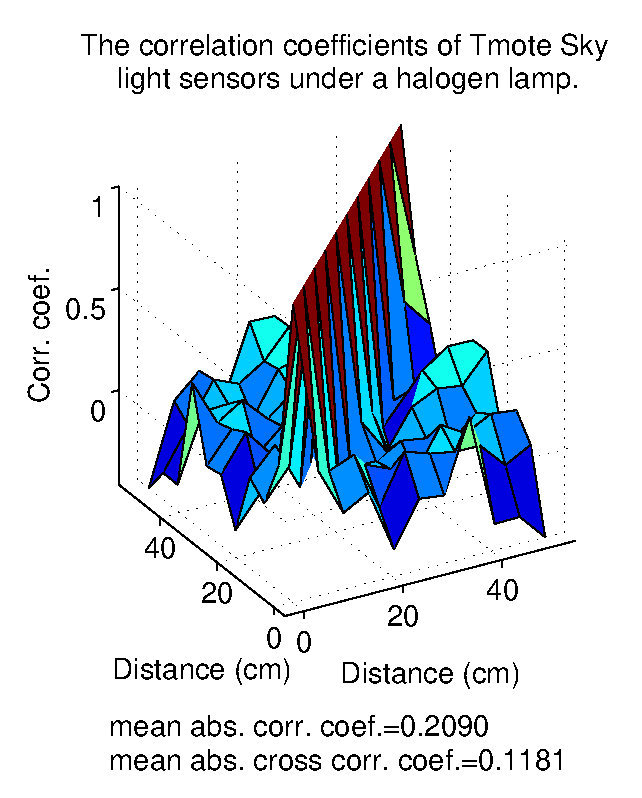
\includegraphics[width=\fwC]{img/HalogenCorrCoef}\\
%  \includegraphics[width=3.5cm]{img/ExpCorrCoef}\\
  \caption{The correlation coefficients of Tmote Sky light sensors. (Based on our hardware experiment data.)}\label{f:sensorIID}
\end{figure}


Sensor selection can be discussed within the framework of optimal estimation, where the estimation error is normally used as the cost function of the optimization. In previous works~\cite{SAM2006Amit,Fusion2005Amit,JafariGASensorSelectionInformationSciences2001} and~\cite{UcinskiPatanDoptSensorSelection06}, the sensor selection problem is formulated as a constraint 0-1 integer programming problem, where the estimation error is minimized. The number of sensor is given and used as the constraints. In~\cite{SAM2006Amit}, the sensor selection is formulated as a 0-1 integer programming (or binary integer programming) problem and solved by a branch and bound (B\&B) method. In~\cite{JafariGASensorSelectionInformationSciences2001}, the sensor selection problem is formulated as a combinatorial optimization problem as well as a binary integer programming problem. The problem is solved by a GA (genetic algorithm) software.
 Those methods are closest to our proposed method, but the difference is still obvious: Our method does not explicitly minimize or choose the number of selected sensors.


Our method is an example of the implicit optimization. The feature of this class of methods is that the number of selected sensors is not explicitly shown in the cost function or constraints of the optimization. Instead, the number of selected sensors is minimized simultaneously during the time when estimation error is minimized. It is desirable and may be counter-intuitive. Using the minimum number of sensors, the least estimation error can be achieved! Selecting more sensors does not necessarily improve the estimation precision. Rather, more properly scheduled sensors can cover a larger area for observation. Before presenting the details in Section~\ref{s:problemsolution}, we summarize the key features of our method: (1) Simultaneously achieve the optimal estimate with the least number of sensors, as well as the least energy costs. No compromise is required between the estimation precision and energy cost. (2) Simple and fast. (3) The robustness of the method has been verified by extensive hardware experiments.


\subsection{Overview on Our Strategy}\label{s:big}
    As aforementioned, the sensor selection problem is NP hard. Thus, our strategy is to simplify the problem by several reasonable approximations and solve the approximated problem by a fast optimization approach.


     We do not add the two cost functions (cost for estimation errors and number of selected sensors) together and minimize the summation, or construct a vector based on the cost functions. These are standard multi-objective or combinatorial optimization techniques. Instead, we only minimize the cost function that associated with the estimation error. However, the number of selected sensor is automatically minimized during the time when we minimize the estimation error. This is due to the fact that we intentionally select a proper convex cost function and it has a convex constraint. According to the Carath\'{e}odory's theorem, the number of selected sensors is minimized. The details are presented in the Section~\ref{s:analysis}.


% In short, we want to kill two birds with one stone. That is, we want to approach both the lowest estimation error bound, which is limited by Cram\'{e}r-Rao lower bound (CRLB) in theory, and the minimum number of selected sensors that allowed by the Carath\'{e}odory's theorem.


  We do not add the two cost functions (cost for estimation errors and number of selected sensors) together and minimize the summation, due to the high computation cost of integer programming. Remind that the number of selected sensors is an integer.  Thanks to the gradient, the computation costs of continuous optimization problems are normally much less than the of the integer programming problems.
  %   Normally, the computation cost to minimize an integer cost function is much higher than that of continuous cost function.
  % It will take much more computations to minimize that cost function than our proposed, continuous cost function.


The system block diagram of our proposed method is shown in Fig.~\ref{fig:sysmodel}, where the physical parameter $\mathbf{q}^\ast$ is the position of lamp, $y_{i}$ is the nominal light value, $v_{i}$ is the sensor measurement noise, and $s_{i}$ is the sensor reading.
    Note that our convex optimal sensor selection (COSS) algorithm includes the three blocks on the right, i.e., ``wireless sensor network,'' ``least squares fitting,'' and ``optimal sensor selection.'' As we can see in Fig.~\ref{fig:sysmodel} that the three blocks interact on each other, and they are inter-dependent. Thus, all the blocks are included in our COSS algorithm, which is list in Algorithm~\ref{a:COSS}, Section~\ref{s:solution}. The ``wireless sensor network'' is associated to part 1 of the Algorithm~\ref{a:COSS} and carried out on individual sensor node. The part 2 in the Algorithm~\ref{a:COSS} is referring to the other two blocks, i.e., ``least squares fitting,'' and ``optimal sensor selection,'' in Fig.~\ref{fig:sysmodel}. The part 2 is the task for the sink.

\begin{figure*}
\begin{center}\includegraphics[%
%  width=\linewidth,
  width=\fwA,
  keepaspectratio]{img/CentEDSysBlock}\end{center}
\caption{System block diagram of the proposed method.\label{fig:sysmodel}}
\end{figure*}


% In this system architecture, the WSN is not a passive sensing device. The sampling rate of the WSN is adapted according to the estimate $\mathbf{\hat{q}}$. The sensors and the sink interactively adjust the sampling rate for optimal estimation.
% After actively adjust its sampling rate, the data collected by the WSN is changed, which future affect the estimate $\mathbf{\hat{q}}$. Thus, if the system continuously updates the sample rate value, it is essentially a closed-loop control problem, and the stability must be guaranteed. In this


The future working scenario is shown in Fig.~\ref{f:scenario}.
In the figure, a target tracking scenario is demonstrated. However, the
method is applicable to generic parameter estimation problems.
After a target appears on the field of view, a subset of
the sensor nodes observe the event and start measuring the
physical quantity (light, temperature, gas concentration etc)
that is associated with the target. At the beginning, many
the sensor nodes detect the target and they enter an active mode.
Their sampling rates and transmission rates are levitated to a high level, as shown in Fig.~\ref{f:scenario}(A).
Although the transmission rate is high, not too much energy is
required, since this initial stage does not last for a long time.
    Soon, several sensors are selected to stay in the active mode
    and continuously monitor the target.
    Other sensors switch back to the inactive mode. Their sampling rates and transmission rates are considerably lower.
    One elected leader sensor among the
    active sensors takes the responsibility to report monitoring data to the sink.
    All these operations should be distributed, in future. This case is shown in
    Fig.~\ref{f:scenario}(B).
        As the target moves, the selected sensors smoothly shift from one to another. This
        is shown in Fig.~\ref{f:scenario}(C).
            Our current hardware implementation is presented in Section.~\ref{s:experiment}. Although the current implementation is not at the level of this future working scenario, the experiment indicates that the proposed COSS algorithm is fast and memory efficient. It has potentials to be implemented on low cost sensor nodes.
%Once data starts arriving at the sink, the
%rough position of the target can be estimated through a least squares
%optimization program running on the sink. Based on
%this rough position estimate, only some subset of sensor nodes are selected
%and continue to be assigned high sampling rates, while others are unselected
%and virtually stop sampling and packet transmission in order to conserve precious
%on-board battery energy. The process continuously refines
%the position estimate and then selecting different sensors based on the
%track of the target. This is shown in Fig.~\ref{f:scenario}(b).
%Note that, the same scheme can be adopted to estimate other
%target parameters. For example, in addition to the location of
%an illumination source, it might be required to estimate the
%strength of the illumination source as well. In future work,
%alongside the problem of sampling rate assignment, we plan
%to consider efficient routing of packets from sensor nodes to
%sink as shown in Fig.~\ref{f:scenario}(c).


\begin{figure*}
%\begin{center}\subfigure[A target appears.]{\includegraphics[%
%  width=0.3\linewidth,
%  keepaspectratio]{EventObs1.eps}}\subfigure[Select sensors.]{\includegraphics[%
%  width=0.3\linewidth,
%  keepaspectratio]{EventObs2.eps}}\subfigure[Sensor data are route to the sink.]{\includegraphics[%
%  width=0.3\linewidth,
%  keepaspectratio]{EventObs3.eps}}\end{center}
\centering
\includegraphics[width=\fwA]{img/COSSScenario}
\caption{The WSN sensor selection working scenario.\label{f:scenario}}
\end{figure*}

    As aforementioned, the original sensor selection problem has a large solution space and it is hard to solve. Thus, our strategy is to simplify the problem by several reasonable approximations and solve the approximated problem by a fast optimization approach.
% In short, we want to kill two birds with one stone. That is, we want to approach both the lowest estimation error bound, which is limited by Cram\'{e}r-Rao lower bound (CRLB) in theory, and the minimum number of selected sensors that allowed by the Carath\'{e}odory's theorem.


%\subsection{Background Knowledge:Fisher information}~\label{s:fi}
%%% moved to the appendix
%Fisher information is a metric to indicate the sensitivity of the measurements with respect to system parameters.
%%\begin{mdef}\label{d:fisher}
%%If a measurable random variable $X$ depends on parameter $\theta$, and the likelihood function is $l(\theta;X)$.
%%Then the Fisher information is
%%\begin{equation*}
%%    \mathcal{I}=E\{[\frac{\partial}{\partial \theta} \log l(\theta;X)]^2 \}
%%\end{equation*}
%%The matrix form is Fisher information matrix, which is $M$, with the $i,j$th entry defined as:
%%\begin{equation*}
%%    M_{(i,j)}=E\{\frac{\partial}{\partial \theta_i} \log l(\theta;X) \frac{\partial}{\partial \theta_j} \log l(\theta;X) \}
%%\end{equation*}
%%\end{mdef}
%
%Easy to see, if $P_r(X;\theta)$ is independent Gaussian, the sensitivity for each sensor can be computed separately.
%% Eq.~\ref{e:m} is the Fisher information matrix.
%\begin{eqnarray*}
%% \nonumber to remove numbering (before each equation)
%  l(\theta;X) &=& \frac{1}{\sqrt{2\pi}\sigma} \exp(-\frac{(X(\theta)-\mu)^2}{2\sigma^2})\\
%  M_{(i,j)} &=& E\{\frac{\partial}{\partial \theta_i} \log l(\theta;X) \frac{\partial}{\partial \theta_j} \log l(\theta;X) \} \\
%%  M_{(i,j)}&=& E\{\frac{\partial}{\partial \theta_i}(-\ln(\sqrt{2\pi\sigma^2})-\frac{(X(\theta)-\mu)^2}{2\sigma^2})
%%    \frac{\partial}{\partial \theta_j}(-\ln(\sqrt{2\pi\sigma^2})-\frac{(X(\theta)-\mu)^2}{2\sigma^2}) \}\\
%  M_{(i,j)} &=& E\{\frac{(X-\mu)^2}{\sigma^4}\frac{\partial X}{\partial \theta_i}\frac{\partial X}{\partial \theta_j} \} \\
%  M_{(i,j)} &=& \frac{1}{\sigma^2} \frac{\partial X}{\partial \theta_i}\frac{\partial X}{\partial \theta_j}
%\end{eqnarray*}
%Thus, (\ref{e:m}) is the Fisher information matrix.
%
%%A related concept is Fisher information entropy. Paper~\cite{RomeraFisherEntropy99} formulates Fisher information entropy for a 3D particle system as $\mathcal{I}_f$,
%%\begin{equation}\label{e:fentropy}
%% \mathcal{I}_f = \int [\|\nabla f(\mathbf{r})\|^2 /f(\mathbf{r}) ] \hbox{d}\mathbf{r},
%%\end{equation}
%%where $f(\mathbf{r})=f(x,y,z)$ is the pdf for a particle appears at the position $\mathbf{r}$.
%
%
%\begin{thm}[Cram\'{e}r-Rao inequality \cite{MoonSig} pp.551]
%If $t(\theta)$ is any unbiased estimator of $\theta$ based on a differentiable likelihood function, then
%\begin{equation} \label{e:crlb}
%    E\{(t(\theta)-\theta) (t(\theta)-\theta)^T\} \geq M^{-1}(\theta),
%\end{equation}
%where $M(\theta)$ is the Fisher information matrix (FIM).
%\end{thm}
%\begin{remark}
%According to this theorem, the inverse of the FIM is the indicator for the minimum possible covariance of any unbiased estimators. In fact, if the maximum likelihood estimator, $\theta_{ML}$, exists, the following equation holds~\cite{EmeryOED98}:
%$$E\{(\theta_{ML}-\theta)(\theta_{ML}-\theta)^T\}=M^{-1}(\theta). $$
%In other words, reducing the right hand side of (\ref{e:crlb}) actually improves the estimator $\theta_{ML}$, if it exists.
%%if we can find an unbiased estimator $\bar{t}(\theta)$ achieve the CRLB, or $ E\{(\bar{t}(\theta)-\theta) (\bar{t}(\theta)-\theta)^T\} = M^{-1}(\theta)$, then $\bar{t}(\theta)$ is called efficient.
%%    Although it is possible that a biased estimator has less error
%%If we have a
%\end{remark}



\subsection{Problem Formulation}\label{s:problemformulation}
% Our method follows the framework of experiment design and it is applicable to general parameter estimation problems, not just limited to the target tracking. However, for presentation purpose, we use a lamp tracking case has the example to interpret our formulation. This is the exact working scenario of our hardware testbed.

    Assuming the true position of the lamp at the time instance $k$ is $\mathbf{q^\ast}[k]$, and the position of the $i$th sensor is $\mathbf{r}_i$. The following equations hold:
\begin{eqnarray*}
    y_i[k] &=& f(\mathbf{q^\ast}[k]; \mathbf{r}_i), i=1,2,\cdots,n ;\label{e:yfq} \\
    s_i[k] &=& y_i[k]+v_i[k].\label{e:syv}
\end{eqnarray*}
where $f$ is the sensor model, $y_i[k]$ is the nominal reading from the $i$th sensor, and the associated real sensor reading is $s_i[k]$, which is corrupted by the independent Gaussian noise $v_i[k]$. In this chapter, we use a common energy model~\cite{ArandaOptSensorPlacement05} as the sensor model.


\begin{mdef}[Energy Model]
\begin{eqnarray}
% \nonumber to remove numbering (before each equation)
  y_i[k] &=& \frac{c_1}{h^2+d_i^2[k]}, \label{e:ynormal} \\
  v_{i}[k] & \thicksim & \mathcal{N}(0,\sigma),\nonumber \\
  d_i[k] &=& \| \mathbf{r}_i-\mathbf{q^\ast}[k] \| , \nonumber
\end{eqnarray}
  where $h$ is the height of the lamp, $d_i[k]$ is the distance from the sensor to the exact position under the lamp, $c_1$ is a constant, and $\sigma$ is the standard deviation.
\end{mdef}

\begin{remark}
The energy model can be reasonably interpreted by physics. The fact that the sensor can observe the target indicates there is energy come from the target being detected by the sensor. The energy emitted from the target is uniformly spread in space and propagates in spheres. Thus, the energy density is proportional to $1/r^2$, where $r$ is the radius of the sphere, or the distance from the target to the sensor. Under ideal conditions, if the sensor characteristics are linear, i.e., the sensor reading is proportional to the energy it received, then the energy model holds.

% The energy model is constructed based on physical properties. Fig.~\ref{f:EnergyModel}(a) illustrates why the nominal measurement is proportional to inverse of the distance square. The light bulb in Fig.~\ref{f:EnergyModel}(a) indicates a target which broadcast energy to the free space. A reasonable assumption is that the sensor's nominal measurement is proportional to the energy density. If the energy is emitted at a constant rate, then the summations of the energy on spheres of different radii are equal. Since the surface area of the sphere is $4\pi r^2$, the sensor's nominal measurement is $c_1/r^2$.


The configuration scenario of the energy model is shown in Fig.~\ref{f:EnergyModel}, where the target is on top of the plane that the sensor lay on. Easy to see that $r^2$ can be replaced by $h^2+d^2$. Thus, (\ref{e:ynormal}) is derived.

\begin{figure}
  \centering
%  \subfigure[Free space energy model.]{\includegraphics[width=4cm]{img/EnergySurf}}
%  \subfigure[Generic settings of energy model.]{\includegraphics[width=7cm]{img/LampEnergyModel}}
%  \caption{Configuration of energy model.}\label{f:EnergyModel}
  \includegraphics[width=7cm]{img/LampEnergyModel}
  \caption{Generic settings of energy model.}\label{f:EnergyModel}
\end{figure}


In the simulations of this chapter, we use the following constants
\begin{itemize}
  \item $c_1=3.3032\times 10^6$,
  \item $h=20.32$ cm.
\end{itemize}
\end{remark}
These parameters are chosen such that the energy model approximates the data measured by experiments.

\begin{mdef}[Polynomial Model]~\label{d:poly}
\begin{eqnarray*}
   y_i[k] &=& \left\{
  \begin{array}{ll}
    c_2 + c_3 d_i[k] + c_4 d_i^2[k], & \hbox{$y_i[k]\geq y_L$,} \\
    Invalid, & \hbox{otherwise,}
  \end{array}
\right.\\
  v_{i}[k] & \thicksim & \mathcal{N}(0,\sigma_i[k]),\\ %\label{eq:ynormal} \\
  \sigma_i[k] &=& \left\{
                    \begin{array}{ll}
                      c_5+c_6 d_i[k] + c_7 d_i^2[k], & \hbox{$y_i[k]\geq y_L$,} \\
                      Invalid, & \hbox{otherwise,}
                    \end{array}
                  \right. \\
  d_i[k] &=& \| \mathbf{r}_i-\mathbf{q^\ast}[k] \| ,
\end{eqnarray*}
where $c_2$ to $c_7$ are constants, and $d_i[k]$ is the distance from the sensor to the exact position under the lamp.
\end{mdef}
\begin{remark}
The polynomial model is characterized based on our hardware experiment data. The data are plot in Fig.~\ref{f:SensorFit}. The left plot in the figure is the light value with respect to the distance, measured by cm. While the right plot is the standard deviation with respect to the distance. Note that the value of the standard deviation depends on the distance, in practice. In the figure, it is seen that the fitting errors of the polynomial model are relatively small.

The experiment data can be fitted by the energy model. However, the fitting error is larger than that of the polynomial model. This may due to the nonlinear characterizes of the sensors.

In the hardware implementations, we use the following parameters:
\begin{itemize}
  \item \begin{tabular}{ccc}
          % after \\: \hline or \cline{col1-col2} \cline{col3-col4} ...
          $c_2=6720.0,$ & $c_3=-216.0,$ & $c_4=2.524,$ \\
        \end{tabular}
  \item $\; y_L=2500$,
  \item \begin{tabular}{ccc}
          % after \\: \hline or \cline{col1-col2} \cline{col3-col4} ...
          $c_5=824.0,$ & $c_6=-36.26,$ & $c_7=0.4577.$ \\
        \end{tabular}
\end{itemize}

In the model, ``invalid'' means that the optimization for sensor selection does not consider the invalid sensors. Just as if those invalid sensors are not exist. The $y_L$ is the threshold where the ambient light is more significant than the lamp's light. In Fig.~\ref{f:SensorFit}, $y_L$ is about 35 cm.
\end{remark}

\begin{figure}
  \centering
%  \subfigure{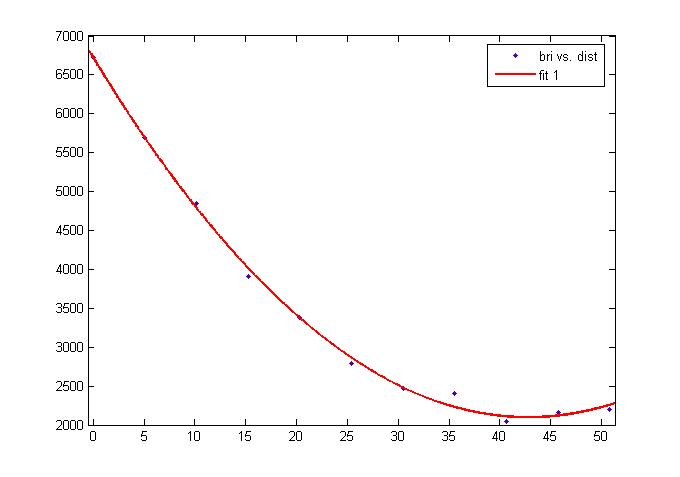
\includegraphics[width=6cm, height=6cm]{img/SensorFit2DOct02Quad}} %
%  \subfigure{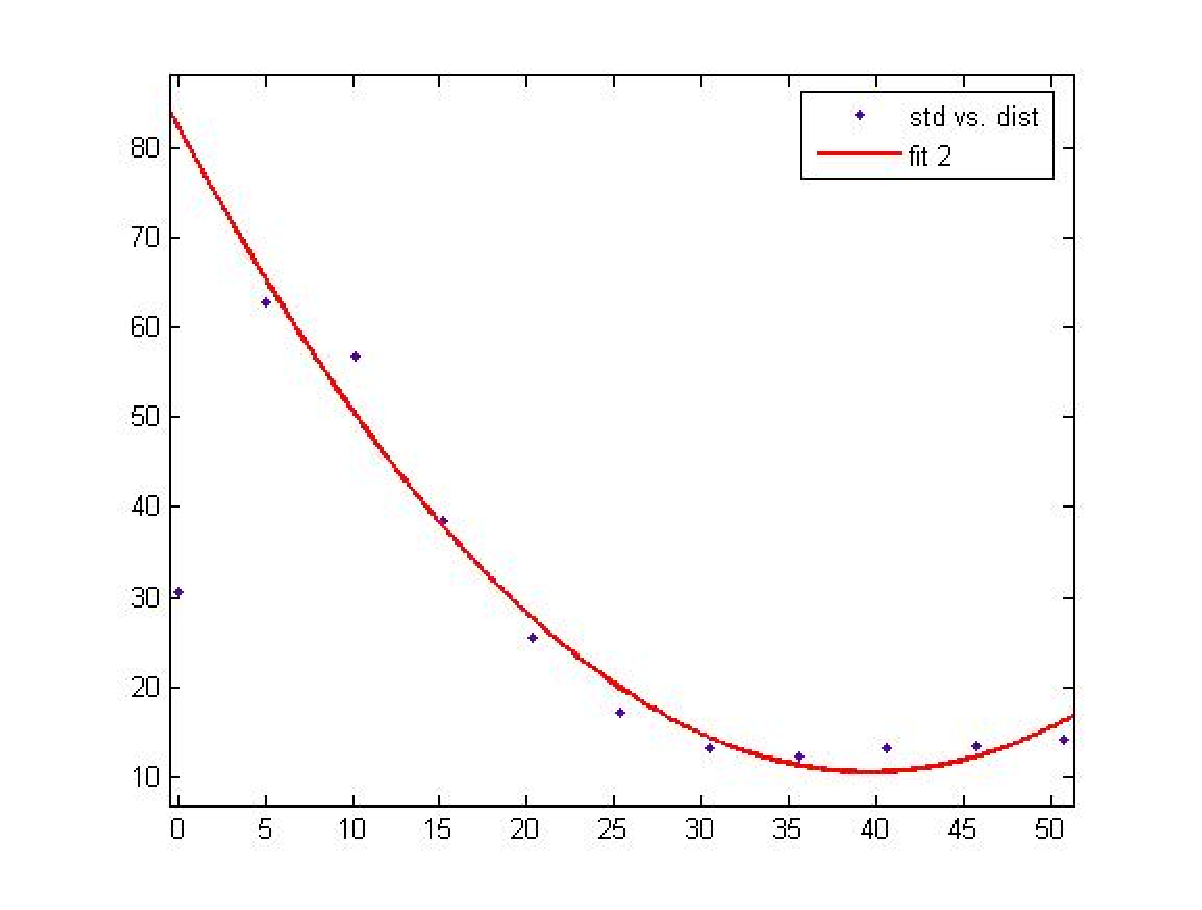
\includegraphics[width=6cm, height=6cm]{img/SensorFit2DOct02StdQuadRobust}}
  \subfigure{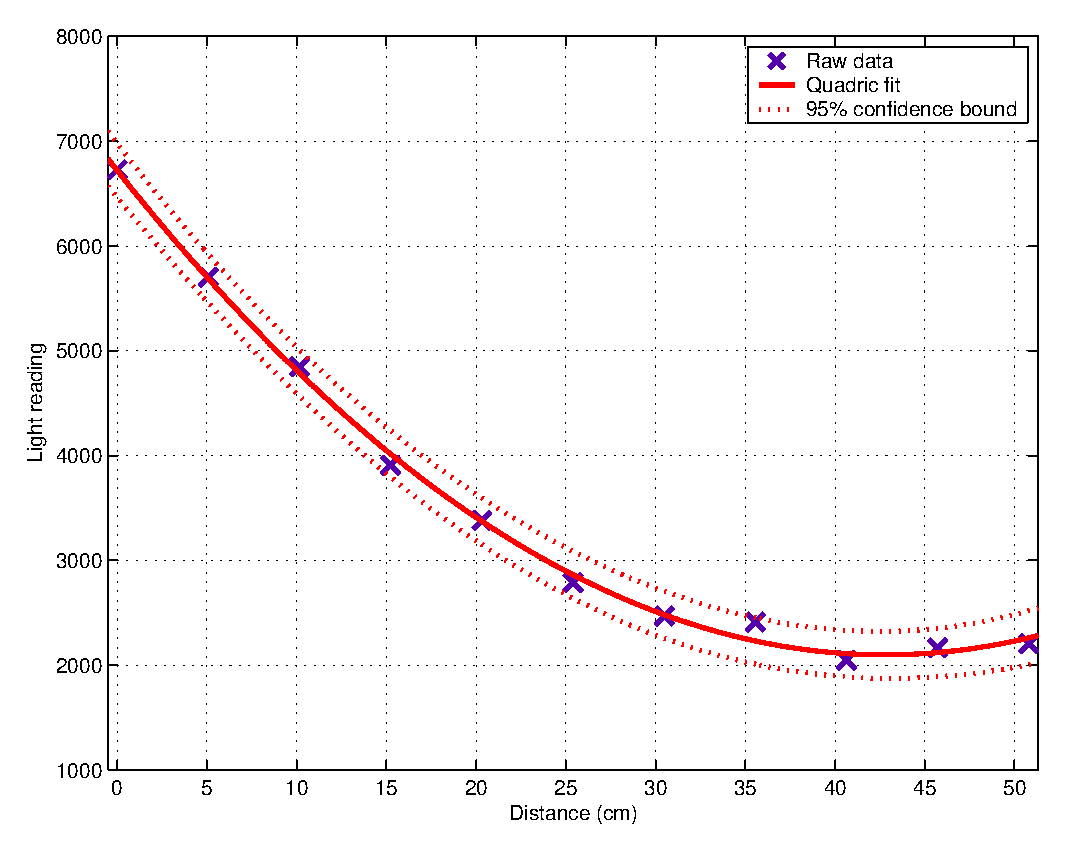
\includegraphics[width=6cm, height=6cm]{img/RangeLightFit}}
  \subfigure{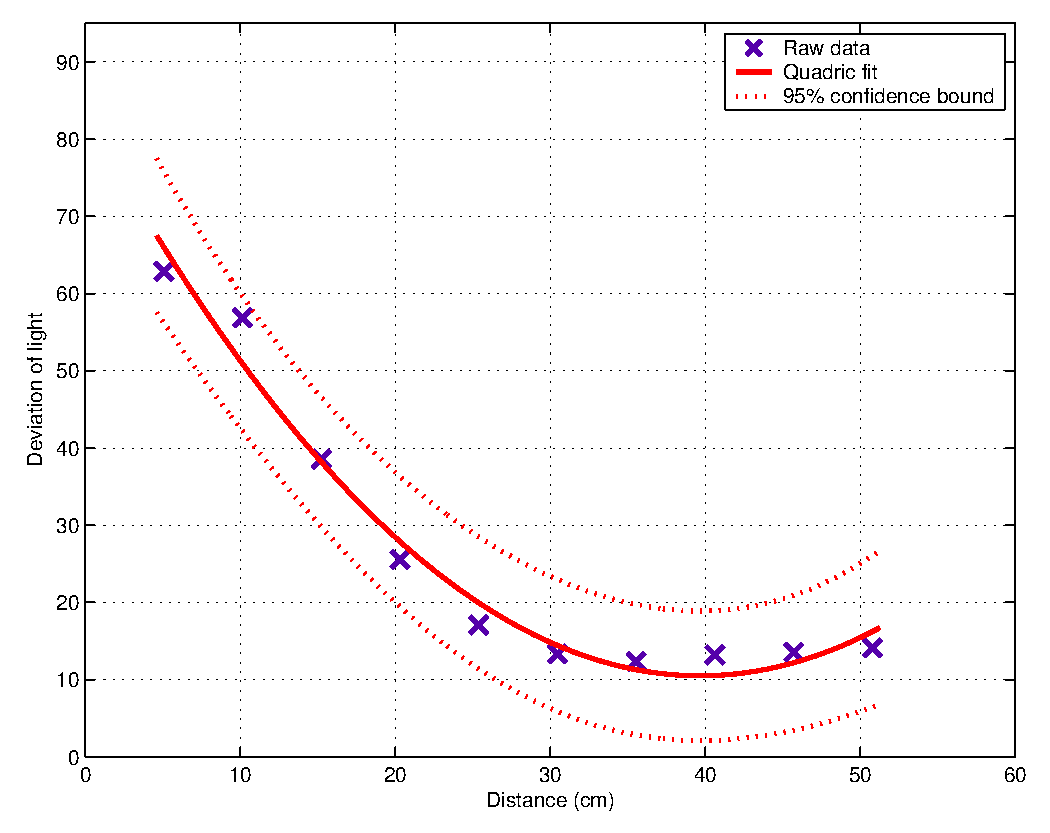
\includegraphics[width=6cm, height=6cm]{img/RangeStdFit}}
  \caption{The characteristics of the light sensors on Tmote Sky.}\label{f:SensorFit}
\end{figure}


In order to reduce the noise $v_i$, the $i$th sensor node measures the $n_i$ light values in the time slot $t_S$, averages them and sends the averaged value back to the sink. The averaged light value is $\bar{s}_i[k]$, whose standard deviation is smaller than that of the raw data:
$$\bar{\sigma}_i^2[k]=\sigma_i^2[k]/n_i.$$
 If we can afford infinite number of samples, we can reject the noise totally. Of course, there is an upper limit on sample number in practice. For simplicity, we set $n_S$ as the upper limit on the total number of samples for all the sensors in the time slot $t_S$.
    The intuitive interpretation is as follows.
We estimate the position of an event based on sensor measurements.
Since sensor measurements are noisy, the event observations are not perfect.
Now, noise in the sensor measurements can be reduced by modifying the sensor design (use better hardware) or by filtering
away sensor noises. Given fixed hardware, a simple filtering technique to adopt is to average the sensor data.
%In the latter approach, one possible option is to take a large number of sensor measurements (samples) and then average them by each sensor to eliminate as much noise as possible.

After receiving all the sensor data, the sink estimates the lamp's position by the standard nonlinear least squares (LS) method, and the output is $\hat{\mathbf{q}}_A$, which is also called the a priori position. For a network of $n$ sensors, the $\hat{\mathbf{q}}_A$ is as (\ref{e:qA}).
\begin{equation}\label{e:qA}
    \hat{\mathbf{q}}_A[k] = \mathrm{argmin}_{\mathbf{q}} \frac{1}{2} \sum_{i=1}^{n} (\bar{s}_i[k]-y_i(\mathbf{q}; \mathbf{r}_i))^2.
\end{equation}



Now, we introduce several approximations to simplify the problem.
\begin{itemize}
  \item Instead of assigning each sensor a binary value that indicates the ``selected'' or ``unselected'' state, we assign a normalized sampling rate $p_i$ to sensor $i$. That is, $$p_i[k]\in [0,1] \;\mathrm{ and } \sum_i p_i=1.$$ Thus, the integer programming problem is approximated by a continuous design problem.
       \item Our cost function is based on the Fisher information matrix (FIM), $M$, whose inverse matrix is the Cram\'{e}r-Rao lower bound (CRLB)~\cite{CheungLSTOA04,UcinskiOptDPS05}.
   The definition of Fisher information and FIM is presented in Appendix.~\ref{s:fi}.
    Ideally, the optimal sampling rate is
    $$\mathbf{p}^\ast[k]=\mathrm{argmin}_{\mathbf{p}} \Psi(M(\mathbf{p};\mathbf{q}^\ast[k])).$$ Since $\mathbf{q}^\ast[k]$ is unknown, we replace it by $\hat{\mathbf{q}}_A[k]$, which is another approximation. Thus, $$\hat{\mathbf{p}}[k]=\mathrm{argmin}_{\mathbf{p}} \Psi(M(\mathbf{p};\hat{\mathbf{q}}_A[k])).$$
        \item The nonlinear sensor models are linearized as $\mathbf{y}[k] = A^T \hat{\mathbf{q}}_A[k].$ This is a common approximation technique.
\end{itemize}
Thus, we simplified the original problem to the following sampling rate optimization problem.
\begin{mdef}[Sampling Rate Optimization Problem]\label{d:SampRateOpt}
\begin{eqnarray}
 \hat{\mathbf{p}}[k]  &=&  \mathrm{argmin}_{\mathbf{p}} \Psi(M(\mathbf{p}; \mathbf{\hat{q}}_A[k])),  \label{e:pk}\\
% \Psi(M) &=& -\ln\det(M), \label{e:dopt}\\
 \hbox{\rm subject to} :  \mathbf{p} &\geq& 0 ,  \nonumber \\
 \mathbf{1}^{T}\mathbf{p} & = & 1 , \nonumber \\
 \mathbf{y}[k] &=& A^T \hat{\mathbf{q}}_A[k],\nonumber \\
 A &=&  \nabla_{\mathbf{q}}\mathbf{y}|_{\mathbf{q}=\mathbf{\hat{q}}_A[k]}, \label{e:defA} \\
 M &=&  A \Sigma^{-1}A^T , \label{e:mSSP}\\
 \Sigma^{-1} & =& \left[\begin{array}{ccc}
        \tilde{\sigma_{1}}^{-2}[k] & 0\\
        0 & \tilde{\sigma_{2}}^{-2}[k] \\
        &  & \ddots\end{array}\right], \nonumber
 \end{eqnarray}
\end{mdef}
where $\tilde{\sigma_{i}}[k]$ is model dependent:
\begin{itemize}
\item For energy model: $\tilde{\sigma_{i}}^{-2}[k] = \sigma^{-2} p_{i}[k]$,
\item For polynomial model: $\tilde{\sigma_{i}}^{-2}[k] = \sigma_i^{-2}[k] p_{i}[k]$.
\end{itemize}
The definition of $\Psi(M)$ follows (\ref{e:dopt}).
\begin{equation}\label{e:dopt}
\Psi(M) = -\ln\det(M).
\end{equation}



%Eq.~\ref{e:dopt} is called the D-optimum criterion in the literature of experiment design.
A natural question to ask is why the $\Psi$ function is defined as (\ref{e:dopt}). This function is called D-optimality criterion in the literature of optimal experiment design (OED)~\cite{EmeryOED98}. In order to define the cost function as a scalar, the matrix $M$ should be ``scalarized'' to a real number that indicates the ``size'' of the matrix. The D-optimality criterion is one but not the unique choice.
%Another ``scalarization'' function is valid as far as the following requirements are satisfied:
%\begin{itemize}
%  \item $\Psi(M)$ is strictly convex for valid $M$.
%  \item All possible values of $M$ construct a convex set.
%  \item $\Psi(M)$ a real number.
%\end{itemize}
Of course, if $\Psi(M)$ is also differentiable, then the optimization is easier.

Remember that $\det(M)$ is the volume of matrix $M$. Actually, when $M$ is a 3 by 3 matrix, $\det(M)$ is the volume of the parallelepiped constructed by the three column vectors of $M$. In other words, $\det(M)$ is a metric to measure the size of $M$. Since $\det(M^{-1})=1/\det(M)$, $\det(M^{-1})$ is minimized when $-\ln\det(M)$ is minimized.

Commonly used optimality criteria include:
\begin{itemize}
  \item The D-optimality criterion: $\Psi(M)=-\ln\det(M)=\ln\det(M^{-1})$. %\footnote{It is also defined as $\det(M)^{1/k}$. Easy to see that the two definitions of the D-optimality criteria are equivalent.}
  \item The E-optimality criterion: $\Psi(M)=-\lambda_{\max}(M^{-1})$.
  \item The A-optimality criterion: $\Psi(M)=-\hbox{tr}(M^{-1})$.
%  \item The T-optimality criterion: $\Psi(M)=\hbox{trace}(M)$.
\end{itemize}
Even though there are other optimality criteria available, D-optimality criteria is more commonly used. The unique feature of D-optimization compared to the rest is
that the result of the D-optimization is not affected by linear transforms. That is, the result of the D-optimization is not affected by whether the unit of the measurements is in centimeters or in inches. In addition, the D-optimality criteria is differentiable. The computation on D-optimization is easier than that for E-optimization, which is not differentiable.
    Although different optimality criteria may lead to significant different result, when $M$ is not close to singular, the result of different optimality criteria are often close to each other. The details are presented in Section.~\ref{s:geo}
    %An example is shown in~\cite[pp.389]{Boydcvxbook}.




Now we prove that the FIM, $M$, is the inverse of the covariance of estimation error $\mathbf{e}$.

\begin{thm}\label{t:invM}%[Estimation of covariance matrix]
   For the linear system $\mathbf{s}=A^T \mathbf{q}^\ast + \mathbf{v}$, where $v_i$ is a zero mean noise with a standard deviation of $\sigma_i$, we have $M^{-1}$ equals the covariance matrix of the estimation error. That is
   $$cov(\mathbf{e}) = M^{-1},$$ where $M=A\Sigma^{-1}A^T,$ $\mathbf{e}=\mathbf{\hat{q}}-\mathbf{q}^\ast$ and $\mathbf{\hat{q}}$ is an unbiased estimator of $\mathbf{q}^\ast$. $\mathbf{\hat{q}}$ is defined as
   $\mathbf{\hat{q}}= \mathrm{argmin} (A\mathbf{q}-\mathbf{s})^T\Sigma^{-1}(A\mathbf{q}-\mathbf{s}).$
\end{thm}

\begin{proof}
    It is well known that $\mathbf{\hat{q}}=(A\Sigma^{-1} A^T)^{-1}A\Sigma^{-1}\mathbf{s}$.  %    if the cost function of weighted LS (WLS) estimation~\footnote{It is proved that the $\mathbf{\hat{q}}$ computed based on this WLS cost function is better than LS, in the sense that it is closer to CRLB than the LS cost function. The weight $\Sigma$ is optimal ~\cite{CheungLSTOA04}.} is $\mathcal{J}=\min (A\mathbf{q}-\mathbf{s})^T\Sigma^{-1}(A\mathbf{q}-\mathbf{s})$.
  Because $\mathbf{\hat{q}}$ is unbiased, $E\{\mathbf{\hat{q}}\} = \mathbf{q}^\ast$.
\begin{eqnarray*}
 cov(\mathbf{e}) & = & E\{ (\mathbf{e}-E\{\mathbf{e}\})(\mathbf{e}-E\{\mathbf{e}\})^T\} \\
 &=& E\{(\mathbf{\hat{q}}-\mathbf{q}^\ast-0)(\mathbf{\hat{q}}-\mathbf{q}^\ast-0)^T \} \\
 &=& cov(\hat{\mathbf{q}}) \\
 &=&E\{(M^{-1}M\mathbf{q}^\ast + M^{-1}A\Sigma^{-1} \mathbf{v} -  \mathbf{q}^\ast) \\
    &&(M^{-1}M\mathbf{q}^\ast + M^{-1}A\Sigma^{-1} \mathbf{v} -  \mathbf{q}^\ast)^T \} \\
 &=& M^{-1}A\Sigma^{-1} E\{\mathbf{v}\mathbf{v}^T\} \Sigma^{-T} A^T M^{-1}\\
 &=& M^{-1}.
\end{eqnarray*}
    In summary, $cov(\mathbf{e}) = M^{-1}$.
\end{proof}

Since $M^{-1}$ equals to the CRLB~\cite{CheungLSTOA04,UcinskiOptDPS05}, and $\Psi=\ln\det(M^{-1})$, the (\ref{e:pk}) minimizes the estimation error and pushes down the estimation error close to the CRLB.


%  It is known that, under certain assumptions the D-optimization has a ``sensor clustering'' effect~\cite{UcinskiOptDPS05}, i.e., after the optimization, most sensors have sampling rates close to 0. In the current literature, this effect is considered undesirable, and
%  different methods have been proposed to compensate this effect~\cite{fedorov-design96}. However, we notice that this effect is ideal for our sensor selection purpose.

Due to Theorem~\ref{t:minsen}, which will be presented later, after the optimization, most sensors have sampling rates close to 0. No more than $m(m+1)/2$ sensors have higher sampling rates, where $m$ is the number of parameters under estimation. Thus, we select sensors whose sampling rates are higher than a threshold $h_S$. The set of selected sensor is $\mathbb{S}_S$.
\begin{equation*}\label{e:ss}
    \mathbb{S}_S [k] = \{i| \hat{p}_i[k] \geq h_S \}.
\end{equation*}

It is not difficult to tune the $h_S$ in practice. Once (\ref{e:ss}) is finished, the sink turns off the sensors that have not been selected and collects the data from those selected sensors. Finally, the so called a posteriori position of lamp is estimated by the LS method.
\begin{equation*}\label{e:qB}
    \hat{\mathbf{q}}_B[k] = \mathrm{argmin}_{\mathbf{q}} \frac{1}{2} \sum_{i\in \mathbb{S}_S [k]} (\bar{s}_i[k]-y_i(\mathbf{q}; \mathbf{r}_i))^2.
\end{equation*}

The system keep estimating the lamp by the selected sensors, until at certain time, $k+i$, when the a posterior position estimate, $\hat{\mathbf{q}}_B[k+i]$, has a big error, then we restart from the a priori estimation again. The error bound of $\hat{\mathbf{q}}_B[k+i]$ is estimated by its associated FIM, $M_B[k+i]$.
\begin{eqnarray}
 A_B &=&  \nabla_{\mathbf{q}}\mathbf{y}|_{\mathbf{q}=\mathbf{\hat{q}}_B[k]}, \label{e:defAB} \nonumber \\
 M_B &=&  A_B \Sigma^{-1}A_B^T . \label{e:mb}
\end{eqnarray}


In fact, if the target is smoothly moving, we can also restart from the sampling rate optimization. That is, just choose another 3 proper sensors to observe the lamp, instead of turning on all the 15 sensors and then select 3 sensors out of the 15. This strategy is more energy efficient. However, this approach has a limit on the dynamic of the target, i.e., the target can not move too fast. In the current scenario, the dynamic of target is assumed unknown. For the worst case, a target may shift from one side of the field of view to the other side in no time. The above strategy, although may cost more energy, is capable to capture the target's position under the worst cases: When the lamp is suddenly shifted from one side to the other side.
    For some applications, since the target is smoothly moving, it is desirable to consider the target dynamics for better estimation precision. This is our future work.


\subsection{The Algorithm of the Convex Optimal Sensor Selection (COSS)}\label{s:solution}
    Definition~\ref{d:SampRateOpt} is formulated as an optimal experiment design problem, which can be solved by a multiplicative algorithm that updates $p_{i}[k+1]$ as $p_{i}[k]\phi_{i}(\mathbf{p}[k])/m$, where $\mathbf{\phi}(\mathbf{p}[k])=\nabla_{\mathbf{p}} \Psi.$ It is proved that this method is a solution of the D-optimality criterion~\cite{UcinskiOptDPS05,PazmanOED86}. We use this method as a part of our convex optimal sensor selection (COSS) algorithm, which is listed as Algorithm~\ref{a:COSS}. The computation of the algorithm is separated on the sensors and the sink.


\begin{table}
\caption{Convex Optimal Sensor Selection (COSS) Algorithm}\label{a:COSS}
\begin{algorithm}[H]
\vskip2mm
%\small
{\bf Part 1: On-sensor computation.}\\
\framebox[0.95\textwidth]{
    \begin{algorithm}[H]
Receive $t_S$ and $n_i$ from the sink\;
Collect $n_i$ samples in the time slot $t_S$, and $\bar{s}_i$ is the average of those samples\;
Wait for a small random time, then send $\bar{s}_i$ to sink\;
    \end{algorithm}
}
\vskip3mm
{\bf Part 2: On-sink computation.}\\
\framebox[0.95\textwidth]{
    \begin{algorithm}[H]
    \SetNoline
Initially $p_{i}=1/n$ and \texttt{State}$\leftarrow$\texttt{selection}\;
\If{\texttt{State}=\texttt{selection}}
{
    Send $n_{i}$, $t_S$ to the $i$th sensor\;
    Wait for time $t_S$, collect $\bar{s}_{i}$\;
    Estimate parameter $\mathbf{q}^\ast$ by the LS method, and the result is $\mathbf{\hat{q}}_A$\;
    \While{true}
        {
            \eIf{$\phi_{i}(\mathbf{p}[k+1])<m+\eta, i=1,2,\cdots,N$}
            {%then
                  exit the while loop\;
            }
            {%else
                $p_{i}[k+1]=p_{i}[k]\frac{\phi_{i}(\mathbf{p}[k])}{m}$ \;
            }
        }
        \lIf{$p_{i}[k+1]\geq h_S$}{$n_{i}=p_{i}[k+1]\times t_S$}~\lElse{$n_i=0$}\;
        Send $\mathbf{n}$ to the proper sensors and \texttt{State}$\leftarrow$\texttt{tracking}\;
}


\If{\texttt{State=tracking}}
{
    \While{true}
    {
        Wait for time $t_S$, collect sensor reading $\bar{s}_{i}$, $i\in \mathbb{S}_S$\;
        Estimate parameter $\mathbf{q}^\ast$ by the LS method. The result is $\mathbf{\hat{q}}_B$ and its associated FIM is $M_B$\;
        \lIf{$\Psi(M_B)$ is big}{\texttt{State}$\leftarrow$\texttt{selection}, exit the while loop\;}
    }
}

\end{algorithm}
}
\vskip2mm
\end{algorithm}
\end{table}


\subsection{Analysis on the Solution}\label{s:analysis}
Let us start from several definitions.
% The definition on convex set is not unique, though they are equivalent.

%\begin{mdef}[Convex set, based on \cite{BertsekasNP99}pp.557]
%Let $\mathbb{S}_C$ be a subset of $\mathbb{R}^n$. We say that $\mathbb{S}_C$ is convex if
%$$\alpha \mathbf{x}+(1-\alpha) \mathbf{y} \in \mathbb{S}_C, \forall \mathbf{x}, \forall\mathbf{y}, \mathrm{and\ } \mathbf{x},\mathbf{y}\in \mathbb{S}_C, \forall  \alpha\in [0, 1]. $$
%\end{mdef}

\begin{mdef}[Convex function] %, based on \cite{MoonSig}pp.860]
A function $f:\mathbb{S} \mapsto \mathbb{R}$ is called convex over an open set $\mathbb{S}$ if
$$ f(\alpha \mathbf{x} + (1-\alpha) \mathbf{y}) \leq \alpha f(\mathbf{x}) + (1-\alpha)f(\mathbf{y}), \forall \mathbf{x}, \forall\mathbf{y}, \mathrm{and\ } \mathbf{x},\mathbf{y}\in \mathbb{S}_C, \alpha \in [0, 1]. $$
The function is called strictly convex if the $\leq$ sign is replaced by $<$.
\end{mdef}

\begin{mdef}
The solution domain is $\mathbb{S}_P$, which is a simplex defined as
$$ \mathbb{S}_P = \{ \mathbf{p} |  \mathbf{p} \in\mathbb{R}^n, \mathbf{1}^T \mathbf{p}=1 , \mathbf{p} \geq 0 \} .$$
\end{mdef}


\begin{mdef}
Define the set of all possible FIM with
the unified sampling rate as the set $\mathbb{S}_{M}$. That is, $$
\mathbb{S}_{M}=\{ M|\sum_{i=1}^{n}\mathbf{p}_{(i)}\mathbf{a}_{i}\mathbf{a}_{i}^{T},
\mathbf{a}\in\mathbb{R}^{m}, \mathbf{p}\in\mathbb{S}_P \}.$$
\end{mdef}

Next, we present an important result, which is the foundation of Theorem~\ref{t:minsen}.

\begin{lem}\label{t:outofmin}
For the sampling rate optimization problem in Definition~\ref{d:SampRateOpt}, if $Rank(A)=m$, the gradient is not zero inside $\mathbb{S}_p$. That is, $\nabla_{\mathbf{p}} \Psi(M) \neq \mathbf{0}$, $\mathbf{p}\in \mathbb{S}_P$.
\end{lem}

\begin{proof}
% We are going to show that $\nabla_{\mathbf{p}} \Psi(M) \neq 0$ when $\sum_i p_i=1$, and $\| \mathbf{p} \|$ is finite. Then, it is impossible for the gradient to be equal to $0$ within the simplex $\mathbf{1}^T \mathbf{p}=1, \mathbf{p}\geq 0$.
For simplicity, we ignore the time index $[k]$ in this proof. For simplicity, define $\mathbf{a}_i$ as $A^T=[\mathbf{a}_1, \mathbf{a}_2, \cdots, \mathbf{a}_n]$. Remind that $A^T\in \mathbb{R}^{m\times n}$, and $A$ is defined in (\ref{e:defA}). So
\begin{eqnarray*}
\Psi(M) &=& -\ln\det(\sum_{i=1}^{n}p_i \mathbf{a}_i \mathbf{a}_i^T). \\
\frac{\partial \Psi(M)}{\partial p_j} &=& - tr(M^{-1} \mathbf{a}_j \mathbf{a}_j^T),\\
\frac{\partial \Psi(M)}{\partial p_j} &=& - \mathbf{a}_j^T M^{-1} \mathbf{a}_j, \\
\nabla_{\mathbf{p}}\Psi(M) &=& \left(
                                 \begin{array}{c}
                                   - \mathbf{a}_1^T M^{-1} \mathbf{a}_1 \\
                                   - \mathbf{a}_2^T M^{-1} \mathbf{a}_2  \\
                                   \vdots \\
                                   - \mathbf{a}_n^T M^{-1} \mathbf{a}_n  \\
                                 \end{array}
                               \right).
\end{eqnarray*}
We now show that there exists some positive $\partial\Psi(M)/\partial p_j$.


Firstly, $M$ is positive definite.
    To show this, we choose any $\mathbf{v}\in \mathbb{R}^m, \mathbf{v}\neq \mathbf{0}$, and multiply them to both sides of $M$
\begin{eqnarray*}
% \nonumber to remove numbering (before each equation)
  \mathbf{v}^T M \mathbf{v} &=& \sum_i p_i (\mathbf{v}^T \mathbf{a}_i)^2.
\end{eqnarray*}
Since $Rank(A)=m$, or full rank, we have $Null(A^T)=\varnothing$. Thus, there does not exist a $\mathbf{v}\in \mathbb{R}^m, \mathbf{v}\neq \mathbf{0}$, such that $\mathbf{v}^T \mathbf{a}_i=0$ for $\forall i\in [1, n]$. Or, $\mathbf{v}^T \mathbf{a}_i\neq 0$ for any $\mathbf{a}_i$.

In addition, since $\sum_i p_i=1$, and $p_i \geq 0$, there is at least one positive $p_i$. That is, $p_k > 0$. Then
$$p_k (\mathbf{v}^T \mathbf{a}_k)^2 > 0.$$
    For other $i\neq k$, we have
    $$p_i (\mathbf{v}^T \mathbf{a}_i)^2 \geq 0.$$
     So, $$\sum_i p_i (\mathbf{v}^T \mathbf{a}_i)^2>0.$$

Thus, $\mathbf{v}^T M \mathbf{v} > 0$, i.e., $M$ is positive definite.


Secondly, it is known that the inverse of a positive definite matrix is also positive definite.
    Since $Rank(A)=m$, there must exist $\mathbf{a}_i\neq \mathbf{0}$.
Because $M^{-1}$ is positive definite, for the none zero $\mathbf{a}_i$, i.e., $\mathbf{a}_i \in \mathbb{R}^m, \mathbf{a}_i\neq \mathbf{0}$, we have
$$\mathbf{a}_i^T M^{-1} \mathbf{a}_i > 0.$$


In summary, not all entries of $\nabla_{\mathbf{p}}\Psi(M)$ are equal to 0. Thus $\nabla_{\mathbf{p}}\Psi(M) \neq \mathbf{0}$.
\end{proof}


\begin{remark}
The geometric interpretation is shown in Fig.~\ref{f:outofmin}.
\begin{figure}
  \centering
  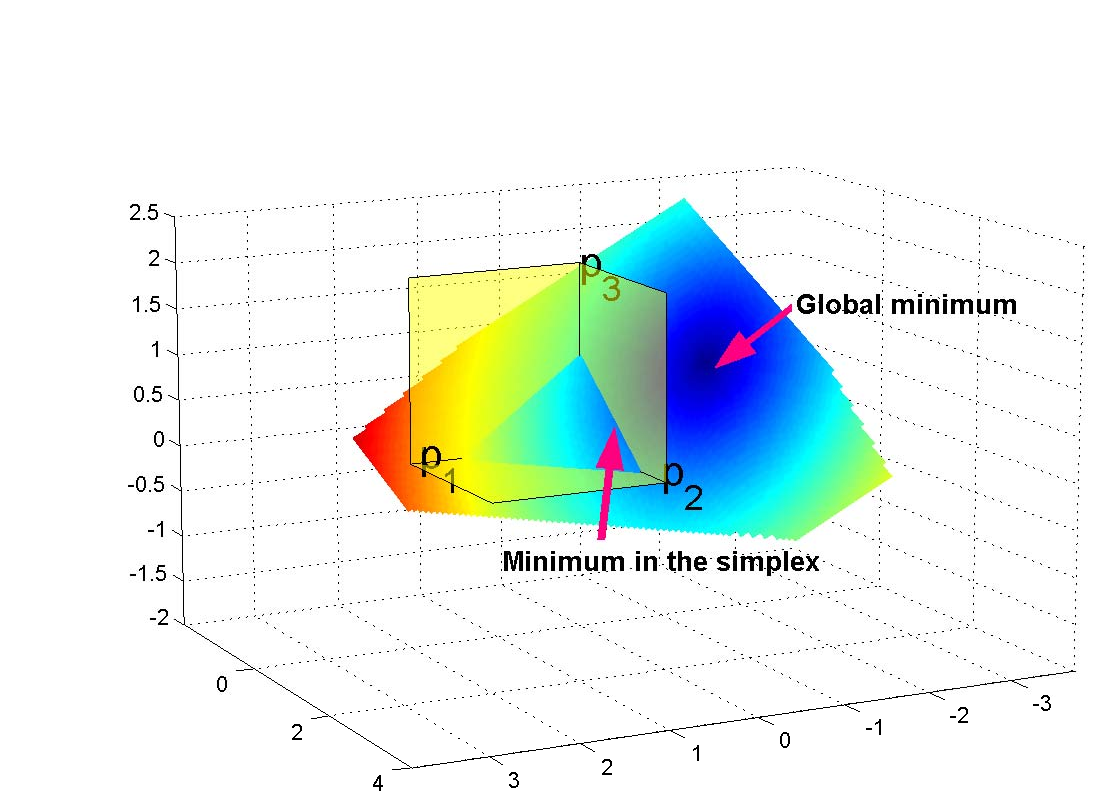
\includegraphics[width=\fwB]{img/CvxMinSimplex}
%  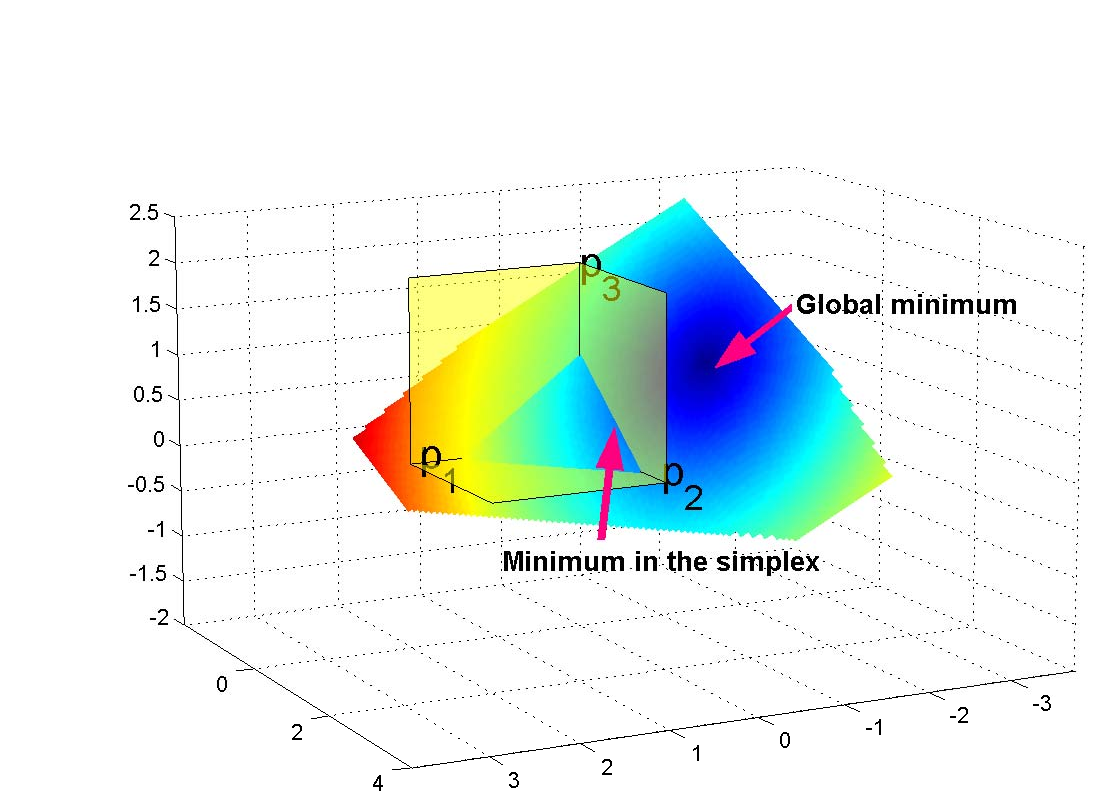
\includegraphics[width=\fwB]{img/CvxMinSimplex}
  \caption{A geometric interpretation on Lemma~\ref{t:outofmin}.}\label{f:outofmin}
\end{figure}
    In this 3D example, $p_1$, $p_2$ and $p_3$ are the axes. The parameter equation for the sliding surface is $p_1+p_2+p_3=1$. The simplex $\mathbb{S}_P$ is the triangle inside the $(p_1,p_2)$, $(p_2,p_3)$, and $(p_1,p_3)$ plans. The color of the sliding surface indicates the value of a cost function: The value of the cost function increases as the color changes from blue to red. The triangle is a convex set. If there exists a global minimum point with the gradient equals to $\mathbf{0}$ (stationary point), Lemma~\ref{t:outofmin} says that the global minimum point is out of the triangle, which is the same as Fig.~\ref{f:outofmin}. It is easy to see that the minimal value within the triangle, $\mathbb{S}_P$, must take place on the boundary of the triangle.


    Actually, for our sensor selection problem, the stationary point ($\nabla_{\mathbf{p}}\Psi = 0$) is infinite far away, where $\mathbf{p}\rightarrow \infty$ and $M^{-1} \rightarrow 0$. In other words, the estimation error is totally rejected if we take infinite number of samples.
    It is easy to see that the minimum value on the triangle must take place on the boundary of the triangle. While the 3D example is straightforward, we need to prove that such relations are still true for arbitrary high order.
\end{remark}

Next, we claim that $\mathbb{S}_M$ is convex for arbitrary high order. Since it is convex, the Carath\'{e}odory's theorem is valid on the set. Due to limited space, the proofs of several following theorems are ignored.

\begin{lem}\label{t:cvx}
$\mathbb{S}_M$ is a convex set.
\end{lem}
\begin{proof}
We want to prove the follows: if
$$M(\mathbf{p}_1)\in\mathbb{S}_{M}, M(\mathbf{p}_{2})\in\mathbb{S}_{M},$$
 and $$ \bar{M}=\alpha M(\mathbf{p}_{1})+(1-\alpha)M(\mathbf{p}_{2})$$ then $\bar{M}\in\mathbb{S}_{M}$,
where $\alpha\in\mathbb{R},\alpha\in[0,1]$.

Define $$\mathbf{p}_T := \alpha\mathbf{p}_1+(1-\alpha)\mathbf{p}_2.$$
If $$M(\mathbf{p}_{1})\in\mathbb{S}_{M} \mathrm{\ and\ } M(\mathbf{p}_{2})\in\mathbb{S}_{M},$$
then we have
\begin{eqnarray*}
\bar{M} & = & \sum_{i=1}^{n}\mathbf{p}_{T(i)}\mathbf{a}_{i}\mathbf{a}_{i}^{T}, \\
\end{eqnarray*}
Easy to see
$$\sum_{i=1}^{n}\mathbf{p}_{T(i)}=\alpha\sum_{i=1}^{n}\mathbf{p}_{1(i)}+
(1-\alpha)\sum_{i=1}^{n}\mathbf{p}_{2(i)},$$
$$\sum_{i=1}^{n}\mathbf{p}_{T(i)}=\alpha+(1-\alpha)=1.$$
So, $\bar{M}\in \mathbb{S}_M$.
\end{proof}


Since $\mathbb{S}_M$ is convex, the Carath\'{e}odory's theorem is valid on the set.
\begin{thm}[Carath\'{e}odory's theorem, based on~\cite{SilveyOptimalDesign1980}, p.72]\label{t:cara}
Let $\mathbb{S}$ be a subset of $\mathbb{R}^{n}$. Every element $\mathbf{x}$ in $\mathbb{S}$ can be expressed as a convex combination of no more than $n+1$ elements
of $\mathbb{S}$. If $\mathbf{x}$ is on the boundary of $\mathbb{S}$, $n+1$ can be replaced by $n$.
\end{thm}
\begin{remark}
An illustration on the  Carath\'{e}odory's theorem in 2D domain is shown in Fig.~\ref{f:cara}. In the figure, points A to G are 2D points within the same convex hull. According to the Carath\'{e}odory's theorem, no more than 3 supporting points are required to express any point in the convex hull. It is intuitive to see that point F can be expressed as a convex combination of points A, B, and E, since F is inside the triangle ABE. This convex combination may not be unique. The point F can also be expressed by points A, C, and E. Note the words of ``no more than.'' The point F is inside the convex hull and not on the boundary, but it can also be expressed as the convex combination of 2 points: i.e., points A and G.

Point B is on the boundary. According to the Carath\'{e}odory's theorem, it can be expressed by no more than two points. It is easy to see that point B can be expressed by points A and C.

\begin{figure}
  % Requires \usepackage{graphicx}
    \centering
  \includegraphics[width=\fwC]{img/CaraIllu}\\
  \caption{An illustration of Carath\'{e}odory's theorem in 2D domain. }\label{f:cara}
\end{figure}
\end{remark}


% Due to limited space, we do not include the proof for theorems that are not our contributions.

We still need several theorems in order to prove that our COSS algorithm selects the minimum number of sensors that allowed by the Carath\'{e}odory's theorem.

\begin{thm}[Based on \cite{PazmanOED86}, p.81]\label{t:DoptCvx}
The D-optimality criterion is convex if $M$ is non-negative definite and strictly convex if $M$ is positive definite.
\end{thm}

Now, we extend the above theorem.

\begin{cor}\label{t:DoptStrictCvx}
If $\Psi(M)$ is the D-optimality criterion, where $M$ is as Definition~\ref{d:SampRateOpt}, then $\Psi(M)$ is strictly convex.
\end{cor}
\begin{proof}
Check the proof of our Theorem~\ref{t:outofmin}. Since  $M$ is positive definite, according to Theorem~\ref{t:DoptCvx}, the $\Psi(M)$ is strictly convex.
\end{proof}
\begin{remark}
As we are going to see in the proof of Theorem~\ref{t:minsen}, the convexity of $\Psi(M)$ is important. A strict convex function has at most one unique minimum solution.
\end{remark}


\begin{thm}[Based on \cite{BertsekasNP99}, p.571] \label{t:cvxUnique}
If $\mathbb{S}\subset \mathbb{R}^n$ is a convex set and $g:\mathbb{S}\mapsto \mathbb{R}$ is a convex function, then a local minimum of $g$ is also a global minimum. If in addition $g$ is strictly convex, then there exists at most one global minimum of $g$.
\end{thm}


The multiplicative updating law in COSS can find the minimal solution, due to the following theorem.

\begin{thm}[Based on \cite{PazmanOED86}, p.140 and \cite{UcinskiOptDPS05}, p.65] \label{t:nodescreasing}
The multiplicative updating law (
               $p_{i}[j+1]=p_{i}[j]\frac{\phi_{i}(\mathbf{p}[j])}{m}$ )
in Algorithm~\ref{a:COSS} is nondecreasing. That is
$$ \lim_{j\rightarrow \infty} \det(M) = sup_{\mathbf{p}\in\mathbb{S}_P} \det(M),$$
where $j$ is the iteration number.
\end{thm}


Finally, we are ready to prove that our COSS algorithm selects the minimum number sensors that are allowed by the Carath\'{e}odory's theorem.


\begin{thm}\label{t:minsen} % m(m+1)/2 sensor enough
When $Rank(A)=m$, the COSS algorithm (Algorithm~\ref{a:COSS}) selects no more than $m(m+1)/2$ sensors, where $m$ is the number of parameters for estimation. That is, no more than $m(m+1)/2$ entries of $\mathbf{\hat{p}}$ are larger than 0, as the iteration number comes to infinity.
\end{thm}
\begin{proof}
This theorem is an extension of Lemma~\ref{t:outofmin}, Lemma~\ref{t:cvx}, Theorem~\ref{t:cara}, Corollary~\ref{t:DoptStrictCvx}, Theorem~\ref{t:cvxUnique}, and Theorem~\ref{t:nodescreasing}: Theorem~\ref{t:nodescreasing} says that the multiplicative updating law finds the minimal point after enough iterations.
    Lemma~\ref{t:outofmin} says that there is no stationary point, where the gradient equals to 0, inside the simplex $\mathbb{S}_P$. So, Algorithm~\ref{a:COSS} must find a minimal point on the boundary of $\mathbb{S}_p$. The supporting points for $M$ are $M_i$, where
    $$M_i = \mathbf{a}_i \mathbf{a}_i^T, \; \mathbf{a}_i\in \mathbb{R}^m.$$
     Each supporting point is a vertex of the simplex $\mathbb{S}_p$,
    since when
    $$p_i=1, p_j=0 (i\neq j),$$
     we have $M=M_i$; or, the convex hull of those supporting points is $\mathbb{S}_M$.

    Note that $M_i$ are symmetric matrices with $m(m+1)/2$ unique entries. Based on Lemma~\ref{t:cvx}, $\mathbb{S}_M$ is a convex set and Theorem~\ref{t:cara} is applicable. According to  Theorem~\ref{t:cara}, there exits one solution to represent the optimal $M$ by a convex combination of no more than $m(m+1)/2$ supporting points.

Corollary~\ref{t:DoptStrictCvx} says that the D-optimization function is strictly convex. According to Theorem~\ref{t:cvxUnique}, the one solution predicted by the Carath\'{e}odory's theorem is the unique solution.

    In summary, Algorithm~\ref{a:COSS} finds the one and only one solution. Since the solution is on the boundary of the convex set $\mathbb{S}_P$, no more than $m(m+1)/2$ sampling rate $p_i$ is not zero.
\end{proof}

\begin{remark}
In practice, infinite number of iterations are not possible. Thus,  the practical solutions are always very close to the boundary but not perfectly on the boundary.
    According to Theorem~\ref{t:minsen}, if the solution is perfectly on the boundary, no more than 3 sensors are required for a 2D tracking system, where $m=2$. If the solution is close to the boundary but still within the simplex, no more than 4 sensors are selected for the same scenario. Remind that Theorem~\ref{t:cara} predicts that one more supporting point is required if the element, i.e., the desired $M$, is inside the simplex.

Normally, in our tracking experiments, we observed that 3 sensors have high sampling rates (more than 0.2, or 20\% of the total sampling rate), 1 sensor's sampling rate is in the middle, and the rest sampling rates are much smaller (less than 0.01).
  If 4 sensors are selected, we can tune our system to select no more than 3 sensors by increasing $h_S$ or decreasing $\eta$. The tuning drives the solution closer to the boundary of the simplex, thus less sensors are selected. The tuning is not difficult in practice.

    Remind that paper~\cite{isler06tase} is in consistent with our analysis (see Section.~\ref{s:intro}).

%It is interesting to see that, through experiments, paper~\cite{isler06tase} observers that ``the estimates obtained by four best sensors are as good as the estimates obtained from all sensors'' for tracking by camera-like sensors. It seems that this observation is in consistent with our theoretical analysis. Note that paper~\cite{isler06tase} takes a geometric approach but our algorithm is an algebraic approach.

A further study on Theorem~\ref{t:minsen} indicates that the key feature of the COSS algorithm is not the D-optimality criterion, nor the multiplicative algorithm.
As we see than in the proof of Theorem~\ref{t:minsen}, the details of the multiplicative method is not used. The reason why the COSS can select sensors is due to that fact that $\Psi(M)$ is a convex function on a convex set.
\end{remark}

The following theorem formally present our observation.

\begin{thm}\label{t:ioss}
For the problem in Definition~\ref{d:SampRateOpt}, if $\Psi(M)$ is convex, $Rank(A)=m$, and there exists an algorithm to find $\hat{\mathbf{p}}$, such that
\begin{equation}\label{e:phat}
\hat{\mathbf{p}} =\mathrm{argmin}_\mathbf{p} \Psi(M(\mathbf{p}; \hat{\mathbf{q}}_A[k])),     \end{equation}
then no more than $m(m+1)/2$ entries of $\hat{\mathbf{p}}$ are positive. If (\ref{e:phat}) is not minimized, then no more than $m(m+1)/2+1$ entries are positive.
\end{thm}
\begin{proof}
Based on Theorem~\ref{t:minsen}, the proof is trivial: Replace the ``multiplicative algorithm'' by the optimization algorithm which finds $\hat{\mathbf{p}}$, then this theorem is proved.
\end{proof}
\begin{remark}
This theorem reveals the existing of a class of implicit optimal sensor selection (IOSS) methods. Under the guidance of Theorem~\ref{t:ioss} more IOSS algorithms can be systematically designed. COSS is just a simple example of the many IOSS methods. It is our future work to design and compare more IOSS methods.

The theorem also gives us some guidance on parameter tuning of generic IOSS methods. Other IOSS methods can be tuned similar to that of the COSS. Please refer to the remarks of Theorem~\ref{t:minsen}.
% If there are more sensors selected, then we can increase the iteration numbers of the optimization, or increase threshold $h_S$.
\end{remark}

%\begin{mdef}[implicit optimal sensor selection]
%
%\end{mdef}

Remind that D-optimality criterion has similar properties to the A- and E-optimality criteria.
%If we use the A-optimality criteria to replace the D-optimality criteria in Eq.~\ref{e:dopt}, and replace the multiplicative method in Algorithm~\ref{a:COSS}, we can easily prove that the new algorithm selects no more than $m(m+1)/2$ sensors also, just follow the structure of Theorem~\ref{t:minsen}. The solution of the new algorithm should also approximates the CRLB.
    In this chapter, we focus on D-optimality criterion. In addition to the advantages of the D-optimality that we list after Definition~\ref{d:SampRateOpt}, the solution the the D-optimization, i.e., the multiplicative method, is simple and fast. It has potentials to be implemented on low-cost sensor nodes, where computation resources are very limited.

As an extension of Theorem~\ref{t:minsen}, we give a theorem on the sensor deployment density requirements and achievable energy save factor.
\begin{thm} % requirement on sensor density
If each point sensor detects targets in its vicinity with a radius of $r$, sensor deployment density is $\rho$, and the energy cost of turning on all the sensors is $e_A$, then the minimal sensor density required by the COSS algorithm
% implicit optimal sensor selection algorithm (such as the COSS algorithm)
is $\rho_L$, and its associated energy requirement is $e_S$.
\begin{eqnarray*}
\rho_L &=& \frac{m(m+1)}{\pi r^2}, \\
e_S &=& \frac{m(m+1)}{\pi r^2 \rho} e_A,
\end{eqnarray*}
where $m$ is the number of parameters under observation.
\end{thm}
\begin{proof}
When a target appears, all the sensors within its vicinity will detect it. The detection range is $r$. Based on Theorem~\ref{t:minsen}, the COSS algorithm selects no more than $m(m+1)$ sensors. Thus, within the disc with a radius of $r$, we need to deploy at least $m(m+1)$ sensors. The area covered by the disc is $\pi r^2$.
Easy to see that the minimal sensor density is $\rho_L$ with $\rho_L = \frac{m(m+1)}{\pi r^2}$.

Assuming there are $n$ sensors deployed in an area with the square $s$. Thus, the number of sensors being selected by the COSS algorithm is $\rho_L s$. Assuming the energy cost is uniformly spread among all the sensors, we have
$$e_S=(\rho_L\cdot s \cdot e_A)/n.$$
Thus $ e_S = ( m(m+1)\cdot e_A)/(\pi r^2 \rho).$
\end{proof}
\begin{remark}
This theorem gives a necessary condition for the COSS algorithm, or other IOSS methods, to work properly. This theorem provides guidance on sensor deployment. That is, the sensor density must be no less than $\rho_L$.
  What is $r$ in practice? $r$ is the detection range of a sensor and should be found based on the data sheet of the sensor.
    Remind the polynomial model in Definition~\ref{d:poly} has a constant named $y_L$. From the sensor characteristics plot, such as Fig.~\ref{f:SensorFit}, it is easy to find the distance that associated with $y_L$. This distance is the maximum allowed $r$.

\end{remark}

\section{Experiment Results}\label{s:experiment}
\subsection{Simulations}\label{s:sim}
Simulation results are shown in Fig.~\ref{f:SSpos35No3} to Fig.~\ref{f:SSposOut2}. In those simulations, 15 light sensors are spread 20.32 cm apart from each other. The sampling period, $t_S$, is 1 sec, and the total sample number is 100. The signal noise ratio (SNR) is    8 dbm. The a priori position in the figure is $\mathbf{q}_A$. The a priori confidence ellipsoid is plot based on $M_A$, the FIM that associated to $\mathbf{q}_A$. The real target is believed within the ellipsoid. The a posterior position is $\mathbf{q}_B$, which is computed after the sensor selection. It is clear that the a posterior estimation is more precise in this case. The location error of the a priori estimation is 5.5883 cm, while the error of the a posterior is 3.7749 cm. From Fig.~\ref{f:SSpos35psiNo3} we see that the algorithm converges fast. In this example, it only take 4 iterations for the sampling rates to converge close enough to the optimal value.
% It took about 8 ms to execute the sensor selection algorithm once for a network with 60 sensors. The algorithm is implemented in Matlab and the execution time is measured by the profile tool from Matlab. This speed is fast enough for many real-time target tracking applications.


\begin{figure}
  \centering
  \includegraphics[width=\fwB]{img/SS15SNR8Pos33p}
  \caption{A simulation based on the COSS algorithm.}\label{f:SSpos35No3}
\end{figure}

\begin{figure}
  \centering
  \includegraphics[width=\fwB]{img/SS15SNR8Pos35Psi}
  \caption{Convergence speed of the COSS algorithm.}\label{f:SSpos35psiNo3}
\end{figure}


Note that the COSS algorithm does not requires the sensors to be placed uniformly. 60 sensors are randomly placed for the example in Fig.~\ref{f:SSRandPos}. In this example, the positing error of the a priori estimate is 1.7038 cm and that of the a posteriori estimate is 1.6193 cm. The determinate of the FIMs that associated with the a priori and a posteriori estimates are 12.9581 and 10.9482, respectively.

The simulations indicate that the selected sensors are not necessarily the closest sensors to the target. In Figs.~\ref{f:SS60pos33},~\ref{f:SSRandPos}, and~\ref{f:dense}, the closest one sensor is actually not selected.
    Figure~\ref{f:lt} is the light field for the example in Fig.~\ref{f:SS60pos33}. We see that selected sensors have relatively high, but not the highest, light values.

Figure~\ref{f:SSposOut} and Fig.~\ref{f:SSposOut2} are some extreme cases to show the performance of the COSS algorithm. In the figures, the target is not inside the WSN. We see that when the target is out of the coverage of the WSN, but not too far away, the position estimate is still precise. When the target is too far away, both the a priori estimate measured by the LS method and the a posteriori estimate based on the sensor selection optimization can not locate the target properly.


\begin{figure}
  \centering
  \includegraphics[width=\fwB]{img/SS60pos33Bp}
  \caption{Sensor selection for a network of 60 sensors by COSS.}\label{f:SS60pos33}
\end{figure}

\begin{figure}
  \centering
  \includegraphics[width=\fwB]{img/SS60LightField}
  \caption{Light field.}\label{f:lt}
\end{figure}

\begin{figure}
  \centering
  \includegraphics[width=\fwC]{img/Dense60Rand1}
  \caption{An example of applying the COSS algorithm to randomly placed sensors.}\label{f:SSRandPos}
\end{figure}


\begin{figure}
  \centering
  \includegraphics[width=\fwB]{img/Dense60}
  \caption{Applying the COSS algorithm to densely deployed sensors.}\label{f:dense}
\end{figure}

\begin{figure}
  \centering
  \includegraphics[width=\fwB]{img/SSposOut}
  \caption{Target is out of the boundary of the WSN.}\label{f:SSposOut}
\end{figure}



\begin{figure}
  \centering
  \includegraphics[width=\fwB]{img/SSposOut2}
  \caption{Target is far out of the boundary of the WSN.}\label{f:SSposOut2}
\end{figure}


\subsection{Hardware Experiments}\label{s:hardware}
Since we introduced several approximations in the our algorithm, it is important to verify the validity of those approximations by our physical testbed. A picture of the testbed in shown in Fig.~\ref{f:SSPlatformPic}. In the testbed, 15 Tmote sky sensor nodes are placed under a halogen lamp. The sink Tmote sky node (not in the picture) is connected to a PC. A GUI is running on the PC.


\begin{figure}
  \centering
  \includegraphics[width=\fwA]{img/SSPlatformPic}
  \caption{A picture of our sensor selection testbed.}\label{f:SSPlatformPic}
\end{figure}

 Figures~\ref{f:ScreenShots2},~\ref{f:ScreenShots3}, ~\ref{f:ScreenShots4},~\ref{f:Screen1} and~\ref{f:Screen2} are captured frames from our movie~\cite{zhencossUrl}
 that demonstrates the testbed. Notation on Figures~\ref{f:ScreenShots2},~\ref{f:ScreenShots3}, and ~\ref{f:ScreenShots4} are manually added.
 Figure~\ref{f:ScreenShots2} shows the GUI running on the sink. Figure~\ref{f:ScreenShots3} shows the initial stage of the tracking. The track is clearly shown in Fig.~\ref{f:ScreenShots4}.
    The important frames of the movie are shown in Figs.~\ref{f:Screen1},~\ref{f:Screen2}.
        The picture at the left bottom is from a movie taken by a camcorder. The selected sensors are the green dots on the screen, the unselected sensors are the red dots. In the movie, we see that no matter the lamp is smoothly moving or suddenly shifting, the system can always track the lamp.

 Figures~\ref{f:Screen1} and \ref{f:Screen2} are frames from our movie~\cite{zhencossUrl} that demonstrates the testbed. The picture at the left bottom is from a video taken by a camcorder. The selected sensors are the green dots on the screen, the not-selected sensors are the red dots. No matter the lamp is smoothly moving or suddenly shifting, the system can always track the lamp.


\begin{figure}
  \centering
  \includegraphics[width=\fwB]{img/CommentSSscreen2}
  \caption{A screen shoot of our sensor selection testbed: The GUI.}\label{f:ScreenShots2}
\end{figure}

\begin{figure}
  \centering
  \includegraphics[width=\fwB]{img/CommentSSscreen3}
  \caption{A screen shoot of our sensor selection testbed: Tracking the lamp.}\label{f:ScreenShots3}
\end{figure}

\begin{figure}
  \centering
  \includegraphics[width=\fwB]{img/CommentSSscreen4}
  \caption{A screen shoot of our sensor selection testbed: The track.}\label{f:ScreenShots4}
\end{figure}


\begin{figure}
  %\centering
  \begin{center}
    \mbox{
      \subfigure[Frame 1]{\includegraphics[width=\fwC]{img/CompressedSenSelScreenShot0001}} \quad
      \subfigure[Frame 2]{\includegraphics[width=\fwC]{img/CompressedSenSelScreenShot0002}}
      }
    \mbox{
      \subfigure[Frame 3]{\includegraphics[width=\fwC]{img/CompressedSenSelScreenShot0003}} \quad
      \subfigure[Frame 4]{\includegraphics[width=\fwC]{img/CompressedSenSelScreenShot0004}}
      }
    \mbox{
      \subfigure[Frame 5]{\includegraphics[width=\fwC]{img/CompressedSenSelScreenShot0005}} \quad
      \subfigure[Frame 6]{\includegraphics[width=\fwC]{img/CompressedSenSelScreenShot0006}}
      }
    \caption{Screen shots for tracking mobile target using the sensor selection algorithm.}
    \label{f:Screen1}
  \end{center}
\end{figure}

\begin{figure}
    \begin{center}
    \mbox{
      \subfigure[Frame 7]{\includegraphics[width=\fwC]{img/CompressedSenSelScreenShot0007}} \quad
      }
    \caption{Frame 7 for tracking mobile target using the sensor selection algorithm.}
    \label{f:Screen2}
  \end{center}
\end{figure}


Comparing to the simulation, the hardware implementation is more challenging due to the following reasons:
\begin{itemize}
  \item Imperfect communications introduce packet drops.
%  \item Nonlinear light sensors. As we described before, the real sensors are nonlinear, which may introduce some errors to the system.
  \item Disturbances from the ambient light.
  \item The light bulb is not a perfect point light source. In fact, the size of the light bulb is about 3 cm, which is comparable to the tracking error of our testbed.
  \item The light reflector behind the light bulb is not perfect and the reflection is not very smooth. That is, the distribution on the light field is not perfect.
  \item The sensor noise is not an ideal Gaussian noise.
\end{itemize}


According to our experiment results, those approximations are valid under realistic application conditions. The algorithm is robust enough for us to demonstrate our system under different ambient light conditions. The system is also robust to other WiFi (IEEE 802.15.x) devices in our lab. No performance degradation is observed after introducing those WiFi devices in the vicinity of the testbed.
%    Fig.~\ref{f:ScreenShots2} is a marked frame that captured from our movie~\footnote{This movie and other experiment results are available at \url{http://cc.usu.edu/~zhensong/CDC07}.} that demonstrates the testbed.





Despite of those difficulties, we still achieve our goals: The COSS algorithm selects 3 sensors and, statistically, the a posteriori estimates are more precise than the a priori estimates. We measure the positioning errors on 21 points on the testbed.
    The indices of those 21 points are shown in Fig.~\ref{f:indices}.
\begin{figure}[!h]
  \centering
  \includegraphics[width=\fwB]{img/IndexPosErrorEst}\\
  \caption{Indices of positions used for error estimation.}\label{f:indices}
\end{figure}
    After placing the lamp on one of those positions, we manually measure the position and take it as the real position. The a priori and a posteriori positions are logged in a data file.
        Figure~\ref{f:SSHardwareErrorSurf} is plotted based on those experiment data. The mean tracking error for the a priori estimate is 3.1387 cm, and the mean error for the a posteriori estimate is 3.0269 cm.
 Not surprisingly, the advantages of the a posteriori estimates over the a priori estimates in the hardware experiments are not as significant as that in the simulations. This is due to the listed hardware imperfectness.
    The upper two plots in Fig.~\ref{f:SSHardwareErrorSurf} are drawn in scale. We see that the positing error, or the height in the $z$-axis, is very small. In order to show see the positing error clearly, the two lower plots in Fig.~\ref{f:SSHardwareErrorSurf} have enlarged $z$-axis.


On Fig.~\ref{f:SSHardwareRatioSurf} the ratio of the a posteriori estimation error over the a priori estimation error is plot as a surface. Thus, the COSS improves estimation precision at those places where that ratio is lower than 1. In the figure, we see that on most positions the error of the a posteriori estimate is smaller than that of the a priori estimate. Although the error of the a posteriori estimate is not always smaller than that of the a priori estimate, the a posteriori estimates are better for most of the area.


Figures~\ref{f:SSHardwareMovieFrame1to6}, ~\ref{f:SSHardwareMovieFrame7to12},~\ref{f:SSHardwareMovieFrame13to18}, and~\ref{f:SSHardwareMovieFrame19to21} are captured from a movie~\cite{zhencossUrl}
which is rendered based on the same experiment data that Fig.~\ref{f:SSHardwareErrorSurf} and Fig.~\ref{f:SSHardwareRatioSurf} use. The plots in Figs.~\ref{f:SSHardwareMovieFrame1to6}, ~\ref{f:SSHardwareMovieFrame7to12},~\ref{f:SSHardwareMovieFrame13to18}
,~\ref{f:SSHardwareMovieFrame19to21} have information that have not been presented in Fig.~\ref{f:SSHardwareErrorSurf} or Fig.~\ref{f:SSHardwareRatioSurf}. The manually measured positions of the lamp, the selected sensors, the a priori and a posteriori position estimates.


\begin{figure}
  \centering
  \includegraphics[width=\textwidth]{img/SSHardwareErrorSurf4plotsP}
\caption{Estimation errors of our sensor selection testbed.}\label{f:SSHardwareErrorSurf}
\end{figure}


\begin{figure}
  \centering
  \includegraphics[width=13cm]{img/SSHardwareRatioSurfP}
\caption{A ``before-and-after'' comparison of our sensor selection testbed: ratio of the a posteriori estimation error (after sensor selection) over the a priori (before sensor selection) estimation error.}\label{f:SSHardwareRatioSurf}
\end{figure}





\begin{figure}[!h]
  \centering
    \mbox{
      \subfigure[Position (1,1)]{\includegraphics[width=\fwC]{img/SSHardwareMovieFrame1}} \subfigure[Position (1,2)]{\includegraphics[width=\fwC]{img/SSHardwareMovieFrame2}}
      }
    \mbox{
      \subfigure[Position (1,3)]{\includegraphics[width=\fwC]{img/SSHardwareMovieFrame3}} \subfigure[Position (1,4)]{\includegraphics[width=\fwC]{img/SSHardwareMovieFrame4}}
      }
    \mbox{
      \subfigure[Position (1,5)]{\includegraphics[width=\fwC]{img/SSHardwareMovieFrame5}} \subfigure[Position (1,6)]{\includegraphics[width=\fwC]{img/SSHardwareMovieFrame6}}
      }
    \caption{Hardware testing results for sensor selection: positions (1,1) to (1,6).}
    \label{f:SSHardwareMovieFrame1to6}
\end{figure}
%\clearpage


\begin{figure}[!h]
  \centering
    \mbox{
      \subfigure[Position (1,7)]{\includegraphics[width=\fwC]{img/SSHardwareMovieFrame7}} \quad
      \subfigure[Position (2,1)]{\includegraphics[width=\fwC]{img/SSHardwareMovieFrame8}}
      }
    \mbox{
      \subfigure[Position (2,2)]{\includegraphics[width=\fwC]{img/SSHardwareMovieFrame9}} \quad
      \subfigure[Position (2,3)]{\includegraphics[width=\fwC]{img/SSHardwareMovieFrame10}}
      }
    \mbox{
      \subfigure[Position (2,4)]{\includegraphics[width=\fwC]{img/SSHardwareMovieFrame11}} \quad
      \subfigure[Position (2,5)]{\includegraphics[width=\fwC]{img/SSHardwareMovieFrame12}}
      }
    \caption{Hardware testing results for sensor selection: positions (1,7) to (2,5).}
    \label{f:SSHardwareMovieFrame7to12}
\end{figure}
%\clearpage


\begin{figure}[!h]
  \centering
    \mbox{
      \subfigure[Position (2,6)]{\includegraphics[width=\fwC]{img/SSHardwareMovieFrame13}} \quad
      \subfigure[Position (2,7)]{\includegraphics[width=\fwC]{img/SSHardwareMovieFrame14}}
      }
    \mbox{
      \subfigure[Position (3,1)]{\includegraphics[width=\fwC]{img/SSHardwareMovieFrame15}} \quad
      \subfigure[Position (3,2)]{\includegraphics[width=\fwC]{img/SSHardwareMovieFrame16}}
      }
    \mbox{
      \subfigure[Position (3,3)]{\includegraphics[width=\fwC]{img/SSHardwareMovieFrame17}} \quad
      \subfigure[Position (3,4)]{\includegraphics[width=\fwC]{img/SSHardwareMovieFrame18}}
      }
    \caption{Hardware testing results for sensor selection: positions (2,6) to (3,7).}
    \label{f:SSHardwareMovieFrame13to18}
\end{figure}


\begin{figure}[!h]
  \centering
    \mbox{
      \subfigure[Position (3,5)]{\includegraphics[width=\fwC]{img/SSHardwareMovieFrame19}} \quad
      \subfigure[Position (3,6)]{\includegraphics[width=\fwC]{img/SSHardwareMovieFrame20}}
      }
    \mbox{
      \subfigure[Position (3,7)]{\includegraphics[width=\fwC]{img/SSHardwareMovieFrame21}} }
    \caption{Hardware testing results for sensor selection: positions (3,5) to (3,7).}
    \label{f:SSHardwareMovieFrame19to21}
\end{figure}

\afterpage{\clearpage}


\section{Discussion}\label{s:diss}
\subsection{Remarks on the Speed and Memory Requirements}\label{s:remarks}
% add speed comparison
 The COSS algorithm is simple, fast, and memory efficient.

Comparing to other related methods, the COSS algorithm is simple and fast.
We use the Profile tool from Matlab and test the speed of our Matlab version COSS algorithm. On a 3Ghz Pentium 4 PC with 1Gb memory, it takes the COSS algorithm around 8 ms to optimize a network with 60 sensors. In our testbed, the COSS algorithm is implemented by the C\# language and execute in real-time. After the sensor nodes submit their data to the sink, no delay can be observed before the sink selects the sensors based on the COSS and broadcast the results to the sensor nodes.
% The implementation in C\# is likely to be even faster than that of the Matlab. However, due to the complexities of our software, we have not segmented the algorithm from other code and measured the real speed of the algorithm.

    It is reported in~\cite{SAM2006Amit} that the sensor selection based on B\&B integer programming method ``allows us to schedule up to 50-60 sensors typically in the order of seconds.'' In~\cite{isler06tase}, the sensor selection patterns are computed off-line and stored in a look-up table. That paper says that ``in an application where less than six sensors must be allocated per target, the $O(n^5)$ running time may be prohibitive for real-time implementation.''





% In addition, since only an array is being updated by the multiplicative law, the complexity of the COSS algorithm is $O(n)$. Comparing to a heuristic entropy based sensor selection method in~\cite{wang04entropybased}, the complexity of the algorithm is $O(k^2),$ there $k$ is the grid number in each dimension. $k$ could be very high under high-resolution cases. The COSS has a lower complexity.

The COSS algorithm requires memory to store $\nabla_{\mathbf{q}} \Psi$, $M$, and $\mathbf{a}_i$. Thus, it requires memory for $2mn+m^2$ float or double variables, where $m$ is the number of parameters and $n$ is the sensor number. This is a small number with respect to the grid-based methods. Since $m$ is small ($m=2$ or 3 for tracking problems) the required memory is not much. %, COSS requires 1Kb to 2Kb memory for a network with 60 sensors.
    Considering grid-based Bayesian or entropy approaches, those methods need memory to store $k^2$ or $k^3$ cells, where $k$ is the number of cells in each dimension.
    %    In~\cite{liu02collaborative}, it is claimed that (for the IDSQ sensor selection method) ``we need to compute mutual information from three-dimensional joint density ... This may be computationally intensive given the limited ability of sensor nodes.'' %Comparing those methods, the proposed COSS algorithm is more memory efficient, especially for high-resolution parameter estimation applications.


%Since the complexity and memory requirement of the COSS algorithm is linear to the number of sensors, this algorithm has good scalability: the execution time and memory requirement increase linearly with respect to the number of sensors.
\subsection{Comments on Non-Gaussian Noises}~\label{s:gauss}
The formation of FIM in (\ref{e:FIM}) is derived under the assumption that the sensor noise is Gaussian. The derivation of the FIM is presented in Appendix B. What if the noise is not Gaussian?
 In practice, non-Gaussian noise is not unusual.
    The question can be answered from theoretical analysis and hardware experiments.

From the theoretical aspect, the side effects of the non-Gaussian noise can be compensated by larger number of samples.
    There are connects between the Gaussian and non-Gaussian noises. It is claimed in~\cite{EmeryOED98} that ``since the covariance error matrix for independent Gaussian distributed errors is the same as the asymptotic covariance matrix of any distribution~\cite{Goodwin1977} it is usual to assume that the errors are Gaussian.''  Comparing Gaussian and Non-Gaussian is a rich topic. Further discussion is out of the scope of this dissertation.
        Based on the aforementioned result, if there are enough number of samples, the solution of minimizing the covariance matrix of independent Gaussian noises applies to non-Gaussian noises as well.
     %       On the other hand, it is not easy to find a threshold number such that the non-Gaussian noises can be considered as Gaussian once the sample number is larger than the threshold.
         In practice, we can increase the number of samples if the estimation precision is not satisfied.


Under this context, it is valuable to test the algorithm on a physical testbed with non-Gaussian sensor noise. In fact, our experimental data indicates that the sensor noise is not ideal Gaussian.
 Based on the hardware experiments, we observed that the COSS algorithm is not sensitive to the non-Gaussian noise.  However, under this condition, the a posteriori estimates are still more precise than that of the a priori estimates.

    Hereby we study the distribution of the sensor noise.
    Figure~\ref{f:hist3d} includes the plots of noise's histogram. During the experiments, Tmote Sky sensor nodes are placed under a halogen lamp at 11 positions whose ranges are uniformly distributed. 100 samples per distance are collected. One histogram can be drawn for each distance. For easy comparisons, the centers of those histograms are shifted to 0 and they are plotted in 3D figures.
      The 11 histograms are plots as 11 curves in Fig.~\ref{f:hist3d}(a) and Fig.~\ref{f:hist3d}(b). The histograms are also plotted by 3D surface in Fig.~\ref{f:hist3d}(c) and Fig.~\ref{f:hist3d}(d). The sensor data that collected at ranges closer than 30 cm have irregular histograms.
      % The histograms have several humps and the center of the histograms are not on humps. Thus,
      The sensor noises are not always Gaussian.
%     It is seen that the histograms from sensors whose distance is about 30 cm to 50 cm are Gaussian-like: Although they may have more than one humps per curve, the central humps are significantly higher than the side lobes.
%      However, the sensor data that collected at ranges closer than 30 cm have irregular histograms. The noises are not Gaussian-like. In summary, the noise is not
    Fig.~\ref{f:hist3dflor} is the same as Fig.~\ref{f:hist3d} except under different lamps. All the data in Fig.~\ref{f:hist3d} is collected under a halogen lamp, while Fig.~\ref{f:hist3dflor} is scenario under a florescent lamp. It is easy to see that the non-Gaussian noise exists under both of the situations.

In summary, although the COSS algorithm is derived based on Gaussian noise, the method is also applicable to non-Gaussian noises. Although some error may be introduced. The claim is supported by existing theory~\cite{EmeryOED98} and our extensive hardware experiments.

\begin{figure}
  \centering
  \subfigure[Front view.]{\includegraphics[width=0.4\textwidth]{img/Hist3DFront}}
  \subfigure[Top view.]{\includegraphics[width=0.4\textwidth]{img/Hist3DSideTop}}
  \subfigure[Side view.]{\includegraphics[width=0.4\textwidth]{img/HistSurf3DSide}}
  \subfigure[Top view.]{\includegraphics[width=0.4\textwidth]{img/HistSurf3DTop}}
  \caption{3D plots of the sensor noise histogram. (under a halogen lamp)}\label{f:hist3d}
\end{figure}


\begin{figure}
  \centering
  \includegraphics[width=0.7\textwidth]{img/FloreHisto}
  \caption{3D plots of the sensor noise histogram. (under a florescent lamp)}\label{f:hist3dflor}
\end{figure}

\subsection{Relationships with Geometric Approaches}\label{s:geo}
The sensor selection method in~\cite{isler06tase} is based on pure geometric approaches. Therefore we compare our algebraic approach with the geometric approaches.

Figure~\ref{f:alggeo} illustrates the rough ideas of the two methods. The geometric method is depicted in Fig.~\ref{f:alggeo}(a) and Fig.~\ref{f:alggeo}(b). The rest plots are associated with the algebraic method.
\begin{figure}
  \centering
  \includegraphics[width=\textwidth]{img/GeoVsAlg}\\
  \caption{Comparing the algebraic and geometric interpretations on estimation errors.}\label{f:alggeo}
\end{figure}
    A camera-like sensor studied in~\cite{isler06tase} can be characterized as a cone in Fig.~\ref{f:alggeo}(a). The angular estimation error on the target is the same as the angle of the cone. At least two sensors are required in order to estimate the position of the target, i.e., $(x,y)$. Figure~\ref{f:alggeo}(b) depicts the example when two sensors locate the position of a target.
        The estimation error is defined as the overlapping region~\footnote{It is called the minimum enclosing parallelogram (MEP) in~\cite{isler06tase}.} of the cones, since the estimate on the position of the target must fall inside both of the cones. As more sensors introduced, the overlapping region is a convex polygon~\cite{isler06tase}. It is proved in Lemma 4 of~\cite{isler06tase} that no more than 6 sensors are required in order to reduce the area of the overlapping region to be no more than twice of the minimum area.


Consider the algebraic approach using our formulation. Assuming the real position of the target is $(0.5,0.5)$.
 In Fig.~\ref{f:alggeo}(c) the only one sensor's measurement is $\theta_A=45^\circ$, which is corrupted by additive Gaussian noise $v$, and $v\sim \mathcal{N}(0,\sigma)$. The sensor's position is at $(0,0)$. The possible positions of the target, based on $\theta_A$ only, are indicated by the stars.



There are two angular sensors in Fig.~\ref{f:alggeo}(d). Their positions are $(0,0)$ and $(1,0)$, and their nominal angular measurements are $\theta_A=45^\circ$ and $\theta_B=135^\circ$, respectively. $\theta_A$ and $\theta_B$ are contaminated by independent Gaussian noise. After simple computations we have:
\begin{eqnarray*}
% \nonumber to remove numbering (before each equation)
  \hat{x} &=& \frac{-\tan(\theta_B)}{\tan(\theta_A)-\tan(\theta_B)}, \\
  \hat{y} &=& \frac{-\tan(\theta_A)\tan(\theta_B)}{\tan(\theta_A)-\tan(\theta_B)}.
\end{eqnarray*}
In other words, one position, $(\hat{x},\hat{y})$, can be estimated from one tuple of the angular measurements, $\{\theta_A, \theta_B\}$.
 Each star in Fig.~\ref{f:alggeo}(d) is associated with an estimated position, i.e., $(\hat{x}, \hat{y})$. It is seemed that the stars roughly fall inside an ellipse, which can be parameterized by a $2\times 2$ covariance matrix. Since the noise in Fig.~\ref{f:alggeo}(d) is Gaussian the envelop of those stars are more like an ellipse than a polygon.
  If more sensors are introduced, the position can be estimated by LS or WLS methods, and the size of the covariance is unchanged. Refer to (\ref{e:mb}) for details. For our algebraic approach, the estimation errors are always measured in ellipsoids whose dimensions are the same as that of the parameters under estimation.


 Easy to see that the ellipsoid area with starts in Fig.~\ref{f:alggeo}(d) is an approximation to the overlapping polygon region in Fig.~\ref{f:alggeo}(b). %In fact, the difference between the two does not necessarily make the optimizations based on ellipsoids less accurate than the polygon approach.
 Under certain conditions, the optimization on the ellipsoids is the same as the optimization on the polygons. Remind,~\cite{EmeryOED98} suggests that independent Gaussian distributions can be used to estimate the covariance matrix of any distribution.
%  It is claimed in~\cite{EmeryOED98}: ``Since the covariance error matrix for independent Gaussian distributed errors is the same as the asymptotic covariance matrix of any distribution~\cite{Goodwin1977} it is usual to assume that the errors are Gaussian.''
% % Thus, when there are enough number of samples, the problem of minimizing covariance matrices of any distribution can be converted into a problem of minimizing the covariance matrix of independent Gaussian noises.


 Take a look at Fig.~\ref{f:alggeo}(e) and Fig.~\ref{f:alggeo}(f), which are the cases when the noises are subjected to uniform distributions.
    Except that the noise is uniformly distributed, Fig.~\ref{f:alggeo}(e) is the same as Fig.~\ref{f:alggeo}(c). The stars in Fig.~\ref{f:alggeo}(f) are estimated target positions. The envelop of those stars is the same as the polygon in Fig.~\ref{f:alggeo} (b). Since the noises are uniform, the algebraic method in Fig.~\ref{f:alggeo}(f) is comparable to a Monte Carlo approach to compute the polygon in Fig.~\ref{f:alggeo}(b).
As aforementioned, under proper conditions, the optimization on the covariance matrix of the stars in Fig.~\ref{f:alggeo}(d) is the same as that in Fig.~\ref{f:alggeo}(f). The similarity between Fig.~\ref{f:alggeo}(d) and Fig.~\ref{f:alggeo}(b) is obvious. Thus, the difference between Fig.~\ref{f:alggeo}(b) and Fig.~\ref{f:alggeo}(d) may not as significant as they looked. % and they may be dual problems.

The interesting fact is that the observations from the two different approaches are in consistent with each other.
    It is observed in~\cite{isler06tase} that ``the estimates obtained by the four best
sensors are as good as the estimates obtained from all sensors.
Hence, the lifetime of the network can be significantly increased
by restricting the number of active sensors to a small number
without losing too much from the quality of the estimates.''
    Follow the algebraic approach, we conclude that no more than $m(m+1)/2+1$ sensors are good enough to provide the optimal estimate, for the worst cases. That is, when the sampling rate optimization is not optimized. (For the optimal solutions, $m(m+1)/2$ sensors are required. Check Section.~\ref{s:analysis} for the details.) When a target is in a 2D domain, $m=2$, and the $m(m+1)/2+1$ is exactly four!
Despite of the similarities, there are some difference between the two approaches:
\begin{itemize}
  \item The polygon representations of the geometric approach may be more precise than the ellipsoid of the algebraic approach, for example, when the sensor noise is uniformly distributed.
  \item It is easier to consider high-dimensional systems by the algebraic approach. For example, if there are 4 or more parameters need to be estimated, it is not easy to draw overlapping polygons and compute their areas. For the algebraic approach, the change is trivial. Only adjust the size of the matrices.
  \item Replacing different cost functions in the geometric method (currently there is only one cost function) is not as easy as that in the algebraic method. This is explained in the following paragraphs.
  % The algebraic approach has more options on the cost function for the optimization. The optimization criteria of algebraic approach is not necessarily the area of the overlapping polygons. The geometric interpretations on different optimality criteria of the algebraic approach is discussed in the following paragraph.
\end{itemize}

In the remark of Definition~\ref{d:SampRateOpt}, several optimality criteria are listed. They all have geometric interpretations. Hereby we explain them under the scenario in Fig.~\ref{f:alggeo}.
    The output of the D-optimality is proportional to volume of the covariance matrix, i.e., the area of the star clouds in Fig.~\ref{f:alggeo}(d) and Fig.~\ref{f:alggeo}(f). The geometric meaning of the D-optimality criterion is the same as the area of the overlapping region in~\cite{isler06tase}.
The D-optimality is the most widely used criterion and its advantages are described after the Definition~\ref{d:SampRateOpt}. However, it is not perfect. For example,  it is possible that the volume of a covariance matrix is small but the positioning error is significant. For example, when the confidence ellipsoid is very tall or wide. Under those cases, the A-optimality, which indicates the positioning error measured in Euclidean distances, or E-optimality, which is proportional to the maximum diameter of the confidence ellipsoid, are desirable options. Since E- and A-optimality criteria are not invariant to linear transforms, we may need to scale measurements into common units before applying the optimality criteria. For more discussions on other optimality criteria, such as the C-, T-, Tuning, and MV criteria, refer to~\cite{EmeryOED98,UcinskiCDC05}.


\subsection{Entropy-based Method}
The so called entropy-based methods in this dissertation can be interpreted intuitively: The sensor data which enhance the certainty on the estimate of the target's position is useful, and the sensors whose data is useful should be selected.
    The theory of Shannon entropy and Bayesian theory play central roles for some sensor selection methods~\cite{liu02collaborative,FZhaoShinInfoDrivenDynamicTracking,zhao03collaborative,wang04entropybased,ErtinMaxMutualInfoIpsn03}.
This approach is also referred as the information theoretic method~\cite{wang04entropybased}.
% To avoid ambiguity, we refer the approach as entropy-based method in Fig.~\ref{f:ssChart}. % This method is briefly compared with our proposed method is Section~\ref{s:intro}, hereby we compare them in more advanced topics.

Roughly speaking, the Shannon entropy is comparable to the covariance matrix of the COSS. The LS fitting in COSS method plays the same rule as that of the Bayesian theory in the entropy-based method.

The IDSQ algorithm~\cite{liu02collaborative} is an example of the entropy-based methods. In this method, the belief on the position of a target is updated according to sequential Bayesian filtering. Based on the measurement of information, i.e., entropy, the sensor within the vicinity of estimated target position and provides the ``most information'' is selected. A heuristic interpretation on the entropy is as the follows: The selected sensor have the largest number of bits to contribute to the estimation on the target's new position. Comparing to IDSQ, the COSS follows a different logic: The gradient in Fisher information is a metric of sensitivity. The valuable information contained in sensor data is measured by the sensitivity of the sensor readings with respect to the physical parameters under observation. If a sensor is ``sensitive'' to the parameter, its reading changes significantly due to the perturbations on the parameter. In plain words, the COSS method selects sensors that are most sensitive to the target's position (or other parameters). The Bayesian filtering in IDSQ is similar to the LS in COSS, in the sense they both update estimates based on sensor data. Of course, they are also significantly different since the target's dynamics can be considered under the framework of Bayesian filtering, but not under the LS.


Table~\ref{t:comp} compares the IDSQ and the proposed COSS algorithms. As we see, most entries of them are complementary. The followings are some remarks on the table.

The IDSQ is fully distributed, which is an advantage over the COSS method. Although the
COSS has potential to be implemented in a fully distributed fashion, most of the
computation of the COSS method is currently carried out by the sink, and the sensor nodes are responsible for a small part of the computation.
Note that, the distributed D-optimization and LS fitting have been developed~\cite{MurrayDecActiveSensing,XiaoBoydLallp2p_ls}.

The dynamics of the target are considered by the IDSQ method, due to the sequential Bayesian filter. Currently, the dynamics are not included in the COSS, and it is our future work is to incorporate distributed Kalman filter-like algorithms within the COSS, similar to~\cite{ChhetriSchedulingTrackingPhD2006,SabermobileDKF_cdc06}.
    Kalman filter can be consider a special Bayesian filter. A significant differences between the two is that the Kalman filter is not grid-based algorithms, but the Bayesian filter is. Since the COSS method is also not grid-based, it is compatible with the Kalman filter. The original Kalman filter is centralized and subjected to Gaussian noise. Currently, there are distributed Kalman filters~\cite{SabermobileDKF_cdc06} and the Gaussian noise is not mandatory.
    % Thus, the Kalman filter and the Bayesian approaches should have similar outputs when there is one unbiased estimate on the parameter.


One obvious difference is that the IDSQ is a grid-based algorithm while the COSS is not. The IDSQ method requires several 2D meshes to store the probability mass functions. The higher the resolution, the more the grids are required.
    On the contrary, the COSS only requires two arrays to store the sampling rates and sensitivities of each sensor. The length of the arrays is determined by the number of sensors. It may be faster and less demanding on the memory.

Both methods accept the non-Gaussian sensor noise, but due to different reasons. The IDSQ method is grid-based, thus nonparametric. Any probability distribution can be represented by the grids. The COSS is a parametric non-grid-based method and deduced based on Gaussian noise. However, as Section~\ref{s:gauss} presents, non-Gaussian noise may be acceptable, with some scarifies on the estimation precision.

The key feature of the COSS method is that it optimizes the estimate with a small number of sensors. That is, the estimation error is close to CRLB and the number of selected sensors is determined by the Carath\'{e}odory's theorem. For the IDSQ, the most ``informative'' one sensor is selected. If all the sensors are selected, the Bayesian method (in the IDSQ) provides the ``maximum a posteriori'' (MAP) estimate on the parameter. The MAP estimate is close to LS estimate under many conditions~\cite{EmeryOED98}. Intuitively, if only one sensor is selected, the estimate may not better than the MAP estimate.

Finally, both methods have been tested by hardware. The IDSQ testing scenario is outdoor vehicle tracking. The COSS has been test by the aforementioned testbed.

% Such a kind of feature is not discussed by IDSQ or similar entropy-based methods. For example, within the framework of IDSQ, it is not trivial to analyze the gain on estimation precision if top three most ``informative'' sensors are selected, instead of the best one sensor.


% The COSS estimates the position with LS. Comprehensive comparisons among Bayesian method, maximum likelihood, and least squares is presented in~\cite{EmeryOED98}. If all the sensors are selected, the Bayesian method provides the ``maximum a posteriori'' (MAP) estimate on the parameter. The MAP estimates may be biased; While the estimate by LS is always unbiased, if the unbiased estimator exists~\cite{EmeryOED98}. For additive Gaussian noise, the estimated parameter with the maximum likelihood (ML) is the same as the LS estimate. Thus, the estimated parameters of the COSS method are the ML estimate. In short, the estimated parameters of the IDSQ method approximate to MAP estimate. While the COSS method provides ML estimates.
% The method of IDSQ and COSS happens to represent two types of parameter estimation approaches: Bayesian and maximum likelihood methods, respectively. The target's position is estimated by sequential Bayesian filtering by the IDSQ method. If all the sensors are selected, the Bayesian method provides the ``maximum a posteriori'' (MAP) estimate on the parameter. While the


% Before the discussion, let us clarify a confusing term: entropy. Note that Appendix~\ref{s:fi} introduces the Fisher information entropy, which is a metric that indicates the ``order'' of a partial system. This is related to the classical thermodynamic entropy, which indicates the disorder of molecules. The Shannon entropy is an example of information entropy and was motivated to measure the amount of information that lost during transmission. Whether there are connections between the two entropies is out of the scope of this paper. Some authors believe there are connections between the two, while others do not. % Also notice the minute difference between the ``information'' of the information entropy (Shannon entropy) and the ``information'' of the Fisher information.


\begin{table}
\caption{Comparisons on IDSQ and COSS Methods.}\label{t:comp}
\begin{tabular}{| l ||c|c|}
  \hline
  % after \\: \hline or \cline{col1-col2} \cline{col3-col4} ...
  {\bf Properties} & {\bf IDSQ} & {\bf COSS }\\
  \hline\hline
  Target dynamics & yes & no \\
  Fully distributed & yes & no \\
  Grid-based method & yes & no \\
  Computation cost & high & low \\
  Memory requirements & high & low \\
  Accept non-Gaussian noises & yes & yes, but some precision is sacrificed \\
  Estimation precision in theory & unknown & close to CRLB \\
%  Unbiased estimate & not guaranteed & guarantee to find it, if it exists \\
  Number of selected sensors & one at a time & guided by the Carath\'{e}odory's theorem \\
%  Type of the estimate & MAP & ML\\
  Hardware experiment & yes & yes \\
  \hline
\end{tabular}
\end{table}

%  The role of the Shannon entropy in those papers is comparable to the role of Fisher information or FIM in our paper. As we see in the appendix~\ref{s:fi}, there is a Fisher information entropy. Is there any connection between the Shannon entropy and the Fisher information entropy? What is the relationships between the Shannon entropy-based and the FIM-based sensor selection methods? These natural questions can not be easily answered in one sentence. Roughly speaking, the Fisher information entropy is associated with thermothermodynamic entropy. The Shannon entropy-based sensor selection method is comparable to the lossless compression methods, such as the one used in Zip files. The FIM-based sensor selection method is comparable to the lossy compression method used by MPEG compressions.



%\begin{figure}
%  % Requires \usepackage{graphicx}
%  \centering
%  \includegraphics[width=\textwidth]{img/FiVsEntropy}\\
%  \caption{Comparing entropy and Fisher information.}\label{f:entropyFIM}
%\end{figure}

% \subsection{Maximum Likelihood vs. Max A Posteriori}

% \subsection{Grid or Non-Grid Method}


\subsection{Discussions on Correlations of Sensor Data}
One of the assumptions in this chapter is that the sensor noises are independent. Such an assumption is important for the analysis in Section~\ref{s:gauss} and Section~\ref{s:geo}. In the following paragraphs, we argue that such assumption is reasonable.

In the following paragraphs, we firstly present our experiment data and draw conclusion from the data that the sensor noises are independent. Then our simulations indicate that the dependency among noises can be canceled by properly designed hardware systems.
% Finally, we discuss whether the dependency, if it exists, should be considered by high-level optimization or be canceled in low level designs.

The dependency of the sensor noise can be measured by the correlations of the sensor data.
Remind that the correlation between random variables, $X$ and $Y$, is measured by the correlation coefficient $\rho_{X,Y}$.
    \begin{equation*}\label{e:rhoxy}
        \rho_{X,Y} =\frac{E\{(X-\mu_X)(Y-\mu_Y)\}}{\sigma_X \sigma_Y},
    \end{equation*}
    where $\mu_X$, $\mu_Y$ are the mathematical expectations of the random variables, and the $\sigma_X$ and $\sigma_Y$ are the standard deviations. Thus, if the sensor noises
%~\footnote{Strictly speaking, the statement is valid for unbiased sensor noises. The requirement on the unbiased sensor noise is not a strong assumption. If the sensor noise is not unbiased in practice, it can be calibrated, for example, by a lookup table.}
    are $v_X$ and $v_Y$, we have $v_X=X-\mu_X$ and $v_Y=X-\mu_X$.
% When sensors are close each other, $\mu_X$ and $\mu_Y$ are similar. However, $v_X$ may or may not have any relationship with $v_Y$. The COSS algorithm requires the noise to be independent, that is
    If and only if the sensor noises are independent, the following equation holds:
    \begin{equation*}\label{e:ind}
        E\{v_X v_Y\} = E\{v_X\}E\{v_Y\}.
    \end{equation*}
%    Thus, independent sensor noise implies $\rho_{X,Y} = 0$ when $X\neq Y$, and $\rho_{X,Y} = 1$ when $X=Y$.


%    {\it \textbf{for discussion only}
%    Paper~\cite{VuranSpatioTemporal04} claims that densely deployed sensors are subject to spatial correlations since ``multiple sensors record information about a single event in the sensor field. Due to high density in the network topology, spatially
%proximal sensor observations are highly correlated
%with the degree of correlation increasing
%with decreasing internode separation.'' We argue that the redundance among the sensor data does not necessarily introduce correlations. }

    One may think that the correlation between sensor data increases as the inter-sensor distance reduces. This intuition is wrong. When the sensors are close to each other, their measurements are close. However, those sensor data may or may not be correlated.
      Fig.~\ref{f:cor} is a visual interpretation on the claim. Suppose two sensors are so close to each other that their measurements, $X$ and $Y$, have the same expectation (mean), or $\mu_X \approx \mu_Y$. Figure~\ref{f:cor} shows that $X$ and $Y$ may or may not be correlated. In Fig.~\ref{f:cor}(a) there are three point clouds, representing three set of measurements. The centers of the clouds, i.e., the expectations, are $(0,0)$, $(1,1)$, $(2,2)$. For sensor selection purposes, one out of the two sensors should be selected, since their mean measurements are the same.
     In Fig.~\ref{f:cor}(b), $X_i$ and $Y_i$ are the $i$th measurement of $X$ and $Y$, respectively. The contour in Fig.~\ref{f:cor}(b) represents the values of the correlation coefficients between $X$ and $Y$.
     As Fig.~\ref{f:cor}(b) indicates, $X_2$ and $Y_2$ are not correlated. $X_1$ and $Y_1$ have positive correlations, and $X_3$, $Y_3$ have negative correlations. In summary, no conclusion on the correlation can be drawn from the fact that $\mu_X \approx \mu_Y$.

\begin{figure}
  % Requires \usepackage{graphicx}
  \centering
  \includegraphics[width=\fwA]{img/EgCorr}\\
  \caption{Illustration on correlations.}\label{f:cor}
\end{figure}


    So, when the sensor data is correlated? In the context of sensor networks, we argue that {\it common impact factors} introduce correlations between sensor data. The so called common impact factors are the phenomena that influence many sensor measurements at the same time. A contradictory term is {\it local impact factors} which only affect one sensor's reading. Examples of the common impact factors include ambient light, room temperature, lamp flashing pattern, which will be discussed soon. Local impact factors include sensor node ADC quantization errors, battery imperfectness, sensor noise, etc.
        Why the common impact factors introduce correlations?
            It is due to the fact that the common impact factor perturbs the readings from different sensors with certain predictable trends.
                For example, if $X$ is increased due to the brighter ambient light, $Y$ should also increase due to the same ambient light. This case is similar to the 1st measure (at the position (0,0)) in Fig.~\ref{f:cor}, where $Y$ tends to increase while $X$ increases. Then, as aforementioned, $X$ and $Y$ are correlated.
            Comparing to the local impact factors, such as the quantization errors, there is no predictable trends among different sensors.
    When a sensor takes one measurement on the light value, some error is introduced due to the quantization of the ADC chip on the particular sensor node. No other sensors are affected by the same ADC chip.
      Hereby, no common trend between sensor data exists.
        Thus, there is no correlations between the sensors. This case is similar to the 2nd measure in Fig.~\ref{f:cor}.


Let us exam the statements based on our experimental observations. In addition, we give an example on how to cancel sensor data correlations, if they exist, based on our experiments.
 Fig.~\ref{f:corcoef}(a) is same as Fig.~\ref{f:sensorIID}. From these figures, we conclude that under halogen lamps, the light sensor measurements are statistically uncorrelated, since the absolute values for the coefficients of cross-correlations are close to zero.
    If we had chosen a florescent lamp, the degree of correlation among sensors is higher.


    Fig.~\ref{f:corcoef}(b) is the correlation coefficients for the light sensors on Tmote Sky nodes under a florescent lamp. This figure is also plot based on our experiment data.
    Unlike the halogen lamps or incandescent lamps, which do not flash, the florescent lamp flashes at the same frequency as the power line. (60Hz in the US.) Comparing Fig.~\ref{f:corcoef}(a) and Fig.~\ref{f:corcoef}(b), it is easy to see that the correlation of the sensors under the florescent lamp is more obvious. The mean absolute value of the correlation coefficients and the cross correlation coefficients of data under the florescent lamp is larger than that under the halogen lamp.
    From this aspect, the halogen lamp is better than a florescent lamp for our application.


 % In other words, if two sensors are placed under a halogen lamp, the sensing noise of one sensor does not help to characterize the other sensor's noise. At the moment when the reading of the first sensor is higher than the true value, due the the noise, the reading of the first sensor does not help us to improve the estimate on the second sensor. The probability for the second sensor to have higher or lower reading is no changed in the case. Our interpretation to the case is that the non-zero correlation coefficients reveal the existence of {\it common impact factors}, while the zero correlation coefficients indicates that measurements are affected by {\it local impact factors}, instead of common impact factors. For example, the quantization errors introduced from the circuits of each sensor node are local impact factors, meaning that the
%measurement error on one sensor node does not affect the readings of other sensor nodes. However, if the lamp is flashing, the sensor readings are affected by the flashing pattern, which is the common impact factor: The sensor readings raise and fall with the same pattern as the lamp is turned on and off. Thus, there are correlations among the sensor readings. If this is the case, we argue that the correlations should be eliminated by proper hardware designs or low-level filtering. For the aforementioned case, either a non-flashing lamp should be used or a software band-stop filter should be installed on the sensor, in order to reject the flashing signal. After adopting those proper techniques, the input data to the sensor selection algorithm should be uncorrelated.


We also simulate flashing lamps based on the experiment data. In addition to show that the flashing lamp is a common impact factor, the simulation also indicates that there could be many types of correlation patterns.
  Fig.~\ref{f:corcoef}(c) and Fig.~\ref{f:corcoef}(d) are plotted based on the simulation results. The scenario in Fig.~\ref{f:corcoef}(c) is as the follows: The flashing frequency is as half of the sampling rate of those sensors. At the time instances when the lamp is off, the sensors measure the ambient light, which is a constant. While the lamp is on, the measurement is the addition of the ambient and the lamp's light.
  If $\mathbf{d}_E$ is the data collected in experiment, and $\mathbf{d}_A$ is the simulated flashing light, then $\mathbf{d}_A$ is defined as:
\begin{eqnarray*}
  \mathbf{d}_A[2k] &=& \mathbf{d}_E[k], \\
  \mathbf{d}_A[2k+1] &=& c_A, \label{e:ca}
\end{eqnarray*}
where $c_A$ is a constant to simulate the ambient light, and $k$ is the trail number.
From Fig.~\ref{f:corcoef}(c) we see that the correlation among the sensor data are significant: Most of the correlation coefficients are either close to 1 or -1.
    Fig.~\ref{f:corcoef}(d) is the simulation for time-varying ambient light: The intensity of the ambient light follows a sinusoid signal, thus time-varying. The illumination of the lamp is steady. The readings from the sensors are the summation of the ambient light and the lamp's light.
If $\mathbf{d}_B$ is the simulated varying light, the following holds:
    \begin{eqnarray*}
      \mathbf{d}_B[k] &=& \mathbf{d}_E[k]+\mathbf{s}_A[k], \label{e:sA}
    \end{eqnarray*}
    where $\mathbf{s}_A[k]$ is a sinusoid function with respect to $k$.
    From Fig.~\ref{f:corcoef}(d), we see that the correlations among sensor data are also very high. However, the correlation pattern between Fig.~\ref{f:corcoef}(c) and Fig.~\ref{f:corcoef}(d) are different.

%In the simulations, the data correlation is increased as we introduce common impact factor to the sensor system. This result matches our observation that the correlation for sensor data under a florescent lamp is higher than that under a halogen lamp.

\begin{figure}
  \centering
  \subfigure[Exp. data for a halogen lamp.]{\includegraphics[width=0.4\textwidth]{img/HalogenCorrCoef}}
  \subfigure[Exp. data for a florescent lamp.]{\includegraphics[width=0.4\textwidth]{img/FloreCorrCoef}}
  \subfigure[Simulated flashing light.]{\includegraphics[width=0.4\textwidth]{img/SimFlashLtCorrCoef}}
  \subfigure[Simulated varying light.]{\includegraphics[width=0.4\textwidth]{img/SimVaryLtCorrCoef}}
  \caption{Correlation coefficients of sensor data.}\label{f:corcoef}
\end{figure}

Comparing Figs.~\ref{f:corcoef}(b),(c), and (d), we see that the correlation patterns could be significantly different and irregular. Since the correlation pattern changes as the common impact factor changes.
It is not likely to present all the possible correlations by several groups.
% Due to the complexities, our opinion is that it is desirable to cancel the correlation instead of developing a sensor selection method that compatible with correlated sensor data.
The reasons are as the follows:
% In fact, we have constructed other correlation patterns by replacing the $c_A$ in Eq.~\ref{e:ca} or the $\mathbf{s}_A[k]$ in Eq.~\ref{e:sA} by other functions. It is not likely to present all the possible correlations by only four groups, as shown in~\cite{VuranSpatioTemporal04,berger01objective}. % ???


%So far, we explained why the sensor data could be uncorrelated even when the sensors are densely deployed. What if the experiment data indicates the sensor measurements are correlated? Our suggestion is to revise the system design, instead of introducing an algorithm to handle the correlations. The reasoning is as the follows:

\begin{itemize}
  \item It is unacceptable for an engineering project to have unknown common impact factor. In stead of studying the statistics characteristics of the impact factor, the engineer must find out the source of the impact. Otherwise, the project is unreliable, since its success depends on some uncontrolled factor, which may be changed at any time.
  %  In practice, it is unacceptable if an unknown phenomenon has impacts on all the sensors.
  \item   After finding the common impact factor, we can cancel the factor by either hardware improvement or low-level filtering.
  Take our sensor selection testbed as the example, the dependency of the sensor noise can be canceled if the florescent lamp is replaced by a halogen lamp, or a software band stop filter which rejects 60Hz signals.
  \item As aforementioned, due to the complexities of the correlation pattern, it may be  difficult to develop a generic sensor selection method for a large class of correlations. After understanding the physics of the common impact factor, it is easier to reject the correlation at the lower level. Still take the flashing florescent lamp as the example, it is much easier to replace a lamp, rather than design a D-optimization method which does not require the independent sensor noises.
\end{itemize}

In summary, it is a reasonable to assume that the sensor noises are independent. If the raw sensor data is correlated, it may be desirable to cancel the correlation at the lower level.

% \subsection{On Optimization Theory}

\subsection{Comments on Networking}
Traditional networked communication systems are designed based on stacks, or layers. The layered structure of our sensor selection testbed is not presented by the system architecture in Fig.~\ref{fig:sysmodel}. For comparison purposes, the layered model of our sensor selection testbed is plotted in Fig.~\ref{f:stack}.


%The implementation of our sensor selection testbed mainly follows this model, but different.
One of the key features of this model is that the physical model plays an important role, as if a layer in the communication stack. Another key feature is that the parameter of communication layers is tuned by the observer layer. Thus the observer not only transmits and receives information from the communication stack, but also controls the stack.


As it can be seen in Fig.~\ref{f:stack}, the model of the physical world is required for the design of the observer, which is essentially the application layer of other communication models. The feature of this model is that a parameter of the communication stack, the transmission rate, is tuned by the observer. Remind that if a sensor is not selected, its transmission rate is zero. If it is selected, the rate is a constant.
Since the observer is model based, the parameter is in fact determined by the measurements on the physical world.

\begin{figure}[htb]
  % Requires \usepackage{graphicx}
  \centering
  \includegraphics[width=\fwB]{img/ModelWSNStack}\\
  \caption{Communication stacks of the COSS method.}\label{f:stack}
\end{figure}

% The COSS algorithm can be considered as a simple example of a cross layer model-based sensor network protocol. The relationship between a network parameter and the estimation precision is formulated as an optimization problem and solved. The design cross the boundary between the traditional application layer and the lower communication layers.


\section{Chapter Summary}\label{s:conclusion}
In this chapter, we proposed a COSS algorithm to solve the sensor selection problem.
    The algorithm not only selects the minimal number of sensors that allowed by the Carath\'{e}odory's theorem, but also pushes the estimation errors closer to the theoretical lower limit, i.e., the Cram\'{e}r-Rao lower bound. %This algorithm is simple, fast, memory efficient and scalable.
After extensive simulation and hardware experiments, we conclude that the approximations are reasonable for engineering practices.
    Our theoretical analysis reveals the existing of a class of sensor selection methods that are similar to the COSS method. They are named implicit optimal sensor selection method in this chapter.

In future, we will develop fully distributed COSS and implement it on low-cost sensor nodes for real-time target tracking.

%\appendix[Acronyms and Notations]\label{s:app}



%\section{Appendix: Acronyms and Notations}\label{s:app}
%%Since there are many acronyms and notations in this paper, we list them in below:
%
%\begin{itemize}
%\item LS: least square.
%\item WLS: weighted least square.
%% \item OED: optimal experiment design.
%\item FIM: Fisher information matrix.
%\item CRLB: Cram\'{e}r-Rao lower bound.
%\item WSN: wireless sensor network.
%\item vectors and matrices: vectors are typed in bold math font, such as vector $\mathbf{v}$. Matrices are indicated by capital math font, e.g., $M$. Note that random variable is denoted by bold capital font, e.g., $\mathbf{X}$. Thus, $\mathbf{p} \neq p \neq P \neq \mathbf{p}$, since $\mathbf{p}$ is a vector, $p$ is a scalar, and $P$ is a matrix. By default, all vectors are column vectors. For example, $\mathbf{p}=\left(
%                        \begin{array}{c}
%                          p_1 \\
%                          p_2 \\
%                          \vdots \\
%                          p_n \\
%                        \end{array}
%                      \right) = \left(
%                        \begin{array}{c}
%                          \mathbf{p}_{(1)} \\
%                          \mathbf{p}_{(2)} \\
%                          \vdots \\
%                          \mathbf{p}_{(n)} \\
%                        \end{array}
%                      \right).$
% Note that $\mathbf{p}_{(1)}$ is the first entry of the vector $\mathbf{p}$, and $\mathbf{p}_{(1)}$ is a scalar. $\mathbf{p}_1$ is a vector. By default, $M$ and $M_1$ are two difference matrices, and $M\neq M_1$.
%\item subscripts: the subscripts in brackets indicate scalar entries of a matrix or vector. The subscripts without brackets are instances of variables. Capital subscripts are parts of the variable's name. So, $t$ and $t_A$ are different scalars. Lower case subscripts, e.g., $i,j,k$, are used as indices for positive integers. For example, $\mathbf{p}_{(i)}$ is the $i$th entry of the vector $\mathbf{p}$, and $\mathbf{p}_{(i)}$ is a scalar.
%  Similarly, $M_{(i,j)}$ is the $i$th row and $j$th column scalar entry of matrix $M$. $M_{(i,:)}$ is the $i$th row vector of matrix $M$, and $M_{(:,i)}$ is the $i$th column vector of matrix $M$.
%    $\mathbf{p}_i$ is the $i$th $\mathbf{p}$ vector, where $i=1,2,3,\cdots$. Note that $p_i$ is the $i$th $p$, and $p_i$ is a scalar. Thus, $\mathbf{p}_i\neq p_i$.  However, $\mathbf{p}_{(i)}=p_i$ by default, and both of them are scalars. % Finally, this is a complex example: $M_{Ai(2,:)}^T$.
%\item $n$ : the total number of sensors. Note that $n\neq \mathbf{n}$.
%\item $n_i$, or $\mathbf{n}_{(i)}$: the number of samples that sensor $i$ collects in each $t_S$, the sampling period. Note that $\mathbf{n}=[n_1, n_2,\cdots]^T\neq n$. %when $i\neq0$, $n_i$ is the number of samples that sensor $i$ collects in $T_{t}$. At the initial stage, each sensor collect the same number of samples and send the average of the samples to sink. The initial number of samples is $n_0$. $n_0=c_t/N$.
%\item $P_r$: probability function.
%\item $m$: the number of parameter for identification.
%\item $t_S$: the total sampling time. In $t_S$, sensor $i$ collects
%$n_i$ samples.
%\item $n_{S}$: the max total number of samples of the whole WSN in $t_S$ time slot.
%\item $c_{1}$, $c_2$, etc: the coefficients in sensor model.
%\item $\sigma_{i}$, $\bar{\sigma}_{i}$, $\tilde{\sigma}_i$: $\sigma_{i}$ is the standard deviation of the noise of the $i$th sensor. $\bar{\sigma}_{i}$ is the standard deviation for the $i$th averaged sensor measurement. $\tilde{\sigma}_i$ is similar to $\bar{\sigma}_{i}$ but averaged over nominal sampling rates.
%%\item $f(k)$: the value of function $f$ at the time instance $k$.
%\item $f[k]$: the value of function $f$ for the $k$-th iteration.
%\item $y_i$ or $\mathbf{y}_{(i)}$: the nominal value of sensor $i$. It is computed by the model of events.
%\item $v_{i}$: the noise of sensor $i$.
%\item $s_i$ or $\mathbf{s}_{(i)}$: real value of the reading of sensor $i$. $s_{i}[k]:=y_{i}[k]+v_{i}[k]$.
%\item $\bar{s}_{i}$: averaged sensor $i$'s reading.
%\item $\mathcal{N}(\mu,\sigma)$: Gaussian (normal) distribution with the
%expectation of $\mu$ and variance of $\sigma$.
%\item $\mathbf{p}$: normalized sampling rate of sensor $i$. %As a variation,
%$\hat{\mathbf{p}}[k]$ is the optimized normalized sampling rate for the $k$-th iteration.
%\item $\mathbf{r}_{i}$: position of sensor $i$. $\mathbf{r}_{i}$ is assumed
%precisely known. In addition $\mathbf{r}_{i}\neq\mathbf{r}_{j}$,
%for any $i\neq j$. By default, $\mathbf{r}_{i}$ is a 2D vector like
%$\left(\begin{array}{c}
%x_{i}\\
%y_{i}\end{array}\right)$. % with $\mathbf{r}_{i(x)}=x_i$ and $\mathbf{r}_{i(y)}=y_i$.
%\item $\mathbf{q}$, $\mathbf{q}^\ast$: $\mathbf{q}$ is the position of the target. Specifically, $\mathbf{q}^\ast$ is the true position of the target.
%\item $\mathbf{1}$: an all-one vector, i.e., $[1, 1, \cdots, 1]^T$.
%\item $\nabla$: gradient. For example, $\nabla_{\mathbf{q}}$ is the gradient
%with respect to $\mathbf{q}$.
%\item $\mathbf{a}\geq b$: each entry of vector $\mathbf{a}$ is no less than the scalar $b$. $a_{i}\geq b$. E.g., $\mathbf{p}\geq 0$.
%\item $A\succeq B$: matrix $A-B$ is positive semi-definite.
%\end{itemize}





\chapter{Design and Optimize Localization Systems for Wireless Sensor Networks}\label{s:loc}% : 19 pages
\section{The Motivation and the Problem}
Localization is a fundamental function of WSNs. Many higher-level functions, such as routing~\cite{AkyildizWMeshNetworkSurvey}, either depend on localization or work better if the sensors' positions are available. Because of its importance, WSN localization has been discussed intensively. For example, a decentralized WSN localization system based on signal strength of Radio Frequency (RF) signals is proposed, namely MoteTrack~\cite{WelshMoteTrack_LoCA2005-PUC}. In~\cite{PariyanthaCricketBoardPhd}, a Time-Of-Flight (TOF) based acoustic localization system called Cricket Board is presented. Currently, in the de facto WSN hardware standard, IEEE 802.15.4, localization is not specified~\cite{Standard802.15.4.2003}, and the widely used CC2420 chip~\cite{CC2420DataSheet} only supports Received Signal Strength Indicator (RSSI) and Link Quality Indicator (LQI) as the measurements of distances. Some researchers propose algorithms to locate sensor nodes with the current IEEE 802.15.4 standard~\cite{WelshMoteTrack_LoCA2005-PUC,NiculescuPositioning_survey}. However, RSSI and LQI are proved to be unreliable as the distance indicators, especially for indoor environments~\cite{LymberopoulosEmpiricalAna,Polastre-telos}.


\section{Localization Hardware}
% \subsection{Review on Different Approaches}
\subsection{RSSI}
 This approach takes the RSSI of RF signals as the indicator of distance. This method is featured with virtually no additional hardware costs and little demands on energy. However, the method is also not precise.
  Comparing to acoustic TOF-based methods, the resolution of the RF RSSI-based methods is very limited. While the acoustic methods have centimeter level precision, the resolution for RSSI-based methods may be about several meters~\cite{WelshMoteTrack_LoCA2005-PUC}.
    Due to multi-path fading effects of RF signals, there is no direct relationship between RSSI and the distance between transmitter and receiver~\cite{Polastre-telos}, especially for in door environments~\cite{WelshMoteTrack_LoCA2005-PUC}. In addition, our experiments reveal that the RF signals also have  strong time varyings~\cite{GungorICC07}. This is yet another challenge for RSSI-based localization systems.
     To our best knowledge, no state-of-art RSSI-based method supports a resolution under 2 meters, which may not be ideal for many applications. In addition, based on our experiments, non-trivial tunings are required by RSSI-based systems.
 % Based on our experiments, the most optimistic expectation of the localization precision based on this method is around 3 meters.

\subsection{AOA}
 Methods based on angle of arrival (AOA)~\cite{NiculescuAPSAoAInfocom03,liu02collaborative} are also used for sensor node or target positioning. Acoustic AOA measurement~\cite{liu02collaborative} is easier than RF AOA, since the latter method may require high-speed signal processing. Although AOA has been discussed in theory~\cite{NiculescuAPSAoAInfocom03}, it is not a common localization method for low cost sensor nodes, probably due to its hardware costs.


\subsection{Acoustic TOF}
 This method measures TOF of acoustic signals, such as sonar signals~\cite{PariyanthaCricketBoardPhd}. This method may provide centimeter level precision. Comparing to RF TOF method, the measure on acoustic TOF is much easier, since the speed of sound is much less than that of the RF signals. However, RF signals have several advantages over the acoustic approaches.
 \begin{itemize}
   \item The speed of sound wave is not as stable as that of the RF signals. The speed sound wave is affected by the temperature and humility of the environments. Thus, the measurement on TOF of RF signals, although may be more difficult, could be more precise. For example, it is reported that sub-millimeter level precision can be achieved by RF TOF measurements~\cite{McEwanPen}.
   \item Ultrasonic sound wave is directional. The orientation of the acoustic device may affect the positioning results~\cite{PariyanthaCricketBoardPhd}. Lower frequency sound, although is omni-directional, can be heard by ears, thus may not be desirable. Since the RF signal can be emitted omni-directionally with proper antenna, the placement of RF TOF-based sensors are less restrictive~\cite{dutta06radar}.
   \item RF devices may be more energy efficient than the acoustic counterpart. A RF TOF device may require power of micro-watt level~\cite{MIR}, while milli-watt level power may be required by sonar devices~\cite{PariyanthaCricketBoardPhd}.
 \end{itemize}


\subsection{RF TOF Measurement}
 This method could be both accurate and energy efficient, however, it is also very challenging. We need a low-cost clock with very high precision. Currently, there are several solutions within this domain. The difference and relationship between our proposed method and existing methods will be discussed soon.

 Because light travels at a speed of $3\times10^8$ m/s, we need a device equivalent to a counter running at 300 MHz, in order to get sub-meter level distance measurements. Although counters with such a speed are common at these days, they are too costly for WSN applications.
  Since typical clock speed of the processor on a sensor node is about 8 MHz to 16 MHz, it is obvious that the TOF can not be directly measured by the processors and a special hardware for TOF measurement is required. Several hardware implementation methods are listed below:

 \begin{enumerate}
    \item Application Specific Integrated Circuit (ASIC): Several ASIC chips with RF TOF measurement capability have been developed~\cite{CC2420DataSheet,LymberopoulosEmpiricalAna}. Using modern technologies, we can even directly make counters running at 300MHz on the chip, and hence the TOF can be measured through brute force approaches. However, the development costs of even simple ASIC chips are very high. Although the cost per chip is the lowest among compared with other TOF solutions, the high initial development cost made this method unsuitable for many applications.
    \item Field Programmable Gate Array (FPGA): In short, FPGA is a lower-cost replacement for ASIC. In~\cite{LaserRangeFinderUsingActelFPGA}, a FPGA along with a 100 Mhz physical clock is proposed to achieve a resolution that approaches to 4 Ghz clock. The speedup factor (4Ghz/100Mhz) is 40. The system is specially designed for FPGA and no processor is required. The TOF measure system in~\cite[pp79]{tufan_phd_thesis} has stand alone communication system and is targeted for ASIC implementations, similar to the solution presented in~\cite{Fontana2002}.
    \item Discrete components: There are several systems that measure TOF using commercial-out-of-shelf electronic components. For example, McEwan developed several TOF measurement devices using UWB (ultra-wide band) radios, such as the system in~\cite{McEwanShortRangeLoc}. In order to increase signal to noise ratio (SNR) and enable low-cost TOF measurement, the UWB transmitter in~\cite{McEwanShortRangeLoc} sends thousands of impulses to get one distance measurement.
\end{enumerate}

The document of the next generation WSN protocol, IEEE 802.15.4a, indicates that new RF hardware which measures the TOF of RF signals may be used to improve the localization significantly~\cite{TG4AReport}.
  Actually, the candidate technologies, UWB (Ultra Wide Band)~\cite{PahlavanIndoorGeolocation} and Chirp-based localization~\cite{AetherPatent6795491}, such as CSS~\cite{15-03-0460-00-0040-IEEE-802-CSS-Tutorial-part1} (Chirp Spread Spectrum), are not totally new and have been studies for ten years or more. Technically, both approaches have the TOF location as well as the communication capabilities and both of them have commercial products. The UWB was chosen by IEEE 802.15.4a as the location method, and both of the UWB and the CSS methods will be used for communication. %The discussions on the comparisons of UWB and CSS are out of the scope of this article.
    From the aspect of localization, both of the two provide narrow peaks as the indicators of the TOA of the RF signals. Each echo from the multi-path effect contributes a peak after the LOS (Line Of Sight) signal peak is received. TDOA (Time Difference Of Arrival) can be precisely estimated. In short, both of the methods use TOF as the indicator of the distance.

%\subsubsection{ASIC}
%\subsubsection{FPGA}
%\subsubsection{Discrete Component}
\section{The Proposed Phase-based Localization Method}% 5 pages
\subsection{Review on TDOA Localization Algorithms}
Comparisons with the current solutions: TOF Method
Fig.~\ref{f:twr} and Fig.~\ref{f:tdoaowr} are from a technical proposal~\cite{aetherwireProp} of the IEEE 802.15.4a standard group. The two way ranging (TWR) method in Fig.~\ref{f:twr} is also called RTT in other references~\cite{PawariLocatingTheNodes05}. It is very intuitive: node A sends a message to the node B, and the node B acknowledge the message. In the acknowledgement, node B includes it reply time, $T_{Reply}$. Thus, after measuring the time between sending the message and receiving the acknowledgement, node A subtracts the $T_{Reply}$ and the TOF can be easily computed. That is $$T_{OF}=\frac{T_1-T_0-T_{Reply}}{2},$$
where $T_OF$ is the TOF.

\begin{figure}
  \centering
  \includegraphics[width=\fwC]{img/TWR}\\
  \caption{Two way ranging method~\cite{aetherwireProp}.}\label{f:twr}
\end{figure}

\begin{figure}
  \centering
  \includegraphics[width=\fwB]{img/TdoaOwr}\\
  \caption{One way ranging method~\cite{aetherwireProp}.}\label{f:tdoaowr}
\end{figure}


The acknowledgement from the node B is undesirable due to the following reasons:
\begin{itemize}
\item It is likely that the number of mobile nodes, $m$, is much more than the number of the beacons, $n$. Assuming pear-to-pear communication is available, this RTT measurement requires at least $m+n$ messages in total, for each mobile node to get its position. That is, beacons broadcast first, which requires $n$ message packets. Then, the mobile nodes reply and $m$ packets are sent. Thus, $n-1$ packets are required for one ``sink beacon'' to collect the range information from rest $n-1$ beacons. This sink beacon has the capability to locate each mobile node. To broadcast the positions to each beacon, at least one more packet is required. Thus, at least $m+2n$ packets are required, in total. If there are many mobile nodes, their positions cannot be encapsulated in one packet and broadcast from the sink beacon, hence more than $m+2n$ packets are required. This is a centralized method with the sink beacon takes all the computation.
\item  If the information flow is in the other direction. Mobile nodes broadcast to beacons and wait for the reply from the beacons, then at least $2m$ packets are required. This is a distributed method that the computation is uniformly distributed to each mobile node.
\item  For both the centralized and distributed method, the required number of communication packets is large if the number of mobile notes is big enough. The high demands of the RTT method on the communication also imply high demands on the energy.
\item  In practice, including $T_{Reply}$ in the acknowledgement message may not be a precise method. From Fig.~\ref{f:twr}, the measurement of $T_{Reply}$ requires the nanosecond-level time stamps when the acknowledgment is sent from node B. Thus, when node B is preparing the acknowledgement package, only the prediction, instead of the measurement, of $T_{Reply}$ is available. Since in the time that a sensor node executes one command, the light may transfer hundreds of meters, $T_{Reply}$ is hard to predict precisely to support cm level location accuracy. In the worst case, another acknowledgement should be sent from the mobile node in order to report the accurate measurement on the $T_{Reply}$. The bandwidth and energy is further sacrificed. % In short, without special hardware, the TWR method is not easy to implement, because controlling and measuring $T_{Reply}$ is hard for micro-controllers.
% \item  The RTT measurement may also sensitive to multi-path effects. The explanations are plotted in Fig 6. For the centralized method, when the mobile nodes are close to each other, the time when they received the message from the beacon is very close. So does the time when their acknowledgements arrive at the beacon. The echoes due to the multi-path could have a longer delay compare to the time difference between the mobile nodes. Thus, in the bottom of Figure 6, it is shown that the LOS acknowledgement packages from the two can not be distinguished easily. In brief, when the mobile nodes are very close, with respect to the multi-path delays, the RTT method is hard to implement.
\end{itemize}

Another existing method is called one way ranging (OWR) method~\cite{Oppermann2004} which is also implemented in a commercial UWB localization system~\cite{FontanaUWB04}. The method is a TDOA (time difference of arrival) algorithm. From Fig.~\ref{f:tdoaowr}, it is seen that the only message is sent from the mobile node. The beacons (the anchor nodes in the figure) only listen to the mobile node. Thus, if the time intervals between the time when mobile nodes send the messages are large enough, the system is immune to the multi-path effects. However, the OWR requires the beacons to be synchronous. The nanosecond-level time synchronization is not trivial, especially if the synchronization signals are transmitted via lossy wireless channels. Note that the anchor nodes in~\cite{FontanaUWB04} are connected by communication cables.
 In addition, the message flow from the mobile node still exists, which indicates that the energy and bandwidth cost of the OWR is about the same as that of the RTT and the localization is centralized. There is no significant improvement of the OWR over the RTT.

Following the conventions in RTT analysis, the OWR method requires at least $m+n+k$ packets for each mobile node to get its position, where $k$ is the number packets that required for beacon synchronization. The number of packets is computed as the followings:

\begin{itemize}
\item   Firstly, the $m$ mobile nodes broadcast $m$ packets.
\item   Secondly, $n-1$ beacons send $n-1$ packets to a sink beacon, which then has full knowledge on the range information.
\item   Thirdly, the sink beacon computes the positions of the mobile nodes and broadcast the information to the mobile nodes. At least one more packet is required.
\item   In total, we have $m+(n-1)+1$ packets, which equals to $m+n$.
\end{itemize}

Note that the OWR method is a centralized method.
If the information flow of OWR is in the reverse direction, i.e., from beacons to the mobile nodes, the system is more suitable for WSNs, which has a large number of mobile nodes. 


\subsection{Problem Formulation}
\subsubsection{Design Considerations}
It is desirable if a RF TOF-based localization system for WSNs has the following features:
\begin{itemize}
\item Distributed: The positions of each sensor node should be computed by the sensor nodes themselves, thus the burden on the communication and central computing unit is relaxed.
\item Asynchronous: The TOF of RF signals are too small that the requirements on the precision on synchronization is very high, which may not be possible without wired connections or atomic clocks. In order to reduce the hardware costs, asynchronous localization systems are highly desirable.
\item Energy efficient and hardware costs: The desirable system should be less expensive in both energy and hardware costs.
\end{itemize}


%There are two major reasons to propose the phase-based localization method: 1) Reduce the costs for communication bandwidth and energy; 2) Easy implementation for high precision TDOA.

%We also discuss some design issues of the phase-based localization method, i.e. optimize the positions for the beacons. The motivation for this study is the following: (1) Beacon position optimization is a low-cost method for further improves the localization precision; (2) This study may improve generic TDOA localization systems, not only to the phase-based TDOA method. Thus, the impact is boarder.
%In this article, we will prove that the positions of the beacon affect the localization precision, which is also intuitive. Our proposed beacon position optimization method in this article is actually applicable to generic TDOA methods. Thus, this optimization method is relatively independent from the phase-based localization. We discuss the optimization in this article because it should be part of a practical phase-base TDOA localization system.
%Before presenting the details on how does the proposed phase-based localization method satisfy our motivations, let us start from some background knowledge.

\subsubsection{Phase of Arrival}
We introduce the term Phase Of Arrival (POA) to represent a measurement that close to the TOA (Time Of Arrival), but not identical. The POA is motivated due to engineering considerations. Cost wise, the measurement on POA should be lower than the TOA. In addition, if a communication packet is lost, it is easy to handle the case in POA systems. The transmitter can simply retransmit the packet after one or more periods of the phase signal. The details are presented later in this chapter.
% In addition, high-precision asynchronous  TDOA network can be implemented by POA, in a relatively easy method. An asynchronous TDOA system is easier to implement than a synchronized TODA system.

Assuming there is a ``wrap up'' counter, as the lower plot in Fig.~\ref{f:phase}. In the figure, the horizontal axis is the time, while the vertical axis is the phase. The phase signal is in a saw shape.
\begin{figure}
  \centering
  \includegraphics[width=\fwC]{img/Phase}\\
  \caption{Phase detection.}\label{f:phase}
\end{figure}
    The value of the counter starts from 0, increases by 1 at every time tick, arrives the maximum value, $n_P$, and start over from 0 again. For hardware implementation purposes, it is desirable if $n_P +1$ is the power of 2. The upper plot of Fig.~\ref{f:phase} shows that a signal arrives at certain time instance. The counter values at that time is called phase. The phase in this chapter is an integer within $[0, n_P]$. The cycling period of the counter is called the period of the reference signal, $t_R$. Accordingly, there exists the frequency, $f$, and wavelength, $\lambda$, of the reference signal.
        The reason why the integer phase is introduced is due to the easiness of hardware implementation.
        % For example, reference~\cite{LaserRangeFinderUsingActelFPGA} includes a design on a FPGA-based high speed phase detection circuit. Note that the system works on relatively low clock, 100 MHz, but has a relatively high resolution, 750 ps, or 0.2 m positioning error. Such a high-speed counter is pure digital and should be affordable to many WSN applications.

The POA measurement is close to that of the TOA. However, POA measurement requires a high-speed counter with fewer bits, which reduces the hardware costs. In cases when beacon packets are lost, the POA method retransmits the message packet after $t_R$.
%For easier understanding, refer to Figure 4, where Tof and TReply are measured. For TOA method, the counters must have enough bits such that:
%\begin{itemize}
%\item   The high-speed counters can not wrap up within the time 2Tof+TReply.
%\item   If packets must be sent again due to reasons like interference or congestion, the high-speed counters can not wrap up during the procedure.
%\end{itemize}
    For TOA approaches, at least two high-speed counters are required for each node. For POA measurement, only one high-speed counter is required for each node. The length of the counter should be long enough such that within the time $t_{OF}$ it is not wrap up.
    Although the chapter focuses on RF signals, the POA is a general idea, which is not limited to communication medium or communication protocols, such as such RF, or sound, or UWB, or CSS.

\subsubsection{Phase-based Localization}
The idea of phase-based localization is presented in Fig.~\ref{f:tof}.
    The top of the figure is an illustration on the topological relation of the beacons and the mobile node. Since the positions of the beacons are known, the distance $r_{12}$ and its associated TOF $t_1$ are known. The distances $r_{1A}$, $r_{2A}$ are unknown, so do their associated TOF $t_2$, $t_3$. The 3 charts, from top to bottom, at the bottom of the Fig.~\ref{f:tof} are associated with the clocks on beacon 1, beacon 2 and the mobile node, respectively.
        The comments of Fig.~\ref{f:tof} are the follows:

\begin{figure}
  % Requires \usepackage{graphicx}
    \centering
  \includegraphics[width=11cm]{img/PhaseLocSys}\\
  \caption{Phase detection for TOF localization.}\label{f:tof}
\end{figure}



\begin{itemize}
\item   The clocks on beacons and the mobile nodes are not synchronized. In the bottom of the Fig.~\ref{f:tof}, we see that the saw-like phases of the three clocks are not aligned.
\item   On time $t_A$, beacon 1 broadcasts an impulse message, which is received by beacon 2 and the mobile node shortly. The POA measured by beacon 2 is $\theta_{12}$ and that by the mobile node is $\theta_{1A}$. Since the clocks are not synchronized, the initial phases on the three axes in Fig.~\ref{f:tof} are different.
\item   Beacon 2 then must send an impulse message as soon as possible, with the same phase as it receives the impulse from beacon 1. If impulse is lost, e.g., communication collusion is detected while transmitting the impulse, then beacon 2 simply retransmits the impulse with a delay of one period of the reference signal. In the example shown by Fig.~\ref{f:tof}, on time $t_B$, beacon 2 broadcasts a message with the phase $\theta_{12}$. The POA of this message by the mobile node is $\theta_{2A}$. The delay between $t_B$ and $t_A$ is one or multiple periods of the reference signal. Comparing to Fig.~\ref{f:twr}, it is like that $T_{Reply}$ must be a non-negative integer multiplication of $T_r$, the period of the reference signal.
% \item   The range between beacons 1 and 2 is $r_{12}$, which is known. The range between beacon 1 and mobile node A is $r_{1A}$. $r_{2A}$ is the range between beacon 2 and mobile node A. R1A and R2A are unknown and will be find out.
\item   Thus, 2 communication packets are required. One from beacon 1 and is broadcasted to beacon 2 and the mobile node. Another packet is broadcasted from beacon 2 to beacon 1 and the mobile node. Beacon 1 does not need to response to the second packet.
\end{itemize}


% After an impulse is transmitted from beacon 1, both beacon 2 and the mobile node receive the signal. Since the network is not synchronized, the phase measurement of the impulse are different on beacon 2 and the mobile node. The measurements by beacon 1 and the mobile node are $\theta_{12}$ and $\theta_{1A}$, respectively. After the beacon 2 received the impulse, it relay the signal by transmitting the same impulse with the same phase after one or more cycle.


In the 2D domain, at least three beacons are required to provide a unique location on the mobile node.
 Fig.~\ref{f:tdoaPhase} illustrates the reason why synchronization is not required.
  Because beacon 2 receives and transmits the message from beacon 1 with the same phase, it is like a virtual ``mirror'' that reflects the message from beacon 1. Thus, the difference between $\theta_{1A}$ and $\theta_{2A}$ indicates the difference between $r_{12}+ r_{2A}$
    and $r_{1A}$. More precisely, if $\lambda$ is the wavelength of the reference signal, we have
    $$\frac{(\theta_{2A}-\theta_{1A})\lambda}{n_P}+k_1\lambda = r_{12}+r_{2A}-r_{1A}, $$
where $k_1$ is a natural number. Remind that $n_P$ is the maximum phase value. When $\lambda$  is big enough, then no wrapping on the phase counter is possible. Thus, no ambiguity is possible by mapping the phase to the distance. That is
\begin{eqnarray*}
  \frac{(\theta_{2A}-\theta_{1A})\lambda}{n_P} &=& r_{12}+r_{2A}-r_{1A}, \\
  r_{2A}-r_{1A} &=& \frac{(\theta_{2A}-\theta_{1A})\lambda}{n_P} - r_{12}.
\end{eqnarray*}
That is, the mobile node is on a hyperbolic curve that subject to the following form
\begin{equation}\label{e:diffofR}
    r_{2A}-r_{1A}=d_{12},
\end{equation}
where
\begin{equation*}
d_{12} = \frac{(\theta_{2A}-\theta_{1A})\lambda}{n_P} - r_{12}.
\end{equation*}
In practice, estimation noise is always unavoidable. If we denote the noise associated with $d_{ij}$ as $e_j$, the following equation holds
\begin{equation}\label{e:deij}
z_{12}= r_{2A}-r_{1A}+e_2,
\end{equation}
where $z_{12}$ is the measure of $d_{12}$ based on sensor readings and $r_{2A}$, $r_{1A}$, $e_2$ are the unknown parameters.
    To locate the mobile node uniquely on a 2D domain, more independent equations in the form of (\ref{e:diffofR}) are required. Let us take the 3-beacon scenario as an example. The cases with more beacons are similar to this case. See Fig.~\ref{f:tdoaPhase}, once installed, beacon 3 gets the message from beacon 1 when it broadcasts. Then, beacon 3 transmits the received signal just like beacon 2.



\begin{figure}
  \centering
  \includegraphics[width=11cm]{img/TDOAloc}\\
  \caption{2D Phase-based TDOA localization with 3 beacons.}\label{f:tdoaPhase}
\end{figure}



Repeat the above analysis and apply it to beacon 3. That is, replace beacon 2 in Fig.~\ref{f:tdoaPhase} by beacon 3. We have
\begin{eqnarray*}
  \frac{(\theta_{3A}-\theta_{1A})\lambda}{n_P} &=& r_{13}+r_{3A}-r_{1A}, \\
  r_{3A}-r_{1A} &=& \frac{(\theta_{3A}-\theta_{1A})\lambda}{n_P} - r_{13},
\end{eqnarray*}
or
\begin{eqnarray*}
  r_{3A}-r_{1A} &=& d_{13}.
\end{eqnarray*}
Since beacon 3 and beacon 2 received the same broadcasting packet from beacon 1, only one more packet is required. If measurement noise is considered, the following equation holds
$$ z_{13} =  r_{3A}-r_{1A} +e_3, $$
where $z_{13}$ is the measurement on $d_{13}$.

As an extension, if there are more than 3 beacons, the formulation for the POA method is as the follows:
\begin{eqnarray*}
  r_{2A}-r_{1A} &=& \frac{(\theta_{2A}-\theta_{1A})\lambda}{n_P} - r_{12}, \\
  r_{3A}-r_{1A} &=& \frac{(\theta_{3A}-\theta_{1A})\lambda}{n_P} - r_{13}, \\
  &\vdots& \\
  r_{iA}-r_{1A} &=& \frac{(\theta_{iA}-\theta_{1A})\lambda}{n_P} - r_{1i}, \\
  &\vdots& \\
  r_{nA}-r_{1A} &=& \frac{(\theta_{nA}-\theta_{1A})\lambda}{n_P} - r_{1n}. \\
\end{eqnarray*}
The formulation can be converted into the standard TDOA form. After defining $d_i$ as
$$ d_i=\frac{(\theta_{iA}-\theta_{1A})\lambda}{n_P} - r_{1i},$$
we have
\begin{eqnarray*}
  d_i &=& r_{iA}-r_{1A},\; i\geq 2, \\
  z_i &=& d_i+e_i, \; i\geq 2.
\end{eqnarray*}
For simplicity, the notation $r_{jA}, j\geq 1$ is replaced by $r_j$. That is
\begin{eqnarray}
 d_i &=& r_{i}-r_{1},\; i\geq 2, \label{e:di} \\
 z_i &=& d_i+e_i. \nonumber
\end{eqnarray}
The TDOA can be solved by standard non-linear least squares (LS) methods, which can be formulated as the following equations:
\begin{eqnarray*}
% \nonumber to remove numbering (before each equation)
   && \min_{\mathbf{p}} J_1(\mathbf{p}; \mathbf{q}) \\
  J_1 &=& \frac{1}{2}\sum_{i=2}^{n}e^2_i = \frac{1}{2} \sum_{i=2}^{n}(d_i-r_i+r_1)^2, \\
  r_i &=& \| \mathbf{p}-\mathbf{q}_i \|, \\
  \mathbf{q} &=& \{q_1, q_2, \cdots, q_{n} \},
\end{eqnarray*}
where $\mathbf{q}_i$ is the position of the $i$-th beacon; $\mathbf{p}$ is the position of the mobile node; $r_i$ is the distance between mobile node and the $i$-th beacon; and $d_i$ is defined in (\ref{e:di}). $d_i$ is subject to measurement noise $e_i$. The optimal estimation on $\mathbf{p}$ is the $\hat{\mathbf{p}}$ as shown in the following equation:
\begin{equation}\label{e:p}
 \hat{\mathbf{p}}=\arg\min_{\mathbf{p}} J_1 (\mathbf{p}; \mathbf{q}).
\end{equation}
% Since the procedure of finding p* is a standard non-linear least square optimization, the details are not described in this article.


\section{Beacon Placement Optimization}% 9 pages
\subsection{Application Scenarios}
    From (\ref{e:p}), it is easy to see that the estimation on $\mathbf{p}$ depends on the positions of the beacons, i.e., $\mathbf{q}$. A natural question to ask is that what is the proper positions for the beacons, in order to guarantee the precision on the estimation of $\mathbf{p}$?



    In typical WSN TDOA localization systems, users have the freedom to choose the positions of the beacons. The placement of the beacons may affect the localization error significantly. For example, if any of the two beacons of a 3-beacon TDOA localization system is very close to each other, then one of the beacons is virtually invalid, and the positioning error could be significant.
        When the domain of interested is unbounded or regular, the placement of the beacons could be intuitive. Beacons should be placed far apart from each other and not align on one line. However, the placement may not be intuitive in practice, for example, when the deployment domain of the beacons is irregular. Imaging a WSN-based localization system is deployed inside a building. The non-restrictive optimal beacon position could be out of the building, or within concrete walls, or other localizations where beacon placement are impossible. Such constraints should be considered. For outdoor environments, many obstacles, such as lakes, highways, and buildings could pose constraints to the beacon deployments. In addition, as~\cite{bulusu01adaptive} suggested, perturbation factors on beacon placement and spatial noises also call for systematic beacon placement methods.


The beacon placement problem has been discussed in~\cite{bulusu01adaptive,WangEstrinInfomationSS05,YickOptBeaconPlacement04} from different aspects. Motivated by improving the precision of proximity localization systems, a heuristic adaptive beacon placement method is presented in~\cite{bulusu01adaptive}. Based on the positioning errors of the current beacon placement in a regular domain, this method select grid points to place beacons to enhance localization precision.
    In~\cite{YickOptBeaconPlacement04} and \cite{WangEstrinInfomationSS05}, the beacon placement is optimized for multilateral localization, which are commonly formulated as LS problems. The beacon placement problem is formulated as a binary integer programming problem in~\cite{YickOptBeaconPlacement04}, where the domain of interested is separated by $16\times 10$ grids. One binary variable is associated with one grid point and indicates whether a beacon is on the point or not. The total number of beacons is minimized by the binary integer programming, subject to a constraint that the maximum distance from beacons to the mobile node must be no more than a certain threshold.
        The optimal beacon placement pattern is discussed in~\cite{WangEstrinInfomationSS05}
         based on an information theoretical approach. This is also a grid-based algorithm. In an open domain, several beacon placement patterns are compared based on the information entropy of the beacon signals. This method is applicable to domains where there is no constraints, or the domains which are so large that the most of the beacons are placed internally without being affected by the constraints on the boundary of the domain.


The problem studied in this dissertation is close to that in~\cite{YickOptBeaconPlacement04} but different. In this dissertation, the beacon placement is optimized for robustness of the positioning. Base on the context of TDOA localization, we firstly solve a direct beacon placement problem, where a given number of beacons are placed within a complex domain such that the maximum positioning error is minimized. In other words, the deployment provides robust, uniform small positioning errors every where in the domain.
    Next, a progressive beacon placement problem is addressed. Assuming the estimation precision does not satisfy our requirements and thus the system should be upgraded. Given the existing beacons, the progressive beacon placement method adds a given number of beacons, such that the maximum positioning error based on all the beacons is minimized.

The concept and motivation of the progressive beacon placement are similar to that of the adaptive beacon placement method in~\cite{bulusu01adaptive}. However, irregular domains, robustness and multilateral localization have not been discussed by the latter method.
\subsection{Problem Formulation}
In order to design the beacons' positions, $\mathbf{q}$, properly, we formulate the issue as a rigorous optimization problem and solve it within the framework of optimal experimental design and semi-infinite programming (SIP).


At first, a cost function should be constructed based on the covariance matrix of $\mathbf{\hat{p}}$, or $cov(\mathbf{\hat{p}})$. As what is presented in Chapters~\ref{s:MasnetIROS} and \ref{s:COSS}, $cov(\mathbf{\hat{p}})=M^{-1},$ where $M$ is the Fisher information matrix (FIM). Again, the D-optimality criteria, $\Psi(M)=-\ln\det(M)$, is applied to the FIM.


Now, the beacon position optimization problem can be formulated as a min-max problem as follows:
\begin{eqnarray}
% \nonumber to remove numbering (before each equation)
  \hat{\mathbf{q}} &=& \arg\min_{\mathbf{q}\in\Omega}\max_{\mathbf{p}\in\Omega} \Psi(M(\mathbf{p}; \mathbf{q})),\label{e:beaconPlac} \\
  M &=& A^T A,\label{e:bplocFIM} \\
  d_i &=& r_i - r_1,\nonumber \\
  r_i &=& \| \mathbf{p} - \mathbf{q}_i \|,\nonumber \\
  A &=& (\nabla_{\mathbf{p}} \mathbf{d})^T,\nonumber
\end{eqnarray}
where $\Omega$ is the domain that the beacons and the mobile node may be deployed inside.

To solve the problem in (\ref{e:beaconPlac}), the sensitivity, $A$, is computed as the follows
\begin{eqnarray*}
  A &=& (\nabla_{\mathbf{p}} \mathbf{d})^T \\
   &=& \left(
         \begin{array}{ccc}
           \frac{\partial}{\partial p._x} d_2& \cdots & %           \frac{\partial}{\partial p._x} d_i & \cdots &
            \frac{\partial}{\partial p._x} d_n \\
           \frac{\partial}{\partial p._y} d_2 & \cdots & %           \frac{\partial}{\partial p._y} d_i & \cdots &
           \frac{\partial}{\partial p._y} d_n \\
         \end{array}
       \right) \\
   &=& \left(
         \begin{array}{ccccc}
           r_1^{-1}(\mathbf{p}-\mathbf{q}_1)-r_2^{-1}(\mathbf{p}-\mathbf{q}_2) & \cdots
           %& r_1^{-1}(\mathbf{p}-\mathbf{q}_1)-r_i^{-1}(\mathbf{p}-\mathbf{q}_i) & \cdots
           & r_1^{-1}(\mathbf{p}-\mathbf{q}_1)-r_n^{-1}(\mathbf{p}-\mathbf{q}_n) \\
         \end{array}
       \right) \\
        &=& ( \mathbf{a}_2 \cdots \mathbf{a}_n ) \\
\end{eqnarray*}
$\mathbf{a}_i$ is defined as this
\begin{equation*}
    \mathbf{a}_i = r_1^{-1}(\mathbf{p}-\mathbf{q}_1)-r_i^{-1}(\mathbf{p}-\mathbf{q}_i).
\end{equation*}
Thus, $\mathbf{a}_i$ is a column of the matrix $A$.
$$ A(:,i) = \mathbf{a}_i,\; i\neq 1.$$
In summary,
\begin{eqnarray*}
% \nonumber to remove numbering (before each equation)
  M &=& A^T A , \\
   &=& \sum_{i=2}^n \mathbf{a}_i \mathbf{a}_i^T. \\
\end{eqnarray*}



This problem can be solved by SIP method. A generic SIP problem is defined as the follows:
\begin{mdef}[Semi-infinite Programming] \label{d:sip}
When $f(x)$ and $g(x,s)$ are two functions, semi-infinite programming is the following optimization problem:
\begin{eqnarray*}
  \min_x && f(x),\\
  \hbox{subject to:} && \forall s\in\Omega,\; g(x,s)\leq 0.
\end{eqnarray*}
\end{mdef}

Thus, the direction optimal beacon placement problem can be formulated as a SIP problem.
\begin{mdef}[Direct Optimal Beacon Placement]\label{d:dbp}
Given acceptable beacon placement domain as $\Omega_1$ and the mobile node's placement domain $\Omega_2$, the direct beacon placement problem is to solve $\mathbf{q}_i,\; i\in[1,n]$ that satisfies the following formulation:
\end{mdef}
\begin{eqnarray*}
  \min_{\mathbf{q}_i\in \Omega_1, i\in[1,n]} && \Psi[M(\mathbf{\hat{p}}; \mathbf{q}_i)],\\
  \textrm{subject to:} && \max_{\mathbf{p}\in\Omega_2} \Psi[M(\mathbf{p}; \mathbf{q}_i)]-\Psi[M(\mathbf{\hat{p}}; \mathbf{q}_i)] \leq 0, \\
  && \mathbf{\hat{p}} = \arg\max_{\mathbf{p}\in\Omega_2} \Psi[M(\mathbf{p}; \mathbf{q}_i)].
\end{eqnarray*}
\begin{remark}
The equivalence between (\ref{e:beaconPlac}) and the definition~\ref{d:dbp} is more obvious if the above equations are simplified as:
\begin{eqnarray}
% \nonumber to remove numbering (before each equation)
  \min_{\mathbf{q}} && y(\mathbf{q}), \label{e:simpleSip}\\
  \textrm{subject to:} && \max_{\mathbf{p}} \Psi(M)\leq y (\mathbf{q}). \nonumber
\end{eqnarray}
Although not as precise as Definition~\ref{d:dbp}, (\ref{e:simpleSip}) captures the key concept and is easy to understand.
    For simplicities, the examples in this dissertation have the same placement domains for beacons and the mobile node, i.e., $\Omega_1=\Omega_2$.
\end{remark}

The aforementioned progressive optimal beacon placement problem can also be formulated within the SIP framework.
\begin{mdef}[Progressive Optimal Beacon Placement]
Given $n$ beacons placed at the positions $\mathbf{q}_i\in\Omega_1\; i\in[1,n]$, the optimal position of additional $k$ beacons are $\mathbf{q}_j\in\Omega_1\; j\in[n+1,n+k]$, which are solved by the following formulation:
\begin{eqnarray*}
  \min_{\mathbf{q}_j\in \Omega_1, j\in[n+1,n+k]} && \Psi[M(\mathbf{\hat{p}}, \mathbf{q}_j;\mathbf{q}_i)],\; i\in[1,n]\\
  \textrm{subject to:} && \max_{\mathbf{p}\in\Omega_2} \Psi[M(\mathbf{p}, \mathbf{q}_j;\mathbf{q}_i)]-\Psi[M(\mathbf{\hat{p}}, \mathbf{q}_j;\mathbf{q}_i)] \leq 0,  \\
  && \mathbf{\hat{p}} = \arg\max_{\mathbf{p}\in\Omega_2} \Psi[M(\mathbf{\hat{p}}, \mathbf{q}_j;\mathbf{q}_i)],\; i\in[1,n] .
\end{eqnarray*}
\end{mdef}


\subsection{Solution and Simulation}
All the simulations in this chapter is based on a Matlab function named \texttt{fseminf}. The following paragraph is from the help on the function from Matlab.

%\small
\begin{verbatim}
FSEMINF solves problems of the form:
    min { F(x) | C(x)<=0 , Ceq(x) = 0 , PHI(x,w)<=0 }
     x
    for all w in an interval.

    X=FSEMINF(FUN,X0,NTHETA,SEMINFCON) starts at X0 and finds minimum X
    to the function FUN constrained by NTHETA semi-infinite constraints
    in the function SEMINFCON. FUN accepts vector input X and returns
    the scalar function value F evaluated at X.
\end{verbatim}
%\normalsize

We need to provide two Matlab functions, \texttt{Jsip} and \texttt{JsipCont}, to characterize the cost function and constraints, which are the \texttt{C(x), Ceq(x)} and \texttt{PHI(x,w)} in the declaration of \texttt{fseminf}. In our simulation, the function is invoked as the following form
%\begin{verbatim}
\begin{equation}\label{e:fseminf}
\texttt{Q=fseminf(@Jsip,Q0,2,@JsipCont)}
\end{equation}
%\end{verbatim}
where \texttt{Q0} is the initial guess on \texttt{Q}, which is the optimized beacon positions in the following form
$$ Q=[\mathbf{q}_1, \mathbf{q}_2, \cdots, \mathbf{q}_n].$$
That is $\mathbf{q}_i=Q(:,i)$.
    Each $\mathbf{q}_i$ is a column vector that represents the position of a beacon. The key task for the implementation is to incorporate the SIP in the two configuration functions, i.e., \texttt{Jsip} and \texttt{JsipCont}.

In addition, for convenance, we write a function named \texttt{isInDomain} which judges if an array of points are inside the domain of interest or not. The function returns an array after getting a list of positions, $Q$, as the input. Each entry in the output array is associated with one position in the inputs. If the position of the input is not within the domain of interest, the associated output entry is -1, otherwise the entry is 1. This output array is actually the \texttt{C(x)} constraint in the \texttt{fseminf} function. The usage of the \texttt{isInDomain} function is shown in Tables~\ref{t:dirBplac} and \ref{t:proBplac}.


The pseudo-code of the direct and progressive optimal beacon placement algorithms are listed in Tables~\ref{t:dirBplac} and \ref{t:proBplac}, respectively. The computation on the FIMs, $M_G$ and $M$, have been discussed. After the functions \texttt{Jsip} and \texttt{JsipCont} being called like the form in (\ref{e:fseminf}), the output is \texttt{Q}.
    Comparing the two algorithms in Tables~\ref{t:dirBplac} and \ref{t:proBplac}, we see that the similarities between the two are significant. The different behaviors between them is mainly due to the fact that the positions for the existing beacons, i.e., $Q_S$, are a global variable in the \texttt{JsipCont} function for the progressive beacon placement algorithm, but not in the direct beacon placement algorithm. The positions for the beacons yet to be optimized is embedded in $Q$, which is the input variable for \texttt{Jsip} and \texttt{JsipCont} functions of the two algorithms. In other words, $Q$ is configured as the parameter to be optimized, but $Q_S$ is not.

The input variable $s$ for the two \texttt{JsipCont} functions in Tables~\ref{t:dirBplac} and \ref{t:proBplac} are not used, since $s$ is required for internal usage by the Matlab optimization process only.
    At this point, it is easy to understand the number 2 in (\ref{e:fseminf}), which is the number of semi-infinite constraints. Observing from the \texttt{JsipCont} functions in Tables~\ref{t:dirBplac} and \ref{t:proBplac} that there are two semi-infinite constraints, i.e., \texttt{PhiCon} and \texttt{QCon}, in the returning parameter list for each \texttt{JsipCont} function.
 The global variable $\mathbf{p}$ is the max error position of the mobile node, where the associated $D_M$ entry has the largest value. Thus, $\mathbf{p}$ is the pseudo-code is $\arg\max_{\mathbf{p}\in\Omega}\Psi(M)$.


Observe the pseudo-code, it is easy to see that other multilateral localization methods, such as TOA and AOA, can be studied in the same framework also. Almost everything in the pseudo-code is applicable, except the computations on FIMs are different. Thus, the proposed beacon placement methods are not limited to TDOA localization only.



\begin{table}
\caption{Pseudo-Code for the Direct Optimal Beacon Placement} \label{t:dirBplac}
\lstset{language=Matlab, breaklines=true, numbers=left, texcl, mathescape=true }
\begin{lstlisting}
function J = Jsip(Q)
global $\mathbf{p}$ $M_G$;

$M_G=\sum_{i=1}^n \mathbf{a}_i(\mathbf{p};\mathbf{q}_i) \mathbf{a}_i(\mathbf{p};\mathbf{q}_i)^T$;
J=$\Psi(M_G)$;
return;

function [c,ceq,PhiCon,QCon,s] = JsipCont(Q,s)
global $\mathbf{p}$ $M_G$;
% Q is the positions of all the beacons. $Q=[\mathbf{q}_1, \mathbf{q}_2, \cdots, \mathbf{q}_n]$.
$\mathbf{p}$=meshgrid(linspace(0,1,$n_G$),linspace(0,1,$n_G$)); % segment the domain that surround the $\Omega$ into $n_G\times n_G$ grids.
For each grid point $\mathbf{p}(r,c)$, where $r$ and $c$ are the row and column indices, respectively.
    If $\mathbf{p}(r,c)\in\Omega$
        $D_M(r,c)=\Psi\{M[\mathbf{p}(r,c); Q]\}$;
    else
        $D_M(r,c)=0$;
    end
end
PhiCon=$D_M-\Psi(M_G)$*ones(size($D_M$));
QCon=isInDomain(Q);
$\mathbf{p}$=the position associated with  $\max D_M$;
c=[];
ceq=[];
return;
\end{lstlisting}
\end{table}



\begin{table}
\caption{Pseudo-Code for the Progressive Optimal Beacon Placement} \label{t:proBplac}
\lstset{language=Matlab, breaklines=true, numbers=left, texcl, mathescape=true }
\begin{lstlisting}
function J = Jsip(Q)
global $\mathbf{p}$ $M_G$ $Q_S$; % $Q_S$ are the static beacons which have been placed.
% $Q_S=[\mathbf{q}_{S1}, \mathbf{q}_{S2}, \cdots, \mathbf{q}_{Sn}]$.
% Q is the positions of the additional beacons. $Q=[\mathbf{q}_{n+1}, \mathbf{q}_{n+2}, \cdots, \mathbf{q}_{n+k}]$.

$M_G=\sum_{i=1}^n \mathbf{a}_i(\mathbf{p};\mathbf{q}_{Si}) \mathbf{a}_i(\mathbf{p};\mathbf{q}_{Si})^T + \sum_{j=n+1}^{n+k} \mathbf{a}_j(\mathbf{p};\mathbf{q}_j) \mathbf{a}_j(\mathbf{p};\mathbf{q}_j)^T$;
J=$\Psi(M_G)$;
return;

function [c,ceq,PhiCon,QCon,s] = JsipCont(Q,s)
global $\mathbf{p}$ $M_G$ $Q_S$;

$\mathbf{p}$=meshgrid(linspace(0,1,$n_G$),linspace(0,1,$n_G$)); % segment the domain that surround the $\Omega$ into $n_G\times n_G$ grids.
For each grid point $\mathbf{p}(r,c)$, where $r$ and $c$ are the row and column indices, respectively.
    If $\mathbf{p}(r,c)\in\Omega$
        $D_M(r,c)=\Psi\{M[\mathbf{p}(r,c); Q_S]\}+\Psi\{M[\mathbf{p}(r,c); Q]\}$;
    else
        $D_M(r,c)=0$;
    end
end
PhiCon=$D_M-\Psi(M_G)$*ones(size($D_M$));
QCon=isInDomain(Q);
$\mathbf{p}$=the position associated with  $\max D_M$;
c=[];
ceq=[];
return;
\end{lstlisting}
\end{table}


The simulation results are included in Figs.~\ref{f:OptMinMaxPi} to \ref{f:BPlacProg}. In Figs.~\ref{f:OptMinMaxPi} to \ref{f:OptMinMaxHole}, the red diamond shapes indicate the optimized beacon positions. If the beacons are placed on the positions of the red diamonds, the worst case position estimation in this domain of minimized. Based on those figures and our experiments, we have the following observations
\begin{itemize}
\item There is virtually no restriction on the shape of the domain of interest. As far as the function \texttt{isInDomain} distinguish the internal and external positions of the domain, the algorithms in Tables.~\ref{t:dirBplac} and \ref{t:proBplac} are valid. As a comparison, the algorithms in \cite{bulusu01adaptive, WangEstrinInfomationSS05} are not applicable for arbitrary domains.
\item Also, there is no restriction on the number of beacons to be placed or have been placed. For example, in Fig.~\ref{f:BPlacProg}, 5 beacons have been placed, and the positions of the 2 additional beacons are optimized. In Figs.~\ref{f:OptMinMaxPi} to \ref{f:OptMinMaxPi4}, the deployment on 3 beacons are optimized. It can be seen from the pseudo-code in Tables.~\ref{t:dirBplac} and \ref{t:proBplac} that beacon number does not have restrictions.
\item The speed of the simulation is fast. On a Pentium 4 3Ghz PC, the execution time is from about 9 sec. to 160 sec. Considering that the grid size in our simulation is $100\times 100=10,000$ ($n_G=100$ in Tables.~\ref{t:dirBplac} and~\ref{t:proBplac}), which is considerable large, the speed of the simulation is fast.
\item The optimal beacon placement for irregular domains may not be intuitive. For example, intuitively, the right beacon in Fig.~\ref{f:OptMinMaxPi3} may be placed on the right-most hemisphere boundary of the domain, since this position ensure that more area are covered by the triangle make up from the three beacons.
    However, the result of the optimization does not support this intuition. In fact, the beacon placements in Figs.~\ref{f:OptMinMaxPi2} to~\ref{f:BPlacProg} are not very intuitive also. These result supports the claim that systematic optimization on the beacon placement is necessary.
\item We observed that the optimized solution may not be unique. For example, the domain of interest in Fig.~\ref{f:OptMinMaxPi} is a square, which is symmetric. The optimal positions of the beacons must be symmetric. Thus, if the beacon positions in Fig.~\ref{f:OptMinMaxPi} are rotated by 90 degrees, the new positions should have the same cost as the current solution.
\item Follow the above observation, it seems that, similar to common non-linear optimization, the outputs of the algorithms are local optimum solutions. The global minimum solution is not guaranteed to be found. In the simulations, we observed that the initial values affect the final results. In practice, it is suggested to execute the optimization several times with different random initial values. This simple strategy helps to find the global minimal solution. Of course, there are many other strategies for the global optimization, which is a rich research topic. Due to limited space, no further discussion on the global optimization is presented.
\end{itemize}





\begin{figure}
  \centering
  \includegraphics[width=0.7\textwidth]{img/OptMinMaxPi}\\
  \caption{Direct optimal beacon placement for TDOA localization, domain 1.}\label{f:OptMinMaxPi}
\end{figure}


\begin{figure}
  \centering
  \includegraphics[width=0.7\textwidth]{img/OptMinMaxPi2}\\
  \caption{Direct optimal beacon placement for TDOA localization, domain 2.}\label{f:OptMinMaxPi2}
\end{figure}

\begin{figure}
  \centering
  \includegraphics[width=0.7\textwidth]{img/OptMinMaxPi3}\\
  \caption{Direct optimal beacon placement for TDOA localization, domain 3.}\label{f:OptMinMaxPi3}
\end{figure}


\begin{figure}
  \centering
  \includegraphics[width=0.7\textwidth]{img/OptMinMaxPi4}\\
  \caption{Direct optimal beacon placement for TDOA localization, domain 4.}\label{f:OptMinMaxPi4}
\end{figure}


\begin{figure}
  \centering
  \includegraphics[width=0.7\textwidth]{img/OptMinMaxHole}\\
  \caption{Direct optimal beacon placement for TDOA localization, domain 5.}\label{f:OptMinMaxHole}
\end{figure}


\begin{figure}
  \centering
  \includegraphics[width=0.7\textwidth]{img/BPlacProg}\\
  \caption{Progressive optimal beacon placement for TDOA localization, domain 5.}\label{f:BPlacProg}
\end{figure}


\section{Chapter Summary}
In this chapter, an asynchronous TDOA localization method for energy efficient and low cost WSN localization is proposed, namely, phase of arrival localization. The solution can be transferred into the standard TDOA formulation.
    In order to minimize the maximum positioning errors within deployment domains, two algorithms are proposed to optimize the placement of the beacons, based on SIP (semi-infinite programming) approaches.
These two algorithms are targeted at direct and progressive optimal beacon placement, respectively. Comparing to the related beacon placement methods, the proposed approaches are fast and have no constraints the shapes of the beacon deployment domains.

%% \input{ReliabilityTest}
\chapter{Conclusion}\label{s:dissConclusion}
Wireless sensor network (WSN) is an important technology for physical world observation. While WSN has significant advantages over the traditional wired data collection systems, it is facing unique challenges. For example, the massive and densely deployed WSN could provide more cost-efficient and fine-grid sensing on physical phenomena, comparing to the traditional methods. The mobilities of the wireless sensor nodes may further enhance the performance on the observation. To facilitate the above applications, many challenges must be addressed, including energy efficient observation, localization, scalability, fault tolerance, etc. Among them, energy efficiency is a central challenge that has caught much attentions and been attacked from different aspects, but is still under active research. Much of this dissertation is motivated by reducing energy costs.
    This discussion discusses on several key challenges of WSNs within a unified theoretical framework, i.e, the theory of optimal experimental design.

Our first challenge is to take the mobilities of sensors for better observation on physical phenomena. In order to drive mobile sensors along the optimum trajectories for parameter estimations on distribution parameter systems (DPSs), a numerical optimal control method is proposed.


    The second challenge is to design energy efficient observation methods. A sensor selection algorithm named COSS (Convex Optimal Sensor Selection) is designed and analyzed. We prove that there is a class of Implicit Optimal Sensor Selection (IOSS) methods, which includes the COSS algorithm and can achieve the optimal estimation predicted by the CRLB (Cram\'{e}r-Rao Lower Bound) with the minimal number of sensors that allowed by the Carath\'{e}odory's theorem. The robustness and efficiency of the COSS are tested extensively by simulation and hardware experiments.


        The last but not the least important challenge is WSN localization. Motivated by reducing hardware and energy costs, an asynchronous TDOA (Time Difference of Arrival) method is proposed, namely, phase of arrival method, which can be converted into the standard TDOA problem formulation.
      Based on the TDOA method, two fast beacon placement optimization algorithms are developed based on SIP (semi-infinite programming). The methods are applicable not only to the proposed asynchronous TDOA, but also generic TDOA and TOA (Time of Arrival) as well. Comparing to the related beacon placement methods, the proposed approaches are fast and have no constraints the shapes of the beacon deployment domains.

    All those challenges are formulated as convex optimizations on cost functions based on the FIM (Fisher information matrix), which plays a key role in the theory of optimal experimental design. The abstractions of the three problems in this dissertation share the same theoretical framework, and highly related to each other.
    % We conclude that FIM and convex analysis are promising mathematical tools for WSN-based signal processing.



\bibliographystyle{USU}
\bibliography{../Bib/0506EPaperCollection}

\newpage
\chapter*{
\begin{center}
    \vspace{10cm}
    {\Large {Appendices}}
\end{center} }
\addcontentsline{toc}{chapter}{Appendices}
\clearpage
\appendix
\chapter{Notations and Abbreviations}
\section{Common Acronyms and Notations}\label{s:app}
\begin{itemize}
\item LS: least square.
\item WLS: weighted least square.
% \item OED: optimal experiment design.
\item FIM: Fisher information matrix.
\item CRLB: Cram\'{e}r-Rao lower bound.
\item WSN: wireless sensor network.
\item TDOA: time difference of arrival.
\item TOA: time of arrival.
\item TOF: time of flight.
\item POA: phase of arrival.
\item Vectors and matrices: vectors are typed in bold math font, such as vector $\mathbf{v}$. Matrices are indicated by capital math font, e.g., $M$. Note that random variable is denoted by bold capital font, e.g., $\mathbf{X}$. Thus, $\mathbf{p} \neq p \neq P \neq \mathbf{p}$, since $\mathbf{p}$ is a vector, $p$ is a scalar, and $P$ is a matrix. By default, all vectors are column vectors. For example, $\mathbf{p}=\left(
                        \begin{array}{c}
                          p_1 \\
                          p_2 \\
                          \vdots \\
                          p_n \\
                        \end{array}
                      \right) = \left(
                        \begin{array}{c}
                          \mathbf{p}_{(1)} \\
                          \mathbf{p}_{(2)} \\
                          \vdots \\
                          \mathbf{p}_{(n)} \\
                        \end{array}
                      \right).$
 Note that $\mathbf{p}_{(1)}$ is the first entry of the vector $\mathbf{p}$, and $\mathbf{p}_{(1)}$ is a scalar. $\mathbf{p}_1$ is a vector. By default, $M$ and $M_1$ are two difference matrices, and $M\neq M_1$.
\item Subscripts: the subscripts in brackets indicate scalar entries of a matrix or vector. The subscripts without brackets are instances of variables. Capital subscripts are parts of the variable's name. So, $t$ and $t_A$ are different scalars. Lower case subscripts, e.g., $i,j,k$, are used as indices for positive integers. For example, $\mathbf{p}_{(i)}$ is the $i$th entry of the vector $\mathbf{p}$, and $\mathbf{p}_{(i)}$ is a scalar.
  Similarly, $M_{(i,j)}$ is the $i$th row and $j$th column scalar entry of matrix $M$. $M_{(i,:)}$ is the $i$th row vector of matrix $M$, and $M_{(:,i)}$ is the $i$th column vector of matrix $M$.
    $\mathbf{p}_i$ is the $i$th $\mathbf{p}$ vector, where $i=1,2,3,\cdots$. Note that $p_i$ is the $i$th $p$, and $p_i$ is a scalar. Thus, $\mathbf{p}_i\neq p_i$.  However, $\mathbf{p}_{(i)}=p_i$ by default, and both of them are scalars. % Finally, this is a complex example: $M_{Ai(2,:)}^T$.
\end{itemize}

\section{Notations in {Chapter~\ref{s:MasnetIROS}}}
%\section{Notations in Chapter 2}
\begin{itemize}
\item $m$: the weight of one robot.
\item $I$: the inertia of the robot along the $z$ axis. Note that $I$ is a scalar. In the literature, $\mathcal{M}$ can be a 3 by 3 inertia matrix of the robot. The $I$ in (\ref{e:ddmodel}) is the entry at the 3rd row and 3rd column of $\mathcal{M}$, i.e. $\mathcal{M}_{(3,3)}$.
\item $l$: the length of the robot's axis.
\item $r$: wheel radius. The left and right wheels have the same radius.
\item $\alpha$: the yaw angle as shown in Fig.~\ref{fig:ddrive}.
\item $(x,y)$: the coordinate of the center of the axis. Note that $\mathbf{x}$ is not $x$.
\item $\tau_l$,$\tau_r$: the torque applied on the left and right wheel, respectively. $\tau=[\tau_l \tau_r]^T$.
\item $A$, $B$, $\mathbf{x}$, $\tau$: the parameters, states, and the control signal for a single robot.
\item $A_T$, $B_T$, $\mathbf{x}_T$, $\tau_T$: the parameters, states, and the control signal for three robots.
\item $b$: the edge length of the robot's square chassis. It is assumed that the wheels and the axis are mounted on a square chassis.
\item $\chi(t)$: Mayer state.
\item $\chi_{dl}(t)$: stacks all the entries on the diagonal and below the diagonal of $\chi$ to a vector.
\item $\Omega$: the domain for valid input variables.
\item $\partial\Omega$: the boundary of $\Omega$.
\item $n$: number of robots.
\item $\mathbf{c}$: the vector of unknown parameters. $\mathbf{c}=[c_1, c_2, c_3]^T$.
\end{itemize}

\section{Notations in Chapter~\ref{s:COSS}}
%\section{Notations in Chapter 3}
\begin{itemize}
\item $n$ : the total number of sensors. Note that $n\neq \mathbf{n}$.
\item $n_i$, or $\mathbf{n}_{(i)}$: the number of samples that sensor $i$ collects in each $t_S$, the sampling period. Note that $\mathbf{n}=[n_1, n_2,\cdots]^T\neq n$. %when $i\neq0$, $n_i$ is the number of samples that sensor $i$ collects in $T_{t}$. At the initial stage, each sensor collect the same number of samples and send the average of the samples to sink. The initial number of samples is $n_0$. $n_0=c_t/N$.
\item $P_r$: probability function.
\item $m$: the number of parameter for identification.
\item $t_S$: the total sampling time. In $t_S$, sensor $i$ collects
$n_i$ samples.
\item $n_{S}$: the max total number of samples of the whole WSN in $t_S$ time slot.
\item $c_{1}$, $c_2$, etc: the coefficients in sensor model.
\item $\sigma_{i}$, $\bar{\sigma}_{i}$, $\tilde{\sigma}_i$: $\sigma_{i}$ is the standard deviation of the noise of the $i$th sensor. $\bar{\sigma}_{i}$ is the standard deviation for the $i$th averaged sensor measurement. $\tilde{\sigma}_i$ is similar to $\bar{\sigma}_{i}$ but averaged over nominal sampling rates.
%\item $f(k)$: the value of function $f$ at the time instance $k$.
\item $f[k]$: the value of function $f$ for the $k$-th iteration.
\item $y_i$ or $\mathbf{y}_{(i)}$: the nominal value of sensor $i$. It is computed by the model of events.
\item $v_{i}$: the noise of sensor $i$.
\item $s_i$ or $\mathbf{s}_{(i)}$: real value of the reading of sensor $i$. $s_{i}[k]:=y_{i}[k]+v_{i}[k]$.
\item $\bar{s}_{i}$: averaged sensor $i$'s reading.
\item $\mathcal{N}(\mu,\sigma)$: Gaussian (normal) distribution with the
expectation of $\mu$ and variance of $\sigma$.
\item $\mathbf{p}$: normalized sampling rate of sensor $i$. %As a variation,
$\hat{\mathbf{p}}[k]$ is the optimized normalized sampling rate for the $k$-th iteration.
\item $\mathbf{r}_{i}$: position of sensor $i$. $\mathbf{r}_{i}$ is assumed
precisely known. In addition $\mathbf{r}_{i}\neq\mathbf{r}_{j}$,
for any $i\neq j$. By default, $\mathbf{r}_{i}$ is a 2D vector like
$\left(\begin{array}{c}
x_{i}\\
y_{i}\end{array}\right)$. % with $\mathbf{r}_{i(x)}=x_i$ and $\mathbf{r}_{i(y)}=y_i$.
\item $\mathbf{q}$, $\mathbf{q}^\ast$: $\mathbf{q}$ is the nominal position of the target. Specifically, $\mathbf{q}^\ast$ is the true position of the target.
\item $\mathbf{1}$: an all-one vector, i.e., $[1, 1, \cdots, 1]^T$.
\item $\nabla$: gradient. For example, $\nabla_{\mathbf{q}}$ is the gradient
with respect to $\mathbf{q}$.
\item $\mathbf{a}\geq b$: each entry of vector $\mathbf{a}$ is no less than the scalar $b$. $a_{i}\geq b$. E.g., $\mathbf{p}\geq 0$.
\item $A\succeq B$: matrix $A-B$ is positive semi-definite.
\end{itemize}

\section{Notations in Chapter~\ref{s:loc}}
%\section{Notations in Chapter 4}
\begin{itemize}
\item $\Omega$: the domain for deploy mobile node and beacons.
\item $\mathbf{q}_i$: the position of the $i$th beacon.
\item $\mathbf{p}_i$: the position of the $i$th mobile node.
\item $m$: number of mobile nodes.
\item $n$: number of beacons.
\end{itemize}

\chapter{Fisher Information for Error Bound Estimation}~\label{s:fi}
Fisher information is a metric to indicate the sensitivity of the measurements with respect to system parameters. The definition of Fisher information and Fisher information matrix is presented by Definition~\ref{d:fisher} in Section~\ref{s:MasnetIROS}.
%\begin{mdef}\label{d:fisher}
%If a measurable random variable $X$ depends on parameter $\theta$, and the likelihood function is $l(\theta;X)$.
%Then the Fisher information is
%\begin{equation*}
%    \mathcal{I}=E\{[\frac{\partial}{\partial \theta} \log l(\theta;X)]^2 \}
%\end{equation*}
%The matrix form is Fisher information matrix, which is $M$, with the $i,j$th entry defined as:
%\begin{equation*}
%    M_{(i,j)}=E\{\frac{\partial}{\partial \theta_i} \log l(\theta;X) \frac{\partial}{\partial \theta_j} \log l(\theta;X) \}
%\end{equation*}
%\end{mdef}

Following the convention in Definition~\ref{d:fisher}, let $P_r(X)$ be the probability density function of the random variable $X$.
Easy to see, if $P_r(X;\theta)$ is independent Gaussian, the sensitivity for each sensor can be computed separately.
% Eq.~\ref{e:m} is the Fisher information matrix.
\begin{eqnarray*}
% \nonumber to remove numbering (before each equation)
  l(\theta;X) &=& \frac{1}{\sqrt{2\pi}\sigma} \exp(-\frac{(X(\theta)-\mu)^2}{2\sigma^2})\\
  M_{(i,j)} &=& E\{\frac{\partial}{\partial \theta_i} \log l(\theta;X) \frac{\partial}{\partial \theta_j} \log l(\theta;X) \} \\
%  M_{(i,j)}&=& E\{\frac{\partial}{\partial \theta_i}(-\ln(\sqrt{2\pi\sigma^2})-\frac{(X(\theta)-\mu)^2}{2\sigma^2})
%    \frac{\partial}{\partial \theta_j}(-\ln(\sqrt{2\pi\sigma^2})-\frac{(X(\theta)-\mu)^2}{2\sigma^2}) \}\\
  M_{(i,j)} &=& E\{\frac{(X-\mu)^2}{\sigma^4}\frac{\partial X}{\partial \theta_i}\frac{\partial X}{\partial \theta_j} \} \\
  M_{(i,j)} &=& \frac{1}{\sigma^2} \frac{\partial X}{\partial \theta_i}\frac{\partial X}{\partial \theta_j}
\end{eqnarray*}
Thus, (\ref{e:mTraj}), (\ref{e:mSSP}) and (\ref{e:bplocFIM}) are the Fisher information matrices.

%A related concept is Fisher information entropy. Paper~\cite{RomeraFisherEntropy99} formulates Fisher information entropy for a 3D particle system as $\mathcal{I}_f$,
%\begin{equation}\label{e:fentropy}
% \mathcal{I}_f = \int [\|\nabla f(\mathbf{r})\|^2 /f(\mathbf{r}) ] \hbox{d}\mathbf{r},
%\end{equation}
%where $f(\mathbf{r})=f(x,y,z)$ is the pdf for a particle appears at the position $\mathbf{r}$.


\begin{thm}[Cram\'{e}r-Rao inequality \cite{MoonSig} p.551]
If $t(\theta)$ is any unbiased estimator of $\theta$ based on a differentiable likelihood function, then
\begin{equation} \label{e:crlb}
    E\{(t(\theta)-\theta) (t(\theta)-\theta)^T\} \geq M^{-1}(\theta),
\end{equation}
where $M(\theta)$ is the Fisher information matrix (FIM).
\end{thm}
\begin{remark}
According to this theorem, the inverse of the FIM is the indicator for the minimum possible covariance of any unbiased estimators. In fact, if the maximum likelihood estimator, $\theta_{ML}$, exists, the following equation holds~\cite{EmeryOED98}:
$$E\{(\theta_{ML}-\theta)(\theta_{ML}-\theta)^T\}=M^{-1}(\theta). $$
In other words, reducing the right hand side of (\ref{e:crlb}) actually improves the estimator $\theta_{ML}$, if it exists.
%if we can find an unbiased estimator $\bar{t}(\theta)$ achieve the CRLB, or $ E\{(\bar{t}(\theta)-\theta) (\bar{t}(\theta)-\theta)^T\} = M^{-1}(\theta)$, then $\bar{t}(\theta)$ is called efficient.
%    Although it is possible that a biased estimator has less error
%If we have a
\end{remark}


%\chapter{Mathematical Background}
%\section{Derivatives of Matrices}
%\section{Linear Programming}
%\section{Convex Constraint Optimization}

\chapter{Implementations}
\section{Simulation on Trajectory Optimization}
This section presents the implementation on simulations in Chapter~\ref{s:MasnetIROS}. Table~\ref{t:egRiots} is an example of how to set up common parameters of the simulation and how to invoke the \texttt{riots} function.  Tables~\ref{t:egSysInit}, \ref{t:egSysH} and \ref{t:egSysG} are the examples of two key functions for the \texttt{riots} function. \verb!sys_init.m! is the initialization function for the optimization. The robots' dynamics model is formulated in \verb!sys_h.m!, while the optimization criteria is presented in \verb!sys_g.m!. The variable \verb!Sensitivity! the sensitivities on some points, and it is  computed by the Matlab PDE toolbox. The function \verb!Interpolate! is a function to interpolate sensitivity values.

%\subsection{Parameters}
\lstset{language=Matlab, breaklines=true, numbers=left, texcl, mathescape=true }


\begin{table}[!h]
  \centering
  \caption{An Exemplary Setting for RIOTS Simulations}\label{t:egRiots}
\begin{lstlisting}
m=0.05; % weight of each robot: 0.05 kg
b=0.08; % edge length of each robot: 8 cm
l=0.08; % length between the two wheels of a robot: 8 cm
I=m*b*b*2/12; % inertial of a robot with respect to the z-axis
r=0.04; % radius of the wheel: 4 cm
MinU = -100; % bound of the input torque is positive and negative 100 kg-m
MaxU =  100;
s0 = [0.2; 0.1; 15/180*pi; zeros(3,1);... % The initial states of the 1st robot: initial position is (0.2, 0.1). Initial orientation is 15 degree and the initial linear and rotatory speeds are all 0.
      0.2; 0.5; 15/180*pi; zeros(3,1); ... % The initial states of the 2nd robot
      0.2; 0.8; 15/180*pi; zeros(3,1)]; % The initial states of the 3rd robot
BoundXY=1; %
BoundVelocity=0.5; % 0.5 m/s
BoundAlpha=2; % 2 rad/s
NumberOfParameters=3; % to observe three parameters: C1, C2, C3
NumberOfMayerVariable = NumberOfParameters*(NumberOfParameters+1)/2; % compute to number of Mayer states as the augmentation of robot's state variables.
x0 = [s0; zeros(NumberOfMayerVariable, 1)];
NumberOfSensorStates=6*3; % there are three robots with 6 internal states for each one.
fixed = [ones(NumberOfSensorStates, 1); zeros(NumberOfMayerVariable, 1)]; % Inform riots which variables are fixed thus should not be optimized by assigning 1 to the associated values in the ``fixed" vector.
X0 = [x0, fixed, x0_lower, x0_upper];
[u_optml, x_optml, f] = riots(X0, u0, TGRID, -u_max*ones(n_ctrls,1), u_max*ones(n_ctrls,1),[], [80, 0, 1], 4);
\end{lstlisting}
\end{table}


\begin{table}[htb]
  \centering
  \caption{An Example of the \texttt{sys\protect\underline{\ }init.m} File for RIOTS} \label{t:egSysInit}
\lstset{language=Matlab, breaklines=true, numbers=left, texcl=false, mathescape=true}
\begin{lstlisting}
function neq = sys_init(params)
global Sensitivity NumberSensors
StatesPerSensor=6; % for differentially-driven robots
if isempty(params)
    NumberControls = 2 * NumberSensors;
    NumberParameters = size(Sensitivity, 4);
    NumberStates = StatesPerSensor * NumberSensors + NumberParameters * (NumberParameters + 1) / 2;
    %    6 states for each differential drive robot
    %    n*(n+1)/2 is the number of unique entries in the FIM
    neq = [1 NumberStates; 2 NumberControls ];
    % neq = 1  : number of state variables.
    % neq = 2  : number of inputs
else
    global SysParams
    SysParams = params;
end
return
\end{lstlisting}
\end{table}


\begin{table}[htb]
  \centering
  \caption{An Example of the \texttt{sys\protect\underline{\ }h.m} File for RIOTS}\label{t:egSysH}
  \lstset{language=Matlab, breaklines=true, numbers=left, texcl, mathescape=true }
\begin{lstlisting}
function xdot = sys_h(neq, t, x, u)
global SysParams IndexMayerVariable NumberSensors
global b m l I r
% xdot must be a column vector with n rows.
StatesPerSensor=6; % for differentially-driven robots
NumberSensorDynamics = NumberSensors * StatesPerSensor;
NumberParameters=round(sqrt(IndexMayerVariable(end)));
x1 = x(1: StatesPerSensor: NumberSensorDynamics - 1); % x1 is the x-axis
x2 = x(2: StatesPerSensor: NumberSensorDynamics); % x2 is the y-axis
% the states of one robot is x=[x1 x2 alpha dx1 dx2 dalpha]'
g = InterpolateSensitivities(x1, x2, t, neq(4));
a = zeros(NumberParameters, NumberParameters);
for loop = 1: NumberSensors
    a = a + g(loop, :)' * g(loop, :);
end
A33=[-2*b/m 0 0 ; 0 -2*b/m 0; 0 0 -b*l*l/(2*I)];
A1=[zeros(3) eye(3); zeros(3) A33]; % the A matrix for one robot
A=[A1  zeros(size(A1,1), size(A1,2)*(NumberSensors-1) )];
for cnt=1:NumberSensors-1
    A=[A; zeros(size(A1,1), size(A1,2)*cnt)  A1  zeros(size(A1,1), size(A1,2)*(NumberSensors-1-cnt)) ];
end
% A is comparable to A1, but for n sensors
NumberPhysicalState=NumberSensors*StatesPerSensor;
B=[];
Zero=zeros(StatesPerSensor, 2);
alpArray=x(3:StatesPerSensor:NumberPhysicalState);
for cnt=1:NumberSensors
    alp=alpArray(cnt);
    B1=[zeros(3,2);...
            r*cos(alp)/m r*cos(alp)/m;...
            r*sin(alp)/m r*sin(alp)/m;...
            -r*l/(2*I)   r*l/(2*I)];
    B=[B; repmat(Zero, 1, cnt-1) B1  repmat(Zero,1, (NumberSensors-cnt))];
end
xdot = [A*x(1:NumberPhysicalState)+B*u; a(MayerVariable)];
return
\end{lstlisting}
\end{table}


\begin{table}[htb]
  \centering
  \caption{An Example of the \texttt{sys\protect\underline{\ }g.m} File for RIOTS}\label{t:egSysG}
\lstset{language=Matlab, breaklines=true, numbers=left, texcl, mathescape=true }
\begin{lstlisting}
function J = sys_g(neq, t, x0, xf)
global SysParams IndexMayerVariable

StatesPerSensor=6;
NumberSensors = round(neq(2) / 2);
NumberPhysicalState=NumberSensors*StatesPerSensor;
NumberParameters=round(sqrt(IndexMayerVariable(end)));
NumberSensorDynamics = neq(1);
FNum = neq(5);
if FNum == 1
    fim = zeros(NumberParameters, NumberParameters);
    fim(IndexMayerVariable) = xf(NumberPhysicalState+1: end); % comput FIM based on the Mayer states
    fim = fim';
    fim(IndexMayerVariable) = xf(NumberPhysicalState+1: end);
    J = -log(det(fim));
else
    error('Reference to a non-existing constraint on initial/final state')
end
return
\end{lstlisting}
\end{table}


\clearpage
\section{Sensor Selection Demo System}
\subsection{Exemplary Matlab Code}
The exemplary sensor selection code is shown in Table~\ref{t:egCOSScode}, with the following comments on the variables.

\begin{itemize}
\item \texttt{NSample}: the total number of samples.
\item \texttt{SenPos}: positions of all the sensors.
\item \texttt{C},\texttt{LampHeight}: parameters of the lamp.
\item \texttt{sigma}: standard deviation.
\item \texttt{eta}: tuning knob of the sampling rate optimization.
\end{itemize}

\begin{table}
\caption{Exemplary Sensor Selection Code}\label{t:egCOSScode}
%\small
%\renewcommand{baselinestresh}{0.5}
\begin{lstlisting}[language=Matlab]
SenVal=SensorDataWithNoise(SelSenPos, LampPos); % collect sensor data
Pos0=mean(SenPos,2);
LSDat=struct('SenPos',SenPos,'SenVal',SenVal,'C',C,'LampHeight',LampHeight);
Optset=optimset('fmincon');
Pos1=fmincon(@EnergyErr, Pos0, [],[],[],[], ...
    [0;0], [GridNumX; GridNumY]*GridSizeIn*in2cm, [], Optset, LSDat);
SenST = SensitivityComp(SenPos, Pos1, 'energy');
ErrM1=zeros(2,2);
for cnt=1:SensorNum;
    ErrM1=ErrM1+sigma^(-2)*SenST(:,cnt)*SenST(:,cnt)' ... *round(NSample/SensorNum);
    end
plotEllipse(Pos1,inv(ErrM1),':k');
p=SampOpt(Pos1, SenST, sigma, eta);     % Sampling rate optimization
SenInd = find(p>=ThresholdSelection);
SelSenP = p(SenInd);
SelSenPos=SenPos(:,SenInd);
SelSenVal= SensorDataWithNoise(SelSenPos, LampPos); % collect another set of sensor data
LSDat2=struct('SenPos',SelSenPos,'SenVal',SelSenVal,'C',C,'LampHeight',LampHeight);
Pos2=fmincon(@EnergyErr, LampPos, [],[],[],[], ...
    [0;0], [GridNumX; GridNumY]*GridSizeIn*in2cm, [], Optset, LSDat2);
SenST2 = SensitivityComp(SelSenPos, Pos2, 'energy');
ErrM2=zeros(2,2);
for cnt=1:size(SenST2,2);
    ErrM2=ErrM2+sigma^(-2)*SenST2(:,cnt)*SenST2(:,cnt)' * round(NSample*SelSenP(cnt));
end
h2ball=plotEllipse(Pos2,inv(ErrM2),'g');
h2pos=plot(Pos2(1),Pos2(2),'xg');
h2SelSen=plot(SelSenPos(1,:),SelSenPos(2,:),'rs');
return
\end{lstlisting}
\end{table}


\begin{table}
\caption{Exemplary Code for Sensitivity Computation}\label{t:senst}
\begin{lstlisting}
function SenST=SensitivityComp(Pos, LampPos)
% Pos: the position of each sensor node
% LampPos: the position on the lamp
global C
SenN=size(Pos,2);
SenVal = SensorModel(Pos, LampPos); % nominal value, without error
Len=size(Pos,2);
SenST=zeros(2,Len);
for cnt=1:Len
    SenST(:,cnt) = 2*(Pos(:,cnt)-LampPos)*(SenVal(cnt).^2)'/C;
end
return
\end{lstlisting}
\end{table}



%\begin{table}
%\caption{}
%\begin{lstlisting}
%function h=plotEllipse(center,M,str)
%w=linspace(0,2*pi);
%unitV=[cos(w); sin(w)];
%pt=[];
%for cnt=1:length(w);
%    pt=[pt center + M*unitV(:,cnt)];
%end
%h=plot(pt(1,:), pt(2,:), str);
%\end{lstlisting}
%\end{table}
%\subsection{Exceptional Handling in C\#}

\subsection{Experimental Data}
The following data are collected during the experiments on our sensor selection testbed.

\begin{figure}
\centering
\includegraphics[width=0.8\textwidth]{img/IndexSenNode}
\caption{The indices for sensor nodes of the sensor selection testbed.}\label{f:indSenNode}
\end{figure}
\afterpage{\clearpage}


\begin{itemize}
\item The variable \verb!est! is the estimate on the position of the lamp. The indices of \verb!est! are associated with the testing points with the same indices. The indices of the testing points are shown in Fig.~\ref{f:indices}. The first row of \verb!est!\{i,j\} are the manually measured positions in inches. From left to right, the three entries in the row are the $x$, $y$ positions and the estimated positioning error, respectively. Since the estimated positioning errors for the manual measurement are invalid, it is always 0 for each \verb!est!\{i,j\} matrix.
\item The second row of each \verb!est!\{i,j\} matrices is the a priori estimates on the lamp's position, with the three entries still $x$, $y$ and positioning error respectively, from left to right. The values are still measured by inches.
\item From the forth to the last rows of the \verb!est!\{i,j\} matrices are the a posterior estimates whose formate follows the same convention of the a priori estimate in the second row.
\item The matrix \verb!SamplingRate! are the sampling rates after the sensor selection.
    The rows of the matrix \verb!SamplingRate!, from the first to the last one, are the outputs for position (1,1), (1,2), $\cdots$, (1,7), (2,1), $\cdots$, (3,7), respectively. The indices are commented on the right of each row.
    The columns of the matrix \verb!SamplingRate! are the sampling rates for each sensor nodes, ordered by the indices of the sensor nodes. The indices are shown in Fig.~\ref{f:indSenNode}.
        The total sample number is 255. Due to the rounding errors, the summation of each row may not be 255 exactly.
\item The matrix \verb!LampData! is the experimental data used to plot Figs.~\ref{f:sensorIID}, \ref{f:SensorFit} and \ref{f:corcoef}. The data characterize halogen lamps as well as the Tmote Sky sensor nodes.
     The columns of the matrix are the data sets collected at distances from 0 cm to 50.8 cm, with 50.8 cm apart. The rows of the matrix are ordered by the 100 trials.
\end{itemize}



%\clearpage
\renewcommand{\baselinestretch}{0.5}
\twocolumn
\tiny
%% \scriptsize % too big font
%\begin{lstlisting}
\begin{verbatim}
est=cell{3,7};
est{1,1}=[
    3.8, 3, 0
    4.0474831836304,3.98640937729381,0.530539616068237
    3.69030219368631,4.53084046791177,0.245608597232329
    3.79360998078517,4.44047335771038,0.247284311837911
    3.79621500159606,4.43812979567396,0.247333701041882
    3.79900725974776,4.43551236073322,0.247378113526514
    3.80174302218333,4.43300988735921,0.247426551668037
    3.80420788178024,4.43078235024581,0.247473424908412
    3.80711507842732,4.42857523620138,0.2475153769021
    3.8097045499778,4.42617335224803,0.247561259612977
    3.81176453716081,4.42382284651583,0.24760574512124
    3.81405626047611,4.42173848606945,0.247644785685762
];

est{1,2}=[
    7.6, 3.3, 0
    8.04844648870563,4.10461796931969,0.474034178884049
    7.78988705044351,3.26877842057838,0.218798813393424
    7.85778583557264,3.70231012279228,0.221532654441194
    7.86192679005886,3.72254326525508,0.221677350012992
    7.86268122779319,3.72599101036754,0.221704707275966
    7.86299442102457,3.72896057293481,0.221729475943818
    7.86372897760968,3.7322146762133,0.221751784546935
    7.86424004209608,3.73548455575158,0.221775182307836
    7.86498119492832,3.73878126829728,0.221799368202466
    7.86546919166884,3.741852517379,0.221823167916907
    7.86618793195867,3.74495644064239,0.221845942306571
];

est{1,3}=[
    12, 2.8, 0
    12.5301623430214,3.4021758557392,0.528036383294451
    12.5294420397135,3.40524153336293,0.242459389292195
    12.7900441996901,3.0685666537424,0.244938500366456
    12.7928760010253,3.06620515984053,0.24495991350521
    12.8010155606284,3.04736388574673,0.245080711854237
    12.8038350664367,3.04584990716162,0.245104828795585
    12.8061397485558,3.04342702829233,0.245116957274766
    12.8078170282549,3.04069913993192,0.245134405943397
    12.8107497109872,3.03951915959153,0.245153243198329
    12.8129271275762,3.03667948673614,0.24516325582619
    12.8152575286711,3.0351250374991,0.245183184291676
];

est{1,4}=[
    15.3, 3.1, 0
    15.8323772861596,3.65729018727796,0.476469782144612
    15.7879022162631,4.68445564682164,0.226131498088571
    15.6094905438954,4.34808463598548,0.226633922743073
    15.5944614710543,4.32868423969731,0.226655668424468
    15.5922960059422,4.32588507176634,0.226658829730532
    15.5899486989545,4.32304366225173,0.226662274784185
    15.587849219258,4.32040412899407,0.22666504665521
    15.5853176349295,4.31757584665639,0.226668107160708
    15.5830726106713,4.31496905726211,0.226669969841257
    15.581110799512,4.31218027172983,0.226672212266429
    15.5791772636353,4.30947082400796,0.226676968931825
];

est{1,5}=[
    19.2, 3.2, 0
    20.2149398942565,3.92034236110996,0.497836240088391
    19.8041844512562,4.44360025388118,0.247456076130034
    19.8137229503216,4.42591174170551,0.247599608866044
    19.8352920332063,4.40095468039268,0.24800671934566
    19.8380717408332,4.3983204475248,0.248054573553278
    19.84124132214,4.39623280729016,0.248102097784305
    19.8441247815937,4.3939165385831,0.248148654855953
    19.8464684242864,4.39164588066321,0.248194386207589
    19.8475911944007,4.38871336871884,0.248234695550386
    19.8496789947044,4.38630470486163,0.248269122587239
    19.8514765997059,4.38371663964075,0.248308105433175
];

est{1,6}=[
    23,3.3, 0
    23.4269705135168,4.12908722018588,0.474318308701361
    24.1851374508688,3.47794833112922,0.262776502012932
    24.2056483211575,3.9096396046454,0.262622132598746
    24.2264813432486,3.94906325937053,0.263038148207259
    24.2366940949596,3.96696274390946,0.263267420558916
    24.2384594543067,3.96973520112174,0.263312607391327
    24.2399539702703,3.97230541432262,0.263353172150807
    24.2401667566297,3.97419000623648,0.263387378212243
    24.2397707185921,3.9753254663463,0.26339083429375
    24.2389034355644,3.97659349865715,0.26338005871795
    24.2382601756784,3.97792301541945,0.263357603249006
];

est{1,7}=[
    26.8, 3.6, 0
    27.5725386207448,4.80468523153953,0.526022594967061
    27.5733024278611,4.66731049947225,0.245229750431927
    27.5738603104731,4.66361680980554,0.24517038515931
    27.4633925778482,5.07147056596402,0.25262593132801
    27.4618030342764,5.07487018164453,0.252701019037374
    27.4601343301208,5.07826269715765,0.25277433985669
    27.4583153821469,5.08130138199575,0.252847446347764
    27.4568222667089,5.0840248556857,0.252912088257293
    27.4553609680044,5.08668047409301,0.252970565270152
    27.4778290153921,5.14803823223532,0.258296660822031
    27.4759928106581,5.15566491531472,0.25853433991981
];

est{2,1}=[
    3.8, 7.6, 0
    5.19247472077239,8.38626785551865,0.49245825836639
    5.43855852814086,6.49575163166598,0.238726884130604
    5.5300084799918,7.10290308856285,0.24328769866985
    5.52910155290043,7.10647917238645,0.243327004516333
    5.52867208536207,7.1103902502845,0.243364510889071
    5.52815725289167,7.11405857387911,0.243402383757097
    5.52716529095717,7.11732101151381,0.243438544988974
    5.52659728528346,7.12070011516655,0.243473726119788
    5.52561928174833,7.12390084768421,0.243507584298037
    5.52431571702406,7.12715308779106,0.243542151471669
    5.52338333241307,7.1303280332901,0.243579043105776
];

est{2,2}=[
    7, 6.9, 0
    7.10351390415587,8.32211001953104,0.464904533379217
    7.09131262087992,7.2554386028169,0.23626064828166
    7.04588829045246,7.71837183698774,0.239454026071859
    7.04518147964838,7.72218286752515,0.239476836274018
    7.04446875842448,7.72594293632048,0.239497629139189
    7.0433738340172,7.7419728070872,0.239575090596243
    7.04253675693438,7.74545167873637,0.239593382648254
    7.04124341296261,7.7487642276587,0.239611972979637
    7.04031124217408,7.75228932892047,0.239631773136892
    7.03906564388669,7.75552739139764,0.239650603090459
    7.03768523759128,7.75860358114261,0.23966950681079
];

est{2,3}=[
    11.2, 7.3, 0
    12.7244546498609,7.91581685936649,0.474274559157398
    12.5944366152738,7.85704092796102,0.231102058331098
    12.591537434999,7.85563722171299,0.23106004344745
    12.5886320314792,7.85404592076225,0.231025323588074
    12.585908215043,7.85271958407035,0.23098980925528
    12.5827664259719,7.85118631665943,0.230957258695373
    12.5797194670246,7.84969279228447,0.230919757107458
    12.5772644430512,7.84847946835278,0.230883419758822
    12.5749837136277,7.84706766596286,0.23085414324467
    12.5726716650092,7.845922008459,0.230825809168539
    12.5708351814446,7.84482436471876,0.230798297213902
];

est{2,4}=[
    15.5, 7.8, 0
    14.4356781955664,9.13675562635047,0.470559229881083
    14.1454778673083,9.01483418485509,0.248127537728326
    14.143358809858,9.01154854031136,0.248074608122404
    14.368104182344,8.95601449695197,0.249753138574824
    14.3718628056138,8.95582478389369,0.249794249846502
    14.3749876242079,8.95559282408547,0.24983990686404
    14.3780523281553,8.95513520343895,0.249877065358886
    14.3808979800278,8.95500626963005,0.249910451350276
    14.3840088741955,8.95469284110166,0.249945833614049
    14.386980268267,8.9544311250481,0.249982260932188
    14.3898950030945,8.95454994472526,0.250017790346692
];

est{2,5}=[
    19.5, 7.5, 0
    20.8715408008781,7.88007813823719,0.480274061779725
    19.7766467180037,7.90031835501856,0.230224568977455
    19.7740648486673,7.90056936338291,0.230205511946842
    20.2711164479792,7.59689858755187,0.23118118443546
    20.2740859061849,7.59465458271047,0.231188390585385
    20.2764833105639,7.59219954845736,0.231197205167541
    20.2780255479161,7.58970730319232,0.231200907008055
    20.2795269056123,7.58726615144305,0.231198415148742
    20.2814949114178,7.5846904969913,0.231195982858905
    20.2836921022796,7.58243955755335,0.231196234462091
    20.2859220869828,7.58044548217516,0.231199936578724
];

est{2,6}=[
    23.5, 7, 0
    23.2291287259428,8.52600994778599,0.464769169249906
    24.1919734328888,6.19244286700353,0.234933041834163
    24.2185858725472,6.49483621453919,0.234684813943579
    24.2202262258969,6.49799063581697,0.234688540982829
    24.2218764542288,6.50078961639374,0.234694268612303
    24.2232078501157,6.50397743826536,0.234700348734883
    24.2247957811767,6.50720445733702,0.234704580980775
    24.2261369592064,6.51034059285691,0.234710095874418
    24.2274975456499,6.51289674726909,0.234714484578506
    24.2295032681051,6.51455788136657,0.234719417957237
    24.2314938776745,6.51638141608923,0.234728222249876
];

est{2,7}=[
    27.3, 8, 0
    28.5928281003494,8.51380349863577,0.46953183590475
    28.7191276728031,7.26318106148668,0.219098408199878
    28.2782765639044,7.64465664621348,0.220281684340674
    28.2761619143566,7.64781956109518,0.220293441637172
    28.2745972443569,7.65069776320583,0.220304983306441
    28.2726018200144,7.65376146955409,0.220314151541114
    28.2706706587754,7.65677468057445,0.220325323920195
    28.2688017692495,7.65973831911525,0.220336289276854
    28.2669932189114,7.66265328743853,0.220347050895101
    28.2648637221324,7.66555046382949,0.220357612057879
    28.2632847975459,7.66816781891551,0.22036953845711
];

est{3,1}=[
    3.5, 11.7, 0
    3.09687762311607,12.5689839394288,0.555780502598974
    3.92359954309961,12.1001918512246,0.238470752046229
    3.94391559619304,12.0982973141513,0.238324441753265
    3.98799444479162,12.1067602577344,0.238054228823887
    4.02573235673257,12.120021143127,0.237853616152455
    4.06264798146971,12.1379265487523,0.237685400797833
    4.10684749231686,12.1647741912006,0.237518396400454
    4.1360872669641,12.1845313243231,0.237425067643203
    4.20268688562826,12.2259465660745,0.237231572809417
    4.417049431429,12.3516375693853,0.236817116445147
    4.41595406306127,12.3503609142533,0.236811748000578
];

est{3,2}=[
    8, 11.2, 0
    8.48182696704214,12.3442172791527,0.494885545009503
    8.39393545173675,12.3407335754648,0.263934849712607
    8.39008436610658,12.3407959058925,0.263912542174231
    8.37423391186283,12.340764581803,0.263822614654134
    8.37042123269111,12.3411751518556,0.263799878451527
    8.36677627616588,12.3413320744812,0.263772673445137
    8.3631984259023,12.3426464193286,0.263749387885431
    8.35969718737714,12.3435065379197,0.263712345331416
    8.35627277542459,12.3439369450584,0.263681158070238
    8.35262690955769,12.3438715710763,0.26365551464843
    8.34928357483886,12.3443114512877,0.263634400596631
];

est{3,3}=[
    12.1, 10.8, 0
    12.1545258924819,12.14087220982,0.51969478800259
    12.4587856607152,11.9086271237921,0.241023229865354
    13.086612409275,12.099189461058,0.250191524091398
    13.0164085332725,12.3474567130655,0.248734125918859
    13.0628151138377,12.3248090794699,0.24946032031902
    12.9751933397787,12.5444239460777,0.247800249333395
    13.2274154863334,12.3665948980713,0.252343481984132
    13.188742043957,12.5074728986228,0.251341392946569
    13.1565165908766,12.5726132698614,0.250615013478188
    13.155106399523,12.5746932480242,0.250576550664049
    13.1561131076997,12.5748755752769,0.250546945157326
];

est{3,4}=[
    15.2, 11.6, 0
    14.5526142604682,12.2590462449459,0.482024832778939
    13.9351282158724,12.2989834503444,0.284945766294924
    14.142758115211,12.2412202647842,0.298551486143719
    14.146009875663,12.2403092631596,0.298838121625628
    14.149216411208,12.2394253841412,0.299083219504926
    14.1520822111325,12.2392461100974,0.299325613820961
    14.1549064064729,12.2390644044544,0.299540326352619
    14.1578374380442,12.2385410682676,0.299752537720442
    14.1607271037254,12.2380296811226,0.2999748162573
    14.1636071971757,12.2379378730859,0.30019456715541
    14.1665927789055,12.237500079389,0.300412446316843
];

est{3,5}=[
    19.6, 11.2, 0
    20.1759974569403,11.8348526478546,0.525240604622037
    20.2625320853757,11.8436422478968,0.239340098732339
    20.2663230715709,11.8435260899923,0.2393690472123
    20.270001607495,11.8433639373404,0.239397353851925
    20.2738216285464,11.8433836763175,0.239425031959896
    20.0582650101058,12.0042005207837,0.25282291302391
    20.0593964397805,12.0028386822792,0.252843778237171
    20.0605120159667,12.0015030904996,0.252860489901919
    20.0616118527779,12.0001931721269,0.252876896153131
    20.0629365807236,11.9991452437586,0.25289300271723
    20.0639969143623,11.9978689664111,0.252908925627841
];

est{3,6}=[
    23.8, 11.5, 0
    25.4209886143985,12.2126252022009,0.500049229713879
    25.4333491965396,12.0772573192592,0.2474726875701
    25.4602379287259,12.2715976242901,0.24656359758152
    25.4609098737801,12.275270820689,0.24654718352942
    25.4613058889895,12.2786174745469,0.246530483425011
    25.4616768785831,12.2817953217742,0.246516357548666
    25.4619037089963,12.284459772763,0.246503020026926
    25.4620899920182,12.2877058887874,0.246492272070595
    25.4622770874241,12.2900742340604,0.246479644524678
    25.4625684007942,12.292676863969,0.246470221876805
    25.4626979111883,12.2955108497618,0.246459498137656
];

est{3,7}=[
    26.4, 11.5, 0
    27.3900942961187,11.601454487046,0.52302180705273
    27.3883920167765,11.6024585113237,0.244532340543695
    26.8275215897316,11.4284901254502,0.254476312425801
    26.8180378780527,11.4209831453314,0.254681941268781
    26.8071181328237,11.4159366048291,0.254906896641411
    26.8041412341345,11.4149053971816,0.254984741434298
    26.8009465493263,11.4130126194084,0.255051584540131
    26.7981575167954,11.4115767621728,0.255120500091348
    26.7957080954625,11.4099972140854,0.255181611407412
    26.793318451826,11.4084582394704,0.255234152693239
    26.7909871520897,11.4069588622595,0.255285495600224
];


SamplingRate=[
 84, 84, 0, 0, 0, 0, 84, 0, 0, 0, 0, 0, 0, 0, 0 %1,1
 0, 0, 0, 0, 0, 59, 117, 77, 0, 0, 0, 0, 0, 0, 0 %1,2
 0, 74, 125, 0, 0, 0, 0, 55, 0, 0, 0, 0, 0, 0, 0 %1,3
 0, 100, 121, 33, 0, 0, 0, 0, 0, 0, 0, 0, 0, 0, 0 %1,4
 0, 0, 84, 84, 0, 0, 0, 0, 84, 0, 0, 0, 0, 0, 0 %1,5
 0, 0, 2, 0, 0, 0, 0, 125, 126, 0, 0, 0, 0, 0, 0 %1,6
 0, 0, 0, 19, 0, 0, 0, 0, 126, 109, 0, 0, 0, 0, 0 %1,7
 0, 0, 0, 0, 0, 84, 84, 0, 0, 0, 0, 84, 0, 0, 0 %2,1
 0, 0, 0, 0, 0, 84, 84, 0, 0, 0, 0, 84, 0, 0, 0 %2,2
 0, 0, 88, 0, 0, 0, 0, 121, 0, 0, 0, 0, 45, 0, 0 %2,3
 0, 0, 0, 0, 0, 0, 32, 114, 0, 0, 0, 0, 108, 0, 0 %2,4
 0, 0, 0, 100, 0, 0, 0, 0, 123, 0, 0, 0, 0, 31, 0 %2,5
 0, 0, 0, 0, 0, 0, 0, 84, 84, 0, 0, 0, 0, 84, 0 %2,6
 0, 0, 0, 0, 0, 0, 0, 0, 112, 0, 0, 0, 0, 67, 74 %2,7
 0, 0, 0, 0, 0, 88, 0, 0, 0, 0, 124, 41, 0, 0, 0 %3,1
 0, 0, 0, 0, 0, 0, 84, 0, 0, 0, 0, 84, 84, 0, 0 %3,2
 0, 0, 0, 0, 0, 0, 0, 93, 0, 0, 0, 34, 127, 0, 0 %3,3
 0, 0, 0, 0, 0, 0, 0, 123, 0, 0, 0, 0, 120, 11, 0 %3,4
 0, 0, 0, 0, 0, 0, 0, 44, 127, 0, 0, 0, 0, 83, 0 %3,5
 0, 0, 0, 0, 0, 0, 0, 0, 33, 0, 0, 0, 0, 116, 105 %3,6
 0, 0, 0, 0, 0, 0, 0, 0, 126, 22, 0, 0, 0, 105, 0 %3,7
];

LampData=[...
6799, 5773, 4901, 3900, 3356, 2758, 2459, 2423, 2032, 2160, 2178;...
6750, 5639, 4797, 3967, 3350, 2783, 2459, 2416, 2056, 2166, 2185;...
6738, 5780, 4919, 3918, 3363, 2795, 2478, 2416, 2026, 2148, 2197;...
6787, 5749, 4852, 3887, 3381, 2777, 2441, 2429, 2020, 2142, 2215;...
6805, 5639, 4772, 3918, 3405, 2770, 2447, 2429, 2026, 2166, 2178;...
6768, 5798, 4852, 3979, 3375, 2819, 2484, 2404, 2020, 2166, 2191;...
6750, 5755, 4931, 3967, 3344, 2764, 2484, 2404, 2032, 2166, 2191;...
6787, 5651, 4797, 3900, 3332, 2795, 2465, 2404, 2038, 2142, 2172;...
6744, 5682, 4797, 3881, 3356, 2801, 2465, 2435, 2020, 2142, 2178;...
6726, 5798, 4901, 3912, 3399, 2777, 2459, 2410, 2038, 2166, 2203;...
6750, 5670, 4772, 3967, 3344, 2783, 2484, 2410, 2020, 2166, 2191;...
6781, 5651, 4840, 3955, 3363, 2789, 2459, 2416, 2020, 2142, 2191;...
6762, 5755, 4925, 3869, 3369, 2764, 2478, 2429, 2038, 2136, 2209;...
6726, 5798, 4846, 3881, 3417, 2789, 2465, 2410, 2050, 2172, 2209;...
6726, 5712, 4766, 3918, 3399, 2795, 2459, 2410, 2026, 2160, 2203;...
6750, 5682, 4888, 3973, 3375, 2770, 2453, 2423, 2020, 2172, 2209;...
6707, 5767, 4791, 3942, 3350, 2801, 2496, 2410, 2050, 2154, 2209;...
6732, 5780, 4797, 3894, 3363, 2801, 2478, 2435, 2056, 2178, 2197;...
6756, 5694, 4925, 3875, 3405, 2777, 2447, 2410, 2044, 2142, 2185;...
6774, 5633, 4888, 3948, 3399, 2783, 2453, 2416, 2026, 2154, 2203;...
6707, 5712, 4785, 3967, 3369, 2770, 2465, 2423, 2044, 2154, 2191;...
6732, 5798, 4919, 3918, 3356, 2801, 2465, 2423, 2056, 2160, 2185;...
6781, 5780, 4779, 3857, 3369, 2764, 2484, 2423, 2062, 2172, 2197;...
6774, 5676, 4815, 3875, 3411, 2770, 2471, 2423, 2044, 2148, 2178;...
6726, 5651, 4901, 3936, 3405, 2795, 2453, 2398, 2050, 2172, 2197;...
6738, 5706, 4797, 3955, 3363, 2770, 2465, 2423, 2032, 2166, 2215;...
6756, 5737, 4797, 3912, 3363, 2783, 2459, 2404, 2026, 2160, 2197;...
6719, 5639, 4882, 3851, 3405, 2770, 2465, 2435, 2026, 2166, 2203;...
6713, 5633, 4919, 3875, 3417, 2770, 2465, 2429, 2044, 2142, 2209;...
6774, 5731, 4821, 3900, 3393, 2807, 2453, 2392, 2056, 2142, 2209;...
6719, 5786, 4840, 3948, 3363, 2795, 2447, 2416, 2044, 2160, 2197;...
6707, 5609, 4754, 3887, 3405, 2801, 2496, 2410, 2026, 2148, 2215;...
6750, 5682, 4833, 3869, 3387, 2758, 2484, 2404, 2062, 2160, 2191;...
6774, 5786, 4846, 3918, 3363, 2777, 2478, 2404, 2056, 2148, 2197;...
6726, 5761, 4803, 3961, 3375, 2807, 2484, 2386, 2044, 2172, 2209;...
6701, 5645, 4919, 3948, 3411, 2770, 2484, 2423, 2056, 2166, 2197;...
6719, 5633, 4901, 3900, 3387, 2783, 2465, 2429, 2032, 2172, 2203;...
6756, 5798, 4876, 3875, 3332, 2770, 2453, 2423, 2056, 2148, 2185;...
6744, 5633, 4925, 3912, 3399, 2770, 2465, 2404, 2038, 2185, 2191;...
6689, 5700, 4809, 3961, 3405, 2770, 2459, 2416, 2038, 2154, 2215;...
6707, 5810, 4760, 3924, 3356, 2764, 2465, 2398, 2044, 2172, 2215;...
6756, 5731, 4827, 3869, 3363, 2795, 2441, 2404, 2050, 2148, 2185;...
6750, 5798, 4919, 3851, 3405, 2795, 2447, 2416, 2026, 2178, 2209;...
6707, 5737, 4888, 3900, 3430, 2795, 2478, 2404, 2050, 2166, 2209;...
6701, 5633, 4785, 3924, 3375, 2795, 2459, 2386, 2044, 2154, 2191;...
6750, 5682, 4785, 3948, 3363, 2770, 2471, 2429, 2056, 2148, 2191;...
6713, 5780, 4913, 3930, 3411, 2789, 2441, 2410, 2062, 2166, 2185;...
6695, 5633, 4901, 3881, 3399, 2801, 2478, 2404, 2056, 2178, 2215;...
6726, 5670, 4791, 3863, 3338, 2764, 2478, 2410, 2038, 2160, 2209;...
6726, 5773, 4913, 3869, 3375, 2807, 2490, 2416, 2044, 2166, 2215;...
6695, 5657, 4901, 3894, 3411, 2795, 2441, 2410, 2050, 2166, 2221;...
6707, 5633, 4797, 3930, 3399, 2758, 2484, 2410, 2038, 2154, 2185;...
6750, 5725, 4803, 3961, 3363, 2783, 2484, 2410, 2050, 2172, 2209;...
6726, 5773, 4925, 3900, 3350, 2777, 2465, 2398, 2050, 2154, 2209;...
6713, 5725, 4901, 3863, 3417, 2777, 2478, 2398, 2032, 2160, 2203;...
6756, 5639, 4797, 3887, 3405, 2770, 2453, 2435, 2038, 2160, 2215;...
6707, 5725, 4901, 3930, 3338, 2801, 2478, 2398, 2062, 2160, 2191;...
6683, 5786, 4797, 3948, 3399, 2770, 2471, 2398, 2038, 2166, 2209;...
6726, 5700, 4772, 3912, 3405, 2807, 2471, 2386, 2032, 2185, 2197;...
6744, 5590, 4901, 3845, 3356, 2801, 2465, 2429, 2050, 2172, 2191;...
6701, 5615, 4901, 3881, 3363, 2795, 2459, 2392, 2056, 2166, 2215;...
6726, 5700, 4791, 3900, 3393, 2758, 2484, 2404, 2038, 2178, 2191;...
6750, 5761, 4882, 3955, 3350, 2789, 2459, 2398, 2044, 2172, 2209;...
6689, 5731, 4895, 3948, 3387, 2770, 2459, 2410, 2044, 2166, 2209;...
6689, 5633, 4797, 3875, 3417, 2807, 2471, 2404, 2062, 2178, 2209;...
6732, 5657, 4785, 3839, 3381, 2795, 2459, 2404, 2069, 2185, 2221;...
6701, 5761, 4901, 3851, 3393, 2832, 2465, 2404, 2038, 2166, 2221;...
6689, 5786, 4760, 3936, 3424, 2801, 2478, 2410, 2056, 2178, 2197;...
6726, 5688, 4772, 3900, 3393, 2801, 2465, 2386, 2062, 2185, 2203;...
6713, 5609, 4870, 3851, 3350, 2777, 2496, 2410, 2038, 2185, 2203;...
6677, 5633, 4901, 3863, 3363, 2777, 2484, 2404, 2032, 2166, 2215;...
6701, 5712, 4766, 3894, 3411, 2819, 2465, 2423, 2056, 2160, 2227;...
6738, 5792, 4901, 3924, 3350, 2825, 2453, 2386, 2050, 2185, 2203;...
6738, 5731, 4809, 3863, 3356, 2770, 2459, 2410, 2056, 2166, 2191;...
6701, 5651, 4772, 3851, 3381, 2801, 2478, 2392, 2044, 2154, 2209;...
6671, 5621, 4913, 3900, 3430, 2795, 2453, 2410, 2056, 2178, 2215;...
6719, 5706, 4797, 3948, 3387, 2783, 2453, 2429, 2062, 2185, 2215;...
6744, 5633, 4913, 3875, 3363, 2777, 2471, 2416, 2038, 2191, 2203;...
6707, 5645, 4870, 3900, 3350, 2807, 2459, 2392, 2032, 2166, 2203;...
6671, 5657, 4779, 3948, 3411, 2770, 2441, 2429, 2056, 2160, 2221;...
6707, 5633, 4827, 3948, 3369, 2770, 2447, 2410, 2056, 2166, 2197;...
6738, 5676, 4919, 3863, 3332, 2783, 2465, 2410, 2044, 2178, 2227;...
6701, 5798, 4809, 3948, 3375, 2783, 2484, 2404, 2038, 2166, 2227;...
6665, 5627, 4791, 3942, 3399, 2764, 2478, 2392, 2038, 2172, 2209;...
6707, 5621, 4888, 3875, 3411, 2764, 2465, 2410, 2044, 2160, 2227;...
6744, 5712, 4766, 3845, 3369, 2819, 2490, 2404, 2038, 2166, 2227;...
6707, 5761, 4840, 3918, 3375, 2813, 2459, 2410, 2044, 2185, 2221;...
6677, 5609, 4919, 3967, 3405, 2795, 2459, 2410, 2069, 2191, 2221;...
6726, 5657, 4821, 3936, 3356, 2807, 2484, 2392, 2069, 2178, 2209;...
6744, 5731, 4779, 3845, 3399, 2813, 2453, 2404, 2032, 2172, 2215;...
6683, 5798, 4876, 3851, 3405, 2783, 2465, 2429, 2069, 2160, 2197;...
6683, 5755, 4913, 3918, 3405, 2777, 2471, 2404, 2038, 2185, 2233;...
6738, 5670, 4803, 3948, 3338, 2795, 2459, 2410, 2038, 2191, 2209;...
6677, 5609, 4913, 3851, 3375, 2807, 2459, 2404, 2056, 2197, 2221;...
6701, 5645, 4779, 3900, 3430, 2813, 2471, 2410, 2069, 2166, 2197;...
6732, 5725, 4840, 3967, 3381, 2795, 2465, 2416, 2056, 2178, 2233;...
6677, 5767, 4943, 3912, 3356, 2777, 2471, 2410, 2044, 2172, 2215;...
6695, 5700, 4864, 3845, 3381, 2783, 2471, 2404, 2075, 2191, 2233;...
6744, 5621, 4772, 3887, 3411, 2801, 2465, 2392, 2044, 2185, 2233;...
6726, 5627, 4858, 3942, 3399, 2801, 2478, 2410, 2050, 2185, 2227];
\end{verbatim}
%\end{lstlisting}
%%\renewcommand{\baselinestretch}{1}


%\section{Beacon Placement}

%\section{MAS-net Platform}
%\section{Target Tracking on MAS-net Platform}


\gettotalpages
\end{document}
